% !TEX program = pdflatex
% !TEX encoding = UTF-8 Unicode

% Plantilla de la clase `scrbook` del paquete KOMA-script para la
% elaboración de un TFG siguiendo las directrices del la comisión del
% Grado en Matemáticas de la Universidad de Granada.

% Francisco Torralbo Torralbo
% 20 de marzo de 2019

\documentclass{scrbook}

\KOMAoptions{%
  fontsize=12pt,        % Tamaño de fuente
  paper=a4,             % Tamaño del papel
  headings=normal,      % Tamaño de letra para los títulos: small, normal, big
  parskip=half,         % Espacio entre párrafos: full (una línea) o half (media línea)
  headsepline=false,    % Una linea separa la cabecera del texto
  cleardoublepage=empty,% No imprime cabecera ni pie en páginas en blanco
  chapterprefix=false,  % No antepone el texto "capítulo" antes del número
  appendixprefix=false,	% No antepone el texto "Apéndice" antes de la letra
  listof=totoc,		    	% Añade a la tabla de contenidos la lista de tablas y figuras
  index=totoc,			    % Añade a la talba de contenidos una entrada para el índice
  bibliography=totoc,	  % Añade a la tabla de contenidos una entrada para bibliografía
  BCOR=5mm,           % Reserva margen interior para la encuadernación.
                        % El valor dependerá el tipo de encuadernado y del grosor del libro.
  DIV=10,             % Cálcula el diseño de página según ciertos
                        % parámetros. Al aumentar el número aumentamos el ancho de texto y disminuimos el ancho del margen. Una opción de 14 producirá márgenes estrechos y texto ancho.
}

% DISEÑO DE PÁGINA
% Si queremos cambiar el diseño de página (por ejemplo modificando la opción DIV o BCOR de \KOMAoptions) podemos descomentar la siguiente línea para que LaTeX dibuje las diferentes áreas de la página (cabecera, pie, texto, margen) y así ayudar a decidir el nuevo diseño.

% \usepackage{showframe}

% INFORMACIÓN PARA LA VERSIÓN IMPRESA
% Si el documento ha de ser impreso en papel de tamaño a4 pero el tamaño del documento (elegido en \KOMAoptions con la ocpión paper) no es a4 descomentar la línea que carga el paquete `crop` más abajo. El paquete crop se encargará de centrar el documento en un a4 e imprimir unas guías de corte. El procedimiento completo para imprenta sería el siguiente:
% 0. Determinar, según el tipo de encuadernación del documento, el ancho reservado para el proceso de encuadernación (preguntar en la imprenta), es decir, la anchura del área del papel que se pierde durante el proceso de encuadernación. Fijar la varibale BCOR de \KOMAoptions a dicho valor.
% 1. Descomentar la siguiente línea e imprimir una única página con las guías de corte
% 2. Cambiar la opción `cross` por `cam` (o `off`) en el paquete crop y volver a compilar. Imprimir el documento (las guías de corte impresas no inferfieren con el texto).
% 3. Usar la página con las guías impresas en el punto 1 para cortar todas las páginas.

% \usepackage[a4, odd, center, pdflatex, cross]{crop} % Permite imprimir el documento en un a4 (si el tamaño es más pequeño) mostrando unas guías de corte. Útil para imprenta.

% VERSIÓN ELECTRÓNICA PARA TABLETA
% Las opciones siguientes seleccionan un tamaño de impresión similar a una tableta de 9 pulgadas con márgenes estrechos. Útil para producir una versión en pdf para ser leída en una tableta en lugar de impresa.
% Para que la portada quede centrada correctamente hay que editar el
% archivo `portada.tex` y eliminar el entorno `addmargin`

% \KOMAoptions{fontsize=10pt, paper=19.7104cm:14.7828cm, twoside=false, BCOR=0cm, DIV=14}

% ---------------------------------------------------------------------
%	PAQUETES
% ---------------------------------------------------------------------

% CODIFICACIÓN E IDIOMA
% ---------------------------------------------------------------------
\usepackage[utf8]{inputenc} 			    % Codificación de caracteres

% Selección del idioma: cargamos por defecto inglés y español (aunque este último es el idioma por defecto para el documento). Cuando queramos cambiar de idioma escribiremos:
% \selectlanguage{english} o \selectlanguage{spanish}

\usepackage[english,spanish]{babel}   % el último idioma es el principal
% Opciones para el paquete babel:
  \def\spanishoptions{es-lcroman,es-noshorthands}
	% Usar la opción es-tabla para cambiar Cuadro por Tabla. Ver la discusión en CervanTeX al respecto http://www.aq.upm.es/Departamentos/Fisica/agmartin/webpublico/latex/FAQ-CervanTeX/FAQ-CervanTeX-6.html

% MATEMÁTICAS
% ---------------------------------------------------------------------
\usepackage{amsmath, amsthm, amssymb} % Paquetes matemáticas
\usepackage{mathtools}                % Añade mejoras a amsmath
\mathtoolsset{showonlyrefs=true}      % sólo se numeran las ecuaciones que se usan
\usepackage[mathscr]{eucal} 					% Proporciona el comando \mathscr para
                                      % fuentes de tipo manuscrito en modo matemático sin sobreescribir el comando \mathcal

% ALGORITMOS
\usepackage[ruled, spanish, onelanguage]{algorithm2e}

% TIPOGRAFÍA
% ---------------------------------------------------------------------
% El paquete microtype mejora la tipografía del documento.
\usepackage[activate={true,nocompatibility},final,tracking=true,kerning=true,spacing=true,factor=1100,stretch=10,shrink=10]{microtype}

% Las tipografías elegidas para el documento son las siguientes
% Normal font: 			URW Palladio typeface.
% Sans-serif font: 	Iwona
% Monospace font: 	Inconsolata
% Consultar http://www.tug.dk/FontCatalogue/ para seleccionar otra tipografía.
% Es conveniente elegir aquellas que tienen soporte matemático.
\usepackage[T1]{fontenc}
\usepackage[sc, osf]{mathpazo} \linespread{1.05}
\usepackage{inconsolata}
\renewcommand{\sfdefault}{iwona}


% Selecciona el tipo de fuente para los títulos (capítulo, sección, subsección) del documento.
\setkomafont{disposition}{\sffamily\bfseries}

% Cambia el ancho de la cita. Al inicio de un capítulo podemos usar el comando \dictum[autor]{cita} para añadir una cita famosa de un autor.
\renewcommand{\dictumwidth}{0.45\textwidth}

\recalctypearea % Necesario tras definir la tipografía a usar.

% TABLAS, GRÁFICOS Y LISTADOS DE CÓDIGO
% ---------------------------------------------------------------------
\usepackage{booktabs}
% \renewcommand{\arraystretch}{1.5} % Aumenta el espacio vertical entre las filas de un entorno tabular

\usepackage{xcolor, graphicx}
% Carpeta donde buscar los archivos de imagen por defecto
\graphicspath{{img/}}

% IMAGEN DE LA PORTADA
% Existen varias opciones para la imagen de fondo de la portada del TFG. Todas ellas tienen en logotipo de la universidad de Granada en la cabecera. Las opciones son las siguientes:
% 1. portada-ugr y portada-ugr-color: diseño con marca de agua basada en el logo de la UGR (en escala de grises y color).
% 2. portada-ugr-sencilla y portada-ugr-sencilla-color: portada únicamente con el logotipo de la UGR en la cabecera.
\usepackage{eso-pic}
\newcommand\BackgroundPic{%
	\put(0,0){%
		\parbox[b][\paperheight]{\paperwidth}{%
			\vfill
			\centering
      % Indicar la imagen de fondo en el siguiente comando
			
\includegraphics[width=\paperwidth,height=\paperheight,%
			keepaspectratio]{portada-ugr-sencilla}%
			\vfill
}}}

 \usepackage{listings} % Para la inclusión de trozos de código

 \lstset{
   basicstyle=\ttfamily,
   columns=fullflexible,
   %frame=single,
   breaklines=true
 }

\usepackage{enumitem}

% CABECERAS
% ---------------------------------------------------------------------
% Si queremos modificar las cabeceras del documento podemos usar el paquete
% `scrlayer-scrpage` de KOMA-Script. Consultar la documentación al respecto.
% \usepackage[automark]{scrlayer-scrpage}

% VARIOS
% ---------------------------------------------------------------------

%\usepackage{showkeys}	% Muestra las etiquetas del documento. Útil para revisar las referencias cruzadas.

% ÍNDICE
% ----------------------------------------------------------------------
% \index{} para añadir un elemento e
% \index{main!sub} para añadir un elementos "sub" bajo la categoría "main".
% \index{termino|textbf} para dar formato al número de página (negrita).
% \index{termino|see{termino relacionado}} para crear una referencia cruzada

% Ejemplo: \index{espacio homogéneo}, \index{superficie!mínima}, \index{esfera|see{espacio homogéneo}}

% Para generar el índice hay que compilar el documento con MakeIndex. Generalmente los editores se encargan de ello automáticamente.
\usepackage{makeidx}
%\usepackage{showidx} % Muestra en el margen del documento las entradas añadidas al índice. Útil para revisar el documento. Si está activo el índice no se genera
\makeindex

% ---------------------------------------------------------------------
% COMANDOS Y ENTORNOS
% ---------------------------------------------------------------------
% Cargamos un archivo externo donde hemos incluido todos los comandos
% propios que vamos a usar en el documento.
% DEFINICIÓN DE COMANDOS Y ENTORNOS

% CONJUNTOS DE NÚMEROS

  \newcommand{\N}{\mathbb{N}}     % Naturales
  \newcommand{\R}{\mathbb{R}}     % Reales
  \newcommand{\Z}{\mathbb{Z}}     % Enteros
  \newcommand{\Q}{\mathbb{Q}}     % Racionales
  \newcommand{\C}{\mathbb{C}}     % Complejos

% TEOREMAS Y ENTORNOS ASOCIADOS

  % \newtheorem{theorem}{Theorem}[chapter]
  \newtheorem*{teorema*}{Teorema}
  \newtheorem{teorema}{Teorema}[chapter]
  \newtheorem{proposicion}{Proposición}[chapter]
  \newtheorem{lema}{Lema}[chapter]
  \newtheorem{corolario}{Corolario}[chapter]

    \theoremstyle{definition}
  \newtheorem{definicion}{Definición}[chapter]
  \newtheorem{ejemplo}{Ejemplo}[chapter]

    \theoremstyle{remark}
  \newtheorem{observacion}{Observación}[chapter]


% --------------------------------------------------------------------
% INFORMACIÓN DEL TFG Y EL AUTOR
% --------------------------------------------------------------------
\usepackage{xspace} % Para problemas de espaciado al definir comandos

\newcommand{\miTitulo}{Generación de música mediante redes neuronales profundas\xspace}
\newcommand{\miNombre}{Antonio Martín Ruiz\xspace}
\newcommand{\miGrado}{Doble Grado
en Ingeniería Informática y Matemáticas}
\newcommand{\miFacultadC}{Facultad de Ciencias}
\newcommand{\miFacultadI}{Escuela Técnica Superior de Ingeniería Informática y Telecomunicación}
\newcommand{\miUniversidad}{Universidad de Granada}
% Añadir tantos tutores como sea necesario separando cada uno de ellos
% mediante el comando `\\\medskip` y una línea en blanco
\newcommand{\miTutor}{
  Francisco Herrera Triguero \\ \emph{Ciencias de la computación e inteligencia artificial}
  \\\medskip

  Francisco David Charte Luque \\ \emph{Ciencias de la computación e inteligencia artificial}
}
\newcommand{\miCurso}{2019-2020\xspace}

% HYPERREFERENCES
% --------------------------------------------------------------------
\usepackage[pagebackref]{hyperref}
% Opciones para el paquete hyperref
%----------------------------------

\hypersetup{%
  % hidelinks,            % Enlaces sin color ni borde. El borde no se imprime
  linkbordercolor=0.8 0 0,
  citebordercolor=0 0.8 0,
  citebordercolor=0 0.8 0,
  colorlinks = true,            % Color en texto de los enlaces. Comentar esta línea o cambiar `true` por `false` para imprimir el documento.
  linkcolor = [rgb]{0.5, 0, 0}, % Color de los enlaces internos
  urlcolor = [rgb]{0, 0, 0.5},  % Color de los hipervínculos
  citecolor = [rgb]{0, 0.5, 0}, % Color de las referencias bibliográficas
	pdftitle={\miTitulo},%
	pdfauthor={\textcopyright\ \miNombre, \miFacultadC, \miFacultadI \miUniversidad},%
  pdfsubject={Trabajo de fin de Grado},%
	pdfkeywords={},%
	pdfcreator={pdfLaTeX},%
}

% Redefinición del estilo para mostrar las referencias cruzadas en la bibliografía.
\renewcommand*{\backref}[1]{}
\renewcommand*{\backrefalt}[4]{{\footnotesize [%
    \ifcase #1 No citado%
    \or Citado en pág.~#2%
    \else Citado en págs. #2%
    \fi%
]}}

% Etiquetas en español para el comando \autoref
\def\chapterautorefname{Capítulo}
\def\appendixautorefname{Apéndice}
\def\sectionautorefname{Sección}
\def\subsectionautorefname{Subsección}
\def\figureautorefname{Fig.}
\def\tableautorefname{Cuadro}

\def\teoremaautorefname{Teorema}
\def\proposicionautorefname{Proposición}
\def\lemaautorefname{Lema}
\def\corolarioautorefname{Corolario}
\def\definicionautorefname{Def.}
\def\observacionautorefname{Observación}
\def\ejemploautorefname{E.j.}

% Pone automáticamente un parántesis para las ecuaciones
\def\equationautorefname~#1\null{Ec.~(#1)\null}


\begin{document}

% --------------------------------------------------------------------
% FRONTMATTER
% -------------------------------------------------------------------
\frontmatter % Desactiva la numeración de capítulos y usa numeración romana para las páginas

% \pagestyle{plain} % No imprime cabeceras

% !TeX root = ../libro.tex
% !TeX encoding = utf8

%*******************************************************
% Titlepage
%*******************************************************
\begin{titlepage}
  \AddToShipoutPicture*{\BackgroundPic}
  \phantomsection
  \pdfbookmark[1]{Título}{title}

  % Para que el título esté centrado en la página.
  % Los valores numéricos deberán elegirse de acuerdo con el diseño de
  % página (sobre todo si se cambia la opción BCOR o DIV).
  \begin{addmargin}[2.575cm]{0cm}
  \begin{flushleft}
    \Large
    \hfill\vfil

    \textsf{\miFacultadC}
    \hfill\vfil

    \textsf{\miFacultadI}
    \vfill\vfill

    {\huge\textsf\miGrado} \vfill


    \textsc{trabajo de fin de grado}

    \begingroup
    \Huge{\miTitulo} \\ \bigskip
    \endgroup

    \vfill\vfill\vfill\vfill

    \textsf{\normalsize{Presentado por:}}\\
    {\Large\textrm{\miNombre}}

    \vfill
    \textsf{Curso académico \miCurso}
  \end{flushleft}
  \end{addmargin}

\end{titlepage}
\cleardoublepage
\endinput

% !TeX root = ../libro.tex
% !TeX encoding = utf8

%*******************************************************
% Little Dirty Titlepage
%*******************************************************

\thispagestyle{empty}

\begin{center}
  \large

  \vspace*{\stretch{1}}

  \begingroup
  \huge{\miTitulo} \\ \bigskip
  \endgroup

  \textrm{\miNombre}

  \vspace{\stretch{5}}

\end{center}

\newpage
\thispagestyle{empty}

\hfill

\vfill

\noindent\miNombre \textit{\miTitulo}.

Trabajo de fin de Grado. Curso académico \miCurso.

\begin{minipage}[t]{0.25\textwidth}
  \flushleft
  \textbf{Responsable de tutorización}
\end{minipage}
\begin{minipage}[t]{0.45\textwidth}
  \flushleft
  \miTutor
\end{minipage}
\begin{minipage}[t]{0.30\textwidth}
  \flushright
  \miGrado
  \medskip

  \miFacultadC
  \medskip

  \miFacultadI
  \medskip

  \miUniversidad
\end{minipage}
\begin{flushleft}
\end{flushleft}

\endinput

% !TeX root = ../libro.tex
% !TeX encoding = utf8
%
%*******************************************************
% Declaración de originalidad
%*******************************************************

\thispagestyle{empty}

\hfill\vfill

\textsc{Declaración de originalidad}\\\bigskip

D./Dña. \miNombre \\\medskip

Declaro explícitamente que el trabajo presentado como Trabajo de Fin de Grado (TFG), correspondiente al curso académico \miCurso, es original, entendida esta, en el sentido de que no ha utilizado para la elaboración del trabajo fuentes sin citarlas debidamente.
\medskip

En Granada a \today 
\begin{flushleft} 
Fdo: \miNombre 

\end{flushleft}

\vfill

\cleardoublepage
\endinput

%% !TeX root = ../libro.tex
% !TeX encoding = utf8

%*******************************************************
% Dedication
%*******************************************************
\thispagestyle{empty}
\phantomsection 
\pdfbookmark[1]{Dedicatoria}{Dedicatoria}

\hfill
\vfill

\begin{flushright}
\itshape
Dedicatoria (opcional) \\
Ver archivo \texttt{preliminares/dedicatoria.tex}
\end{flushright}

\vfill

\cleardoublepage
\endinput
                % Opcional
 % !TeX root = ../libro.tex
% !TeX encoding = utf8

%*******************************************************
% Table of Contents
%*******************************************************
\phantomsection
\pdfbookmark[0]{\contentsname}{toc}

\setcounter{tocdepth}{2} % <-- 2 includes up to subsections in the ToC
\setcounter{secnumdepth}{3} % <-- 3 numbers up to subsubsections

% \manualmark
% \markboth{\textsc{\contentsname}}{\textsc{\contentsname}}
\tableofcontents

%*******************************************************
% List of Figures and of the Tables
%*******************************************************

    % *******************************************************
    %  List of Figures
    % *******************************************************
    \phantomsection
    \listoffigures

    %*******************************************************
    % List of Tables
    %*******************************************************
    %\phantomsection
    %\listoftables

    %*******************************************************
    % List of Listings
    % The package \usepackage{listings} is needed
    %*******************************************************
	  % \phantomsection
    % \renewcommand{\lstlistlistingname}{Listados de código}
    % \lstlistoflistings

\cleardoublepage

% !TeX root = ../libro.tex
% !TeX encoding = utf8

%*******************************************************
% Agradecimientos
%*******************************************************

\chapter{Agradecimientos}

A mis tutores, por permitirme llevar a cabo este proyecto. A David Charte, por su dedicación. A mis compañeros, cuya ayuda ha sido imprescindible durante estos años y para este trabajo. A José Luis Ramos, por su apoyo en el desarrollo del programa. A quienes me han acompañado durante todo el proceso. A quienes han mostrado su interés en el proyecto y a quienes lo están utilizando para hacer música. A mi familia y amigos.

\cleardoublepage
\endinput
            % Opcional

% \pagestyle{scrheadings} % A partir de ahora sí imprime cabeceras

% !TeX root = ../libro.tex
% !TeX encoding = utf8
%
%*******************************************************
% Introducción
%*******************************************************

% \manualmark
% \markboth{\textsc{Introducción}}{\textsc{Introducción}}

\chapter{Resumen}

En este trabajo se estudia la aplicación de técnicas del ámbito del aprendizaje profundo en la generación de música. Se enuncia y demuestra el teorema de aproximación universal que caracteriza la capacidad representativa de las redes neuronales, se realiza un estudio de los fundamentos del aprendizaje profundo, las técnicas de aprendizaje profundo para la modelización de datos secuenciales y el aprendizaje de características. Se desarrollan los fundamentos matemáticos del \textit{autoencoder} variacional, basado en inferencia variacional, y se aplica en un modelo para la manipulación y generación de melodías musicales. Por último se desarrolla una herramienta como aplicación de dicho modelo.

Palabras clave: aprendizaje automático, aprendizaje profundo, inferencia variacional, autoencoder variacional, generación de música

\endinput

% !TeX root = ../libro.tex
% !TeX encoding = utf8
%
%*******************************************************
% Summary
%*******************************************************

\selectlanguage{english}
\chapter{Summary}

This work studies the application of deep learning techniques to music generation and the development of a software tool as an example of the application of those techniques, covering from the basic theoretical foundations to state of the art models and their application in the real musical composition process.

In the first chapter we study the universal approximation theorem and its proof, which
characterizes the representation capacities of neural networks. We review some preliminary results, including the Hahn-Banach theorem and the Riezs representation theorem. After that we prove the main theorem, which states that the set of functions represented by deep neural networks with one hidden layer of arbitrary size and sigmoid activation function are dense in the space of continuos functions over the $N$-dimensional unit hypercube, hence deep neural neworks with one hidden layer of arbitrary and sigmoid activation function are universal approximators. Then some of the existing generalizations and related results are mentioned, including different activation functions and fixing the hidden layer size but making the network depth arbitrary.

The second chapter covers the basics of deep learning. We contextualize it in the machine learning domain and define its basic model: feedforward deep networks. A description of all the components of the model is providen, including cost function, output units and hidden units. Then we describe its functioning using the forward propagation algorithm and its optimization process which includes various grandient-based methods and the principal algorithm for the computation of the gradient of the network, the backpropagation algorithm.

In the third chapter we discuss the deep learning techniques avaliable for sequencial data handling. We provide some examples of secuential data and its applications. Recurrent neural networks and its most important variants are introduced, including different network architectures, bidirectional recurrent networks and deep recurrent netwokds. We describe the problems they present with long-term information processing. Subsequently some more recent models to overcome these difficulties are introduced, including LSTM and GRU.

The fourth chapter focuses on representation learning. Background information is discussed, including feature selection and classical representation learning techniques as PCA and others. After that we introduce a deep learning model for representation learning, the autoencoder. A comprehensive description of this model is providen, including its variants and particularities compared to deep feedforward networkds. Subsequently we study the generative version of that model, the variational autoencoder, based on variational inference. An explicit expression of its cost function is calculated, as well as an optimization method.

The fifth chapter introduces MusicVAE, a model based on LSTM and variational autoencoder for the manipulation and generation of musical melodies. We describe its architecture, which consist in a variational autoencoder whose encoder and decoder have the structure of recurrent networkds. Then its training process is described, along with some useful properties derived from its use.

Finally, in the sixth chapter the software tool AutoLoops is described. It consists on a web application for the generation of music melodies in MIDI format. Its development is based on the Magenta library for JavaScript, which includes an API for the MusicVAE pre-trained model. The interface for the program is based on HTML and CSS. Its use and inner working are explained in detail.

Keywords: machine learning, deep learning, variational inference, variational autoencoder, music generation

% Al finalizar el resumen en inglés, volvemos a seleccionar el idioma español para el documento
\selectlanguage{spanish}
\endinput

% !TeX root = ../libro.tex
% !TeX encoding = utf8
%
%*******************************************************
% Introducción
%*******************************************************

% \manualmark
% \markboth{\textsc{Introducción}}{\textsc{Introducción}}

\chapter{Introducción}

En este trabajo se estudia la aplicación de técnicas del ámbito del aprendizaje profundo en la generación de música y se desarrolla una herramienta software como ejemplo de aplicación de dichas técnicas.

Uno de los grandes desafíos actuales de la Inteligencia Artificial es modelar datos de naturaleza compleja, como el lenguaje, la música o las imágenes. Mediante esta modelización pueden obtenerse nuevas formas de manipular y generar estos datos. Esto puede suponer una herramienta importante para el ámbito artístico.

En la primera mitad del siglo XX se inventa el amplificador para aumentar el volumen al que podían emitir sonido instrumentos musicales como las guitarras. La degradación de estos equipos producía distorsión en la señal, lo cual en principio era un efecto indeseable. Sin embargo muchos artistas tomaron este defecto como herramienta de expresión. La introducción de nuevas herramientas tecnológicas en el ámbito artístico puede suponer efectos insospechados. Es por ello que la implantación de las técnicas de aprendizaje profundo puede llevar a nuevas formas de manipulación y expresión musical.

La naturaleza de los datos musicales es eminentemente secuencial. Ya sea en forma de onda de sonido o de manera más abstracta como la representación en partituras, siempre se trata con secuencias de datos en el tiempo. Por ello el uso de técnicas específicas para el tratamiento de este tipo de datos será imprescindible.

El aprendizaje de representaciones es un campo ampliamente explorado en el aprendizaje automático y supone una de las vías de investigación más importantes en la actualidad. Una representación sencilla de datos complejos, que pueda permitir su manipulación de manera intuitiva, puede resultar una herramienta muy importante para el trabajo de los artistas. Los modelos generativos, además de obtener una representación compacta, permiten la generación de nuevos datos. Esta puede resultar también una herramienta muy útil para la creación artística.

Se marcan por tanto los siguientes objetivos para el trabajo.

\begin{enumerate}
\item Estudiar y demostrar que las redes neuronales son aproximadores universales.
\item Estudiar las bases matemáticas del autoencoder variacional.
\item Conocer los fundamentos del aprendizaje profundo y del tratameinto de secuencias.
\item Estudiar el modelo MusicVAE para generación de música.
\item Aplicar dicho modelo en una herramienta software.
\end{enumerate}

En el trabajo se recogen los fundamentos teóricos básicos del aprendizaje profundo, para después revisar las técnicas más relevantes para el modelado de secuencias y el aprendizaje de características. Por último se estudia un modelo de aprendizaje profundo especialmente diseñado para la codificación y generación de melodías musicales, y se realiza la implementación de una herramienta software para su aplicación en el contexto real de la composición musical.

La herramienta permite cargar una melodía, extraer sus características y modificar las mismas para generar melodías nuevas. También permite exportar las nuevas melodías generadas en formato MIDI, facilitando su uso para la producción musical. Su principal pretensión es la de ser aplicable en el trabajo compositivo, y de hecho está ya siendo utilizada por varios artistas para la confección de obras. Algunas de ellas pueden encontrarse en \href{https://soundcloud.com/user-860813847/sets/autoloops}{este enlace}.

En el primer capítulo de este trabajo se enuncia y demuestra el teorema de aproximación universal, un resultado que caracteriza la capacidad representativa de las redes neuronales. En el segundo capítulo se realiza un estudio de los fundamentos del aprendizaje profundo, describiendo el modelo fundamental, la red prealimentada profunda, y las técnicas que se utilizan para su optimización. En el tercer capítulo se realiza un estudio de las técnicas de aprendizaje profundo para la modelización de datos secuenciales, incluyendo las redes neuronales recurrentes y modelos más actuales. En el cuarto capítulo se repasan técnicas para el aprendizaje de características. Se hace especial hincapié en las técnicas del ámbito del aprendizaje profundo y de entre estas se desarrolla el \textit{autoencoder} variacional, que hace uso de la inferencia variacional para generar nuevos datos. En el sexto capítulo se expone el modelo MusicVAE, basado en el \textit{autoencoder} variacional y cuyo objetivo es la manipulación y generación de melodías musicales. Por último en el séptimo capítulo se desarrolla la herramienta AutoLoops como aplicación de MusicVAE.

De entre las diversas fuentes de información consultadas, aquellas más fundamentales para el trabajo son:

\begin{itemize}
  \item \textit{Deep Learning}, por Goodfellow, Bengio y Courville. Es la principal referencia en el contenido sobre aprendizaje automático y aprendizaje profundo.
  \item \textit{Approximation by superpositions of a sigmoidal function}, por Cybenko. Empleado para la demostración del teorema de aproximación universal.
  \item \textit{Auto-encoding variational bayes}, por Kingma, Diederik y Welling. Contiene la descripción del modelo del \textit{autoencoder} variacional.
  \item \textit{A hierarchical latent vector model for learning long-term structure in music}, por Roberts, Adam, Engel, Jesse, Raffel, Colin, Hawthorne, Curtis, Eck y Douglas. Desarrolla el modelo MusicVAE.
\end{itemize}

\endinput


% --------------------------------------------------------------------
% MAINMATTER
% --------------------------------------------------------------------
\mainmatter % activa la numeración de capítulos, resetea la numeración de las páginas y usa números arábigos

\setpartpreamble[c][0.75\linewidth]{%
	\bigskip % Deja un espacio vertical en la parte superior
  Si el trabajo se divide en diferentes partes es posible incluir al inicio de cada una de ellas un breve resumen que indique el contenido de la misma. Esto es opcional.
}
%\part{Matemáticas} % Dividir un libro en partes OPCIONAL

% !TeX root = ../libro.tex
% !TeX encoding = utf8

\chapter{Aproximación por superposición de funciones sigmoidales}\label{ch:aproximacion}

Las redes neuronales, cuya estructura y funcionamiento se explica en \autoref{deeplearning}, son un método para la representación de funciones de variable real $n$-dimensional, $\textbf{x} \in \mathbb{R}^n$, mediante la aplicación sucesiva de transformaciones de la forma $$ \sum_{j=1}^n\alpha_j\sigma(\textbf{y}^T_j\textbf{x} + \theta_j),$$ donde $\textbf{y}_j \in \mathbb{R}^n$ y $\alpha_j$, $\theta_j$ $\in \mathbb{R}$ son fijas. La función de una variable $\sigma$ elegida depende del contexto de la aplicación.

Una de los tipos de funciones $\sigma$ más utilizados es el de las funciones sigmoidales, es decir, aquellas que cumplen $$ \lim_{t \rightarrow - \infty} \sigma(t) = 0 \;\;\; \text{y} \;\;\; \lim_{t \rightarrow + \infty} \sigma(t) = 1,$$ continuas. El objetivo de la sección es demostrar que las funciones de la forma $\sum_{j=1}^n\alpha_j\sigma(\textbf{y}^T_j\textbf{x} + \theta_j)$, aquellas que representan una red neuronal con una única capa oculta de anchura arbitraria, con $\sigma$ sigmoidal y continua son densas en el espacio $C(I^n)$ de las funciones continuas en el $I^n = [0,1]^n$. Este resultado es el llamado teorema de aproximación universal~\cite{cybenko1989approximation} e implica que las redes neuronales con función de activación sigmoidal y al menos una capa profunda pueden aproximar cualquier función de $C(I^n)$. Este resultado no es constructivo, por lo que no proporciona un método para obtener dicha aproximación. Los métodos más comunes para esta tarea serán revisados en capítulos posteriores.

 Previo a la demostración del teorema se repasan algunos resultados necesarios durante dicha demostración. Por último se revisan otros resultados relacionados con la aproximación de funciones mediante redes neuronales.

\section{Definiciones y resultados previos}

En este apartado se realizan algunas definiciones previas y se repasan los dos resultados principales que se aplicarán en la demostración del teorema de aproximación universal: el teorema de Hahn-Banach y el teorema de representación de Riesz.

\begin{definicion}
Dada una $\sigma$-álgebra $\mathcal{M}$ una \textit{medida con signo} $\mu$ sobre $\mathcal{M}$ es una función de conjunto $\mu: \mathcal{M} \rightarrow [-\infty, +\infty]$ $\sigma$-aditiva.
\end{definicion}

\begin{definicion}
Una medida se dice \textit{de Borel} si está definida sobre una $\sigma$-álgebra de Borel, es decir, la engendrada por los abiertos del espacio.
\end{definicion}

\begin{definicion}
Una \textit{medida con signo regular de Borel} sobre una $\sigma$-álgebra $\mathcal{M}$ es una medida con signo que cumple $$ \mu(E) = \inf \{ \mu(V) : V \supset E, V \; \text{abierto} \} = \sup \{ \mu(C) : C \subset E, V \; \text{cerrado} \}$$ para todo conjunto de Borel $E \in \mathcal{M}$.
\end{definicion}

Se denota por $M(I^n)$ al conjunto de medidas finitas con signo regulares de Borel sobre $I^n$.


\subsection{Teorema de Hahn-Banach}

Pasamos ahora a recordar uno de los resultados principales que se utilizan en la demostración, el teorema de Hahn-Banach. Se realiza primeramente una definición previa.

\begin{definicion}~\cite{ash2014real} Un \textit{funcional sublineal} en un espacio vectorial $X$ es una aplicación $\varphi:X \rightarrow \mathbb{R}$ que verifica la desigualdad triangular y es homogénea por homotecias, es decir
$$ \varphi(x+y) \leq \varphi(x) + \varphi(y)$$
$$ \varphi(rx) = r\varphi(x)$$

para todo $x, y \in X$ y para todo $r \in \mathbb{R}^{+}.$
\end{definicion}

Con esto podemos ya enunciar el teorema.

\begin{teorema}\label{thm:hahn-banach} Sea $X$ un espacio vectorial y $\varphi$ un funcional sublineal en $X$. Sea $M$ un subespacio de $X$ y $g$ un funcional lineal en $M$, dominado por $\varphi$, es decir, $$ \operatorname{Re}g(y) \leq \varphi(y) \;\;\; \forall y \in M$$
Entonces existe un funcional lineal $f$ en $X$ que extiende a $g$ y está dominado por $\varphi$, es decir,
$$ f(y) = g(y) \;\;\; \forall y \in M, \;\;\;\;\operatorname{Re}f(x) \leq \varphi(x) \;\;\; \forall x \in X.$$
\end{teorema}

La aplicación del teorema no será directa. Utilizaremos un corolario que se demuestra a partir de un teorema que es resultado directo del teorema de Hahn-Banach, el teorema de extensión de Hahn-Banach.

\begin{teorema}\label{thm:extension-hahn-banach} Sea $X$ un espacio normado, $M$ un subespacio de $X$ y $g \in M^*$. Entonces existe $f \in X^*$ tal que $f$ extiende a $g$ y verifica que $\Vert f \Vert = \Vert g \Vert$.
\end{teorema}

\begin{proof}
Definiendo $\varphi(x) = \Vert g \Vert \Vert x \Vert$ para todo $x \in X$, $\varphi$ es una seminorma en $X$, y de hecho es una normal salvo en el caso $g = 0$. La continuidad de $g$ implica que $\operatorname{Re}g(y) \leq \vert g(y) \vert \leq \varphi(y)$ para todo $y \in M$. El teorema de Hahn-Banach (\autoref{thm:hahn-banach}) asegura la existencia de un funcional lineal $f$ en $X$ que verifica
$$f(y) = g(y) \;\;\; \forall y \in M,$$
$$\vert f(x) \vert \leq \varphi(x) = \Vert g \Vert \Vert x \Vert \;\;\; \forall x \in X. $$ $f \in X^*$ con $\Vert f \Vert \leq \Vert g \Vert$ pero además $f$ extiende a $g$, luego también $\Vert f \Vert \geq \Vert g \Vert$. Por lo tanto $\Vert f \Vert = \Vert g \Vert$.

\end{proof}

A la extensión $f$ se le llama extensión de Hahn-Banach de $g$. Puede ya demostrarse el resultado concreto que se utilizará en la demostración del teorema de aproximación universal.

\begin{corolario}\label{thm:corolario-hb} Sea $X$ un espacio normado, $M$ un subespacio de $X$. Si $x_0 \notin \overline{M}$, existe un $f \in X^*$ tal que $f(x) = 0$ $\forall x \in M$, $f(x_0) = 1$, y $\Vert f \Vert = \frac{1}{d}$, donde $d$ es la distancia de $x_0$ a $M$.
\end{corolario}

\begin{proof}
Sea $N = L(M \cup \{x_0\})$ el conjunto de todos los ejementos $y = x + ax_0$ con $x \in M$, $a \in \mathbb{C}$. Como $x \notin \overline{M}$, el valor de $a$ está determinado por el valor de $y$. Se define $f$ sobre $N$ como $f(x+ ax_0) = a$. $f$ es lineal, y veamos que $\Vert f \Vert = \frac{1}{d}$.

$$ \Vert f \Vert = \sup \left\{ \frac{\vert f(y) \vert}{\Vert y \Vert} : y \in N, y \neq 0 \right\} = $$
$$ \sup \left\{ \frac{\vert a \vert}{\Vert x + ax_0 \Vert} : a \in \mathbb{C}, x \neq 0 \;\; o \;\; a \neq 0 \right\} =$$ $$ \sup \left\{ \frac{\vert a \vert}{\Vert x + ax_0 \Vert} : a \in \mathbb{C}, x \neq 0 \;\; o \;\; a \neq 0 \right\}$$ ya que $f(y) = 0$ cuando $a = 0$. Podemos reescribir
$$ \frac{\vert a \vert}{\Vert x + ax_0 \Vert} = \frac{1}{\lVert x_0 + \frac{x}{a}\rVert} = \frac{1}{\Vert{x_0} - z \Vert}$$
para algún $z \in M$. Por lo tanto $\Vert f \Vert = ( \inf \{ \Vert x_0 - z\Vert \} : z \in M)^{-1} = \frac{1}{d}$. Basta aplicar el teorema de extensión de Hahn-Banach (\autoref{thm:extension-hahn-banach}) sobre $f$  para obtener el funcional que se quería en $M$.
\end{proof}

\subsection{Teorema de representación de Riesz}

El otro resultado fundamental para la demostración del teorema de aproximación universal es el teorema de representación de Riesz. Se realizan primero unas definiciones previas.

\begin{definicion}
~\cite{ash2014real} Dada $\mu$ una norma con signo sobre la $\sigma$-álgebra $\mathcal{M}$, se define su \textit{variación superior} como $$\mu^+(A) = \sup \{ \mu(B): B \in \mathcal{M}, B \subset A \}. $$
\end{definicion}

\begin{definicion}
Dada $\mu$ una norma con signo sobre la $\sigma$-álgebra $\mathcal{M}$, se define su \textit{variación inferior} como $$\mu^-(A) = \inf \{ \mu(B): B \in \mathcal{M}, B \subset A \}. $$
\end{definicion}

\begin{definicion}
Dada $\mu$ una norma con signo sobre la $\sigma$-álgebra $\mathcal{M}$, se define su \textit{variación total} como $$\vert \mu \vert (A) = \mu^+(A) + \mu^-(A). $$
\end{definicion}

Podemos ya enunciar el teorema de representación de Riesz, que será aplicado directamente durante la demostración del teorema de aproximación universal.

\begin{teorema}\label{thm:riesz} ~\cite{rudin1987real} Sea $X$ un espacio de Hausdorff localmente compacto, y sea $T$ un funcional lineal acotado sobre $C_0(X)$. Entonces existe una $\sigma$-álgebra $\mathcal{M}$ en $X$ que contiene todos los conjuntos de Borel en $X$ y existe una única medida con signo regular $\mu$ sobre $\mathcal{M}$ tal que $$ T(f) = \int_X fd\mu$$ para cada $f \in C(X)$. La norma del funcional $T$ es la variación total de $\mu$: $$\Vert T \Vert = \vert \mu \vert (X). $$
\end{teorema}

\section{Teorema de aproximación universal}

Conociendo los resultados previos puede ya enunciarse y demostrarse el teorema de aproximación universal \cite{cybenko1989approximation}. Para ello se realizará la definición de función discriminatoria y se probará una primera versión del teorema para estas funciones.

\begin{definicion} Una función $\sigma: \mathbb{R} \rightarrow \mathbb{R}$ es \textit{discriminatoria} si, cuando para una medida $\mu \in M(I^n)$ se tiene que $$\int_{I^n} \sigma(\textbf{y}^T \textbf{x} + \theta)d\mu(\textbf{x})= 0$$
para todo $\textbf{y} \in \mathbb{R}^n$, $\theta \in \mathbb{R}$ implica que $\mu = 0$.
\end{definicion}

\begin{teorema}\label{thm:discriminatorias} Sea $\sigma$ una función continua discriminatoria. Entonces el conjunto de funciones
$$S = \left\{ g: g(\textbf{x}) = \sum_{j=1}^k \alpha_j \sigma(\textbf{y}_j^T \textbf{x} + \theta_j) \right\}$$
es denso en $C(I^n)$, es decir, dada una $f \in C(I^n)$ y $\varepsilon > 0$, existe una $g \in S$ tal que
$$\left|g(\textbf{x}) - f(\textbf{x})\right| < \varepsilon$$ para todo $\textbf{x} \in I^n$.
\end{teorema}

\begin{proof}
$S$ es un subespacio lineal de $C(I^n)$. Afirmemos que $\overline{S} = C(I^n)$.

Si, por el contrario, $ \overline{S} \subsetneq C(I^n)$, aplicando el \autoref{thm:corolario-hb} existe un funcional lineal acotado $F \neq 0$ sobre $C(I^n)$ tal que $$F(\overline{S}) = F(S) = 0.$$

Por el teorema de representación de Riesz (\autoref{thm:riesz}) este funcional lineal es de la forma $$F(h) = \int_{I^n}h(\textbf{x})d\mu(\textbf{x})$$ para alguna medida $\mu \in M(I^n)$ y para todo $h \in C(I^n)$. En particular, como $\sigma(\textbf{y}^T\textbf{x} + \theta) \in \overline{S}$ para todo $y \in \mathbb{R}^n$ y para todo $\theta \in \mathbb{R}$, debe cumplirse que $$\int_{I_n}\sigma(\textbf{y}^T\textbf{x} + \theta)d\mu(\textbf{x}) = 0 $$ para todo $\textbf{y} \in I^n$ y para todo $\theta \in \mathbb{R}$. Puesto que $\sigma$ es discriminatoria, se tiene que $\mu = 0$, lo cual es una contradicción con que $F \neq 0$. Por tanto el subespacio $S$ es denso en $C(I_n)$.
\end{proof}

Una vez demostrado el teorema para funciones discriminatorias queda ver que las funciones sigmoidales continuas en $I^n$ son discriminatorias. La demostración se realizará para un conjunto de funciones más grande en el que las funciones sigmoidales continuas están incluidas.

\begin{lema}\label{thm:lema-sigmoidal}
Una función sigmoidal medible y acotada $\sigma : \mathbb{R} \rightarrow \mathbb{R}$ es discriminatoria. En particular, las funciones sigmoidales continuas son discriminatorias.
\end{lema}

\begin{proof}
Sea $\sigma_\lambda(\textbf{x}) = \sigma (\lambda (\textbf{y}^T\textbf{x} + \theta) + \phi)$. Entonces, para cualquier $\textbf{x}$, $\textbf{y}$, $\theta$, $\phi$ se tiene que

$$\sigma (\lambda (\textbf{y}^T\textbf{x} + \theta) + \phi) \left\{ \begin{array}{lclcc}
             \rightarrow 1 &   si  & \textbf{y}^T\textbf{x} + \theta > 0 $ cuando $ \lambda \rightarrow + \infty, \\
             \\ \rightarrow 0 &   si & \textbf{y}^T\textbf{x} + \theta < 0 $ cuando $ \lambda \rightarrow + \infty, \\
             \\ = \sigma(\phi) &   si & \textbf{y}^T\textbf{x} + \theta = 0 $ para todo $ \lambda.
             \end{array}
   \right.$$

Por lo tanto la función $\sigma_\lambda(\textbf{x}) = \sigma (\lambda (\textbf{y}^T\textbf{x} + \theta) + \phi)$ converge puntualmente a la función

$$\gamma(\textbf{x})= \left\{ \begin{array}{lcl}
             1 &   si  & \textbf{y}^T\textbf{x} + \theta > 0\\
             \\ 0 &   si & \textbf{y}^T\textbf{x} + \theta < 0\\
             \\ \sigma(\phi) &   si & \textbf{y}^T\textbf{x} + \theta = 0
             \end{array}
   \right.$$

cuando $\lambda \rightarrow +\infty$.

Supongamos que $\int_{I^n} \sigma(\lambda(\textbf{y}^T\textbf{x} + \theta) + \phi)d\mu(\textbf{x}) = 0$ para una medida $\mu \in M(I^n)$ y comprobemos que $\mu = 0$. Sean $\Pi_{\textbf{y}, \theta} = \{\textbf{x}| \textbf{y}^T\textbf{x} + \theta > 0\}$ y $H_{\textbf{y}, \theta} = \{\textbf{x}| \textbf{y}^T\textbf{x} + \theta > 0\}$, y $\mu \in M(I^n)$. Se tiene que

$$\lim_{\lambda \rightarrow \infty}\int_{I^n} \sigma(\lambda(\textbf{y}^T\textbf{x} + \theta) + \phi)d\mu(\textbf{x}) = \lim_{\lambda \rightarrow \infty}0 = 0$$

y por el teorema de convergencia dominada de Lebesgue

$$ 0 =  \lim_{\lambda \rightarrow \infty}\int_{I^n} \sigma(\lambda(\textbf{y}^T\textbf{x} + \theta) + \phi)d\mu(\textbf{x}) =\int_{I^n}  \lim_{\lambda \rightarrow \infty} \sigma(\lambda(\textbf{y}^T\textbf{x} + \theta) + \phi)d\mu(\textbf{x}) =$$

$$\int_{I^n} \gamma(\textbf{x})d\mu(\textbf{x}) = \sigma(\phi)\mu(\Pi_{\textbf{y}, \theta}) + \mu(H_{\textbf{y}, \theta})$$

para todo $\theta$, $\phi$, $\textbf{y}$. Veamos que si $\mu(\Pi_{\textbf{y}, \theta}) + \mu(H_{\textbf{y}, \theta}) = 0$ para todo $\textbf{y}$ y para todo $\theta$ entonces $\mu = 0$. Fijado $\textbf{y}$, para una función medible acotada $h$ se define el funcional lineal $F$ como $$F(h) = \int_{I^n}h(\textbf{y}^T\textbf{x})d\mu(\textbf{x}).$$

$F$ es un funcional sobre $L^{\infty}(\mathbb{R})$ y acotado por ser $\mu$ una medida con signo finita~\cite{halmos1976measure}. Tomando como $h$ la función indicadora del intervalo $[\theta, +\infty)$ ($h(u) = 1$ si $u \geq \theta$, $h(u) = 0$ si $u < \theta$) se obtiene $$F(h) = \int_{I^n}h(\textbf{y}^T\textbf{x})d\mu(\textbf{x}) = \mu(\Pi_{\textbf{y}, -\theta}) + \mu(H_{\textbf{y}, -\theta}) = 0.$$ El mismo resultado se obtiene tomando la función indicadora en el intervalo $(\theta, + \infty)$. Por la linearidad del operador, $F(h) = 0$ para la función indicadora de cualquier intervalo, y por tanto para cualquier función simple (sumas de funciones indicadoras de intervalos). Puesto que las funciones simples son densas en $L^{\infty}(\mathbb{R})$, $F = 0$.

En particular para las funciones acotadas y medibles $s(u) = sin (m \cdot u)$ y $c(u) = cos(m \cdot u)$ se tiene $$F(s + ic) = \int_{I^n}(\cos(m^Tx) + i \sin(m^Tx))d\mu(x) = \int_{I^n}exp(im^Tx)d\mu(x) = 0  $$
para todo $m$. Entonces la transformada de Fourier de $\mu$ es nula e igualmente debe serlo $\mu$~\cite{duoandikoetxea2003lecciones}. Por lo tanto $\sigma$ es discriminatoria.
\end{proof}

Habiendo probado los dos resultados previos, la demostración del teorema de aproximación universal es directa.

\begin{teorema} Sea $\sigma$ una función sigmoidal continua. Entonces el conjunto de funciones $$S = \left\{ g: g(\textbf{x}) = \sum_{j=1}^k \alpha_j \sigma(\textbf{y}_j^T \textbf{x} + \theta_j) \right\}$$
es denso en $C(I^n)$, es decir, dada una $f \in C(I^n)$ y $\varepsilon > 0$, existe una $g \in S$ tal que
$$\left|g(\textbf{x}) - f(\textbf{x})\right| < \varepsilon$$ para todo $\textbf{x} \in I^n$.
\begin{proof} Basta combinar el \autoref{thm:discriminatorias} con \autoref{thm:lema-sigmoidal} teniendo en cuenta que las funciones sigmoidales continuas satisfacen las condiciones del lema.
\end{proof}

\end{teorema}

\section{Otros resultados de aproximación}

Existen otros resultados sobre la capacidad de representación de las redes neuronales que generalizan y extienden el teorema de representación universal. Kurt Hornik generaliza el resultado para redes con funciones $\sigma$ acotadas y no constantes~\cite{hornik1989multilayer}, posteriormente para funciones Riemann-integrables no polinomiales ~\cite{hornik1991approximation}.

Todos estos resultados contemplan redes neuronales de una sola capa oculta con anchura arbitraria. Existen otros más recientes en los que el factor indeterminado es la profundidad de la red. Una red neuronal con una anchura fijada de $n + 4$ donde $n$ es el tamaño de la entrada y con profundidad arbitraria y función de activación ReLU (definidas en \autoref{unidades-relu}) es también un aproximador universal~\cite{lu2017expressive}.

Ninguno de los resultados mencionados en esta sección es constructivo. En el siguiente capítulo se estudiarán los métodos utilizados para la optimización de los parámetros de las funciones vistas en este.
\endinput

%% !TeX root = ../libro.tex
% !TeX encoding = utf8

\setchapterpreamble[c][0.75\linewidth]{%
	\sffamily
  Al inicio de cada capítulo puede incluirse un breve resumen. Esto es opcional.
	\par\bigskip
}
\chapter{Primer capítulo}\label{ch:primer-capitulo}

\section{Introducción}
Este documento es una plantilla para la elaboración de un trabajo fin de Grado siguiendo las \href{http://grados.ugr.es/matematicas/pages/infoacademica/tfg/fechaseinstruccionesdefensatfgcurso20172018/!}{directrices} de la comisión de Grado en Matemáticas de la Universidad de Granada que, a fecha de marzo de 2019, son las siguientes:

\begin{itemize}
  \item La  memoria  debe  realizarse  con  un  procesador  de  texto  científico,  preferiblemente (La)TeX.
  \item La portada  debe contener  el  logo  de  la UGR,  incluir  el  título del TFG, el nombre del estudiante y especificar el grado, la facultad y el curso actual.
  \item La contraportada contendrá además el nombre del tutor o tutores.
  \item La memoria debe necesariamente incluir:
    \begin{itemize}
      \item un índice detallado de capítulos y secciones,
      \item un resumen amplio en inglés del trabajo realizado (se recomienda entre 800 y 1500 palabras),
      \item una introducción en la que se describan claramente los objetivos previstos inicialmente en la propuesta de TFG, indicando si han sido o no alcanzados, los antecedentes importantes para el desarrollo, los resultados obtenidos, en su caso y las principales fuentes consultadas,
      \item una bibliografíafinal que incluya todas las referencias utilizadas.
    \end{itemize}
  \item Se recomienda que la extensión de la memoria sea entre 30 y 60 páginas, sin incluir posibles apéndices.
\end{itemize}

Para generar el pdf a partir de la plantilla basta compilar el fichero \texttt{libro.tex}. Es conveniente leer los comentarios contenidos en dicho fichero pues ayudarán a entender mejor como funciona la plantilla.

La estructura de la plantilla es la siguiente\footnote{Los nombres de las carpetas no se han acentuado para evitar problemas en sistemas con Windows}:
\begin{itemize}
  \item Carpeta \textbf{preliminares}: contiene los siguientes archivos
    \begin{description}
      \item[\texttt{dedicatoria.tex}] Para la dedicatoria del trabajo (opcional)
      \item[\texttt{agradecimientos.tex}] Para los agradecimientos del trabajo (opcional)
      \item[\texttt{introduccion.tex}] Para la introducción (obligatorio)
      \item[\texttt{summary.tex}] Para el resumen en inglés (obligatorio)
  \end{description}
  El resto de archivos de dicha carpeta no es necesario editarlos pues su contenido se generará automáticamente a partir de los metadatos que agreguemos en \texttt{libro.tex}

  \item Carpeta \textbf{capitulos}: contiene los archivos de los capítulos del TFG. Añadir tantos archivos como sean necesarios. Este capítulo es \texttt{capitulo01.tex}.

  \item Carpeta \textbf{apendices}: Para los apéndices (opcional)
  \item Carpeta \textbf{img}: Para incluir los ficheros de imagen que se usarán en el documento.
  \item Carpeta \textbf{paquetes}: Incluye dos ficheros
    \begin{description}
      \item[\texttt{hyperref.tex}] para la configuración de hipervínculos al generar el pdf (no es necesario editarlo)
      \item[\texttt{comandos-entornos.tex}] donde se pueden añadir los comandos y entornos personalizados que precisemos para la elaboración del documento. Contiene algunos ejemplos
    \end{description}

  \item Fichero \texttt{library.bib}: Para incluir las referencias bibliográficas en formato \texttt{bibtex}. Son útiles las herramientas \href{https://www.doi2bib.org/}{doi2bib} y \href{https://www.ottobib.com/}{OttoBib} para generar de forma automática el código bibtex de una referencia a partir de su \textsc{doi} o su \textsc{isbn}.

  \item Fichero \texttt{glosario.tex}: Para incluir un glosario en el trabajo (opcional).

   \item Fichero \texttt{libro.tex}: El documento maestro del TFG que hay que compilar con \LaTeX\ para obtener el pdf. En dicho documento hay que cambiar la \emph{información del título del \textsc{tfg} y el autor así como los tutores}.
\end{itemize}


\section{Elementos del texto}

En esta sección presentaremos diferentes ejemplos de los elementos de texto básico. Conviene consultar el contenido de \texttt{capitulos/capitulo01.tex} para ver cómo se han incluido.

\subsection{Listas}
En \LaTeX\ tenemos disponibles los siguientes tipos de listas:

Listas enumeradas:
\begin{enumerate}
  \item item 1
  \item item 2
  \item item 3
\end{enumerate}

Listas no enumeradas
\begin{itemize}
  \item item 1
  \item item 2
  \item item 3
  \end{itemize}

Listas descriptivas
\begin{description}
  \item[termino1] descripción 1
  \item[termino2] descripción 2
\end{description}

\subsection{Tablas y figuras}

En la \autoref{tb:ejemplo-tabla} o la \autoref{fig:logo-ugr} podemos ver\ldots

\begin{table}[htpb]
  \centering
  \begin{tabular}{ccc} \toprule
    \multicolumn{2}{c}{Agrupados} \\ \cmidrule(r){1-2}
    cabecera & cabecera & cabecera          \\ \midrule
    elemento & elemento & elemento          \\
    elemento & elemento & elemento          \\
    elemento & elemento & elemento          \\ \bottomrule
  \end{tabular}
  \caption{Ejemplo de tabla}
  \label{tb:ejemplo-tabla}
\end{table}

\begin{figure}[htpb]
  \centering
  
\includegraphics[width=0.8\textwidth]{logo-ugr}
  \caption{Logotipo de la Universidad de Granada}
  \label{fig:logo-ugr}
\end{figure}

\section{Entornos matemáticos}

\begin{teorema}\label{thm:teorema}
Esto es un ejemplo de teorema.
\end{teorema}

\begin{proposicion}
Ejemplo de proposición
\end{proposicion}

\begin{lema}
Ejemplo de lema
\end{lema}

\begin{corolario}
Ejemplo de corolario
\end{corolario}

\begin{definicion}
Ejemplo de definición
\end{definicion}

\begin{observacion}
Ejemplo de observación
\end{observacion}

Y esto es una referencia al \autoref{thm:teorema}.


\section{Bibliografía e índice}

Esto es un ejemplo de texto en un capítulo. Incluye varias citas tanto a libros~\cite{domingos2012few} como a recursos online~\cite{EulerWiki} (páginas web). Ver el fichero \texttt{library.bib}. 

Además incluye varias entradas al índice alfabético mediante el comando \verb+\index+ \index{Leonard!Euler|textbf}


\endinput

% Añadir tantos capítulos como sea necesario

%\cleardoublepage\part{Informática}
% !TeX root = ../libro.tex
% !TeX encoding = utf8

\chapter{Aprendizaje profundo}\label{deeplearning}

Un algoritmo de aprendizaje automático o \textit{machine learning} es un algoritmo capaz de aprender de datos. Según ~\cite{mitchell1997} un programa aprende de la experiencia E con respecto a una tarea T y una medida de rendimiento P si su rendimiento en la tarea T, medido por P, mejora con la experiencia E. Podemos aplicar este tipo de algoritmos en problemas para los cuales no tenemos una solución analítica, pero sí contamos con datos con los que construir una solución empírica.

Algunos ejemplos de problemas para los que se ha aplicado el aprendizaje automático son problemas financieros como detección de fraude o análisis de riesgo, aplicaciones médicas como asistencia al diagnóstico de enfermedades, detección y clasificación de \textit{spam} o reconocimiento de voz.

En general para este tipo de problemas tendremos los siguientes componentes ~\cite{abu2012learning}:

\begin{itemize}
  \item Un espacio de entradas $\mathcal{X}$ con todas las posibles entadas del problema. Cada ejemplo que se pretenda resolver será un $\textbf{x} \in \mathcal{X}$.
  \item Un espacio de salidas $\mathcal{Y}$ con todas las posibles soluciones.
  \item Una función objetivo $f^*:\mathcal{X} \rightarrow \mathcal{Y}$ desconocida, que lleva cada $\textbf{x} \in \mathcal{X}$ en su solución $y \in \mathcal{Y}$ correcta.
  \item Un conjunto de entrenamiento $\mathcal{D}$, la experiencia anteriormente citada, formado por ejemplos de datos del problema, que pueden estar resueltos o no.
  \item Un conjunto de hipótesis $\mathcal{H}$ formado por aplicaciones de $\mathcal{X}$ en $\mathcal{Y}$.
  \item Un algoritmo de aprendizaje que utiliza el conjunto $\mathcal{D}$ para elegir de $\mathcal{H}$ una aplicación $f:\mathcal{X} \rightarrow \mathcal{Y}$ que aproxime $f^*$.
\end{itemize}

\begin{figure}[htpb]
  \centering
  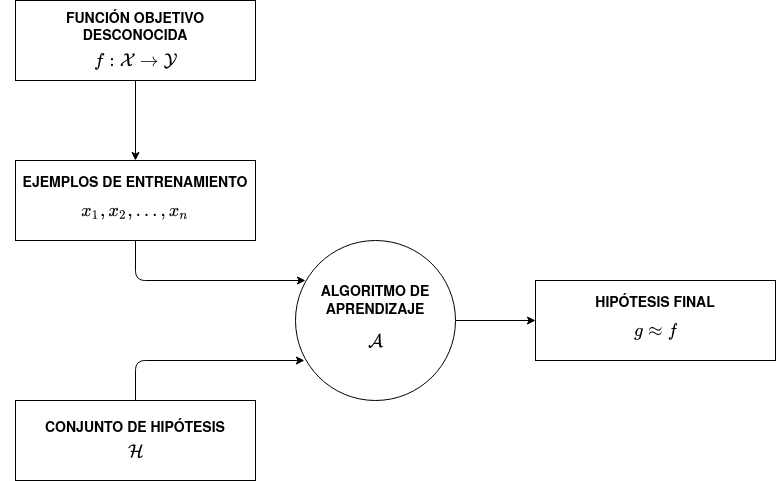
\includegraphics[width=1\textwidth]{problema-aprendizaje}
  \caption{Componentes de un problema de aprendizaje automático}
  \label{fig:problema-aprendizaje}
\end{figure}

Las tareas y experiencias pueden ser muy diversas, lo que nos permite diferenciar varios tipos de algoritmos. Según el tipo de experiencia, en general podemos diferenciar entre aprendizaje supervisado cuando al algoritmo se le proporciona un conjunto de ejemplos para los cuales la tarea está ya resuelta o no supervisado cuando el algoritmo cuenta solo con ejemplos que no están resueltos. Cuando se trabaja con ejemplos resueltos y sin resolver se trata de aprendizaje semi-supervisado, y cuando no se proporciona una respuesta a cada ejemplo pero sí se asigna una puntuación a cada posible respuesta se trata de aprendizaje por refuerzo. Algunas de las tareas a las que pueden aplicarse son:

\begin{itemize}
  \item Clasificación: el programa debe deducir a qué clase pertenece cada instancia de los datos.
  \item Regresión: el programa debe asignar un valor real a cada instancia.
  \item Síntesis y muestreo: el programa debe generar nuevos ejemplos parecidos a los usados para su entrenamiento.
\end{itemize}

Una primera aproximación a la solución de problemas de aprendizaje son los modelos lineales, como el de regresión lineal o regresión logística, modelos cuyo conjunto de hipótesis es de funciones lineales sobre el conjunto de entrada. Su principal desventaja es su limitación a la hora de aproximar funciones no lineales, ya que no son capaces de expresar las posibles interacciones entre variables.

Existen también modelos no lineales, entre los que se encuentran los modelos basados en árboles de decisióno modelos basando en distancias entre ejemplos como los $k$ vecinos más cercanos. Estos modelos sí permiten modelar relaciones no lineales entre los datos.

El aprendizaje profundo o \textit{deep learning} es una rama del aprendizaje automático basada en el uso de redes neuronales. Surge en parte como respuesta al problema de los modelos lineales, ya que permite la aproximación de funciones no lineales mediante el aprendizaje de sucesivas transformaciones no lineales de los datos de entrada. En este apartado se introducen estos modelos y su entrenamiento.

\section{Redes neuronales prealimentadas}

Las redes prealimentadas profundas, redes neuronales profundas o perceptrones multicapa, \textit{deep feedforward networks}, \textit{feedforward neural networks} o \textit{multilayer perceptron} (MLP) en inglés, son el modelo canónico del aprendizaje profundo~\cite{abu2012learning}. Su objetivo es aproximar la función $f^*$ mediante una aplicación $f(\textbf{x};\theta)$ y aprendiendo el valor de los parámetros $\theta$ que permita un mejor resultado.

Se llaman redes ya que suelen representarse componiendo varias funciones diferentes. El modelo puede asociarse con un grafo dirigido acíclico que describe cómo se componen las funciones. Un ejemplo de esta estructura es, teniendo tres funciones vectoriales $f_1$, $f_2$ y $f_3$, componerlas de la forma $f(\textbf{x}) = f_3(f_2(f_1(\textbf{x})))$. En este caso la función $f_i$ se llama capa i-ésima de la red. La longitud de la cadena es la profundidad de la red, de donde surge la nomeclatura redes profundas. La última capa de la red se llama capa de salida.

\begin{figure}[htpb]
  \centering
  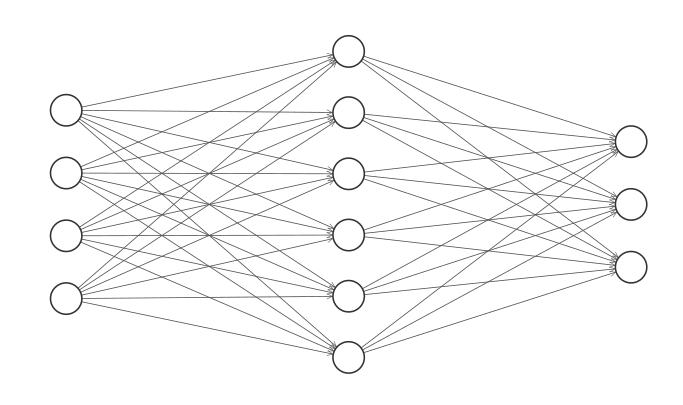
\includegraphics[width=1\textwidth]{nn}
  \caption{Ejemplo de red neuronal prealimentada de profundidad 3}
  \label{fig:nn}
\end{figure}


Durante el entrenamiento se intenta conseguir que $f(\textbf{x})$ se aproxime a $f^*(\textbf{x})$. Los datos del conjunto de entrenamiento ofrecen ejemplos, aproximados y ruidosos, de la función $f^*$ evaluada en diferentes $\textbf{x} \in \mathcal{X}$. Cada ejemplo \textbf{x} está normalmente acompañado de una salida deseada $\textbf{y} \approx f^*(\textbf{x})$. Así, los ejemplos especifican qué resultado debe ofrecer la capa de salida para cada uno de ellos. El comportamiento del resto de capas no está especificado, y es el algoritmo de aprendizaje el que debe configurarlo para obtener la mejor aproximación de $f^*$.

Que el grafo sea acíclico implica que no existe retroalimentación con la salida de ninguna de las unidades de la red. Cuando el modelo se extiende para permitir la retroalimentación se trata de una red neuronal recurrente, que veremos posteriormente.

El componente básico de cada una de las capas, al que llamamos unidad, consiste en una función de $\mathbb{R}^n$ en $\mathbb{R}$, donde $n$ es el tamaño de la capa anterior. Cada unidad recibe la salida de las unidades de la capa anterior y calcula un valor que devuelve, su valor de activación. Este comportamiento se inspira en las neuronas biológicas ~\cite{izenman2008modern}, por eso este tipo de modelos recibe el nombre de red neuronal.

Puesto que el objetivo es aproximar funciones no lineales, no basta con que las transformaciones que aplican estas unidades sean transformaciones lineales de los datos de entrada. De ser así, podríamos resumir el comportamiento de la red al completo en una única transformación lineal. Se busca por tanto el aprendizaje de una transformación no lineal $\phi$ de entre una clase de funciones parametrizadas. Se define así un modelo del tipo $$y = f(\textbf{x};\theta,\textbf{w}) = \phi(\textbf{x};\theta)^T\textbf{w}$$ donde $\theta$ es un vector de parámetros que permite seleccionar $\phi$ de entre la familia que elegimos y $w$ se utiliza para aplicar la transformación de los datos obtenida en la salida deseada. La clase de funciones de entre los que el modelo busca la aproximación, el conjunto de hipótesis, se determina al seleccionar la estructura de la red y los tipos de unidades ocultas y de salida.


\subsection{Función de coste}

La mayoría de diseños de redes neuronales se realizan definiendo la distribución $P(y|x;\theta)$ y aplicando el principio de máxima verosimilitud. Si $\textbf{X} = \{\textbf{x}_1,...,\textbf{x}_n\}$ representa los ejemplos, $\textbf{Y} = \{\textbf{y}_1,...,\textbf{y}_n\}$ sus soluciones, el estimador de máxima verosimilitud vendrá dado por $$\theta_{ML} = \arg \max_{\theta} P(\textbf{Y}|\textbf{X}; \theta).$$
Asumiendo que los ejemplos son independientes e idénticamente distribuidos
$$\theta_{ML} = \arg \max_{\theta} \prod_{i=1}^n P(\textbf{y}_i|\textbf{x}_i; \theta).$$

Puesto que el logaritmo es una función estrictamente creciente, tomar el logaritmo nos da un problema de optimización equivalente, por lo que $$\theta_{ML} = \arg \max_{\theta} \sum_{i=1}^n \log P(\textbf{y}_i|\textbf{x}_i; \theta).$$

Escalar la función tampoco cambia cuál es el máximo, por lo que podemos dividir entre $n$ para obtener una expresión respecto de la esperanza de la distribución empírica $\hat{P}_{\text{data}}$ de los datos de entrenamiento

$$\theta_{ML} = \frac{1}{n} \arg \max_{\theta} \sum_{i=1}^n \log P(\textbf{y}_i|\textbf{x}_i; \theta) = \mathbb{E}_{\textbf{x}, \textbf{y} \sim \hat{P}_{\text{data}}}\log P(\textbf{y}|\textbf{x}).$$

Teniendo esto, podemos definir la función de coste como
$$J(\theta) = -\mathbb{E}_{\textbf{x}, \textbf{y} \sim \hat{P}_{\text{data}}}\log P(\textbf{y}|\textbf{x}).$$

La expresión concreta de la función de coste cambia con el modelo, dependiendo de la distribución $P$. Normalmente también se añade un término de regularización. Con este, la función de coste es de la forma
$$J(\theta) = -\mathbb{E}_{\textbf{x}, \textbf{y} \sim \hat{P}_{\text{data}}}\log P(\textbf{y}|\textbf{x}) + \lambda \Omega (\theta).$$

\subsection{Unidades de salida}

Siguiendo el método previo, la elección de la representación de la salida de una red prealimentada determina la expresión de su función de coste. En esta sección estudiamos qué tipo de unidades suelen utilizarse como salida de la red. Para ello supondremos que las unidades ocultas nos proporcionan un vector de características $\textbf{h} = f(\textbf{x};\theta)$. La capa de salida transforma estas características para completar la tarea que la red debe cumplir.

\subsubsection{Unidades lineales}

Dadas las características $\textbf{h}$, una capa con unidades lineales produce un vector $\textbf{y} = \textbf{W}^T \textbf{h} + \textbf{b}$, sin transformaciones no lineales. Suelen usarse para producir la media de una distribución condicional normal $$p(\textbf{y}|\textbf{x}) = \mathcal{N}(\textbf{y}^*; \textbf{y},I).$$ En este caso obtener la máxima verosimilitud equivale a minimizar el error cuadrático medio.

\subsubsection{Unidades con activación sigmoidal}

Muchas tareas requieren predecir una variable binaria $y$. Un ejemplo de ello son los problemas de clasificación con dos clases. En este caso la aproximación del método de máxima verosimilitud es definir una distribución de Bernouilli sobre $y$ condicionada a $\textbf{x}$. La red neuronal tendrá entonces que predecir $P(y=1| \textbf{x})$. El número generado por la red, por tanto, estará en el intervalo $[0,1]$.

Para un correcto entrenamiento mediante técnicas basadas en gradiente es necesario que no genere un gradiente nulo o muy cercano a $0$ cuando el modelo no se acerque a la solución. Para ello se aplica una función de activación sigmoidal a la salida, como la función logística $$y = \sigma (\textbf{w}^T\textbf{h} + b) = \frac{1}{1 + e^{-(\textbf{w}^T\textbf{h} + b)}}.$$

Definamos entonces una distribución de probabilidad sobre $y$ usando el valor de $z = \textbf{w}^T\textbf{h} + b$. La elección de la función de activación sigmoidal puede justificarse construyendo una distribución de probabilidad no normalizada $\hat{P}$(y), cuya suma no es 1, que supondremos $\log$-lineal en $z$ e $y$. Entonces podemos exponenciar para obtener una distribución de probabilidad válida y normalizando obtendremos una distibución de Bernouilli controlada por una transformación sigmoidal de $z$:

$$\log \hat{P}(y) = yz$$ $$\hat{P}(y) = e^{yz}$$ \\ $$P(y) = \frac{e^{yz}}{e^{0z}+e^{1z}} = \frac{e^{yz}}{1+e^z} = \sigma((2y-1)z). $$

De esta manera la función de coste es $$J(\theta) = -\log P(y|\textbf{x}) = - \log \sigma((2y-1)z).$$ Esta función solo se satura cuando $y = 1$ y $z$ es muy positivo o cuando $y = 0$ y $z$ es muy negativo, es decir, cuando el modelo alcanza la respuesta. Esta función está bien definida ya que cualquier función sigmoidal toma valores en $(0,1)$, y por tanto el logaritmo es finito.

\subsubsection{Unidades softmax}

La función de activación softmax puede utilizarse para representar una distribución de probabilidad sobre una variable discreta con $n$ valores posibles. Este es el caso de los problemas de clasificación con más de dos clases. Puede interpretarse por tanto como una generalización para las funciones de activación sigmoidal.

En este caso se necesita generar un vector $\textbf{y}$, con $y_i = P(y = i| \textbf{x})$. Cada elemento de $\textbf{y}$ debe estar en $[0,1]$, y la suma de todos ellos debe ser 1 para representar una distribución de probabilidad válida.

Siguiendo el razonamiento anterior, una capa lineal predice probabilidades logarítmicas no normalizadas, $$\textbf{z} = \textbf{W}^T \textbf{h} + b$$ donde $z_i = \log \hat{P}(y = i | \textbf{x})$. La función softmax, definida componente a componente como $$\text{softmax}(\textbf{z})_i = \frac{e^{z_i}}{\sum_j e^{z_j}}, $$  exponencia y normaliza $\textbf{z}$ para obtener la $\textbf{y}$ deseada. Igual que en el caso anterior, la función de coste puede obtenerse aplicando el principio de máxima verosimilitud.

\subsection{Unidades ocultas}\label{unidades-ocultas}

Cualquiera de los tipos de unidad anterior puede utilizarse en una capa oculta, pero existen más diseños. En este apartado se describen algunos de los tipos más comunes. Por lo general, las capas ocultas aceptan un vector de entrada $\textbf{x}$ sobre el que realizan una transformación afín $\textbf{z} = \textbf{W}^T\textbf{x} + \textbf{b}$, donde la matriz $\textbf{W}$ se llama matriz de pesos y el vector $\textbf{b}$ vector de sesgo, y después aplican una transformación no lineal $g(\textbf{z})$, llamada función de activación. La elección de esta transformación es la que marca el tipo de unidad que se selecciona.

Algunas de las unidades ocultas aquí expuestas no son diferenciables en todos los puntos. Podría parecer que esto las invalida para el aprendizaje mediante métodos de gradiente. En la práctica el descenso del gradiente funciona bien con estas funciones de activación ya que no se suele llegar a un mínimo de la función de coste, sino reducir su valor. Por ello no se obtendrá un valor en el que el gradiente sea nulo, y es aceptable que el mínimo de la función de coste corresponda a valores en los que el gradiente no está definido. Por lo tanto, en la práctica, pueden no tenerse en cuenta los puntos en los que las funciones aquí descritas no son diferenciables.

\subsubsection{Unidades lineales rectificadas}\label{unidades-relu}

Las unidades lineales rectificadas (\textit{ReLU}) utilizan la función de activación $g(\textbf{z})_i = \max\{0,z_i\}$.

\begin{figure}[htpb]
  \centering
  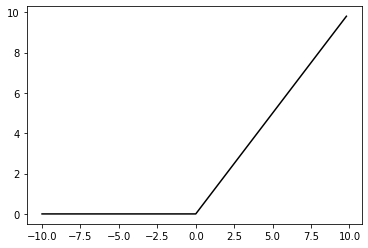
\includegraphics[width=0.6\textwidth]{relu}
  \caption{Gráfica de la función \textit{ReLU}}
  \label{fig:relu}
\end{figure}

Estas unidades son fáciles de optimizar por su parecido a las unidades lineales. La única diferencia con estas es que las rectificadas se anulan en la mitad de su dominio. Existen múltiples generalizaciones de este tipo de unidades:

\begin{itemize}
\item Rectificación mediante valor absoluto: $g(\textbf{z})_i = \lvert z_i \rvert$.
\item Leaky \textit{ReLU}: $g(\textbf{z})_i = \max \{0,z_i\} + \alpha \min \{0,z_i\}$ con un $\alpha$ fijo, normalmente $0,01$.
\item \textit{ReLU} paramétríca: $g(\textbf{z})_i = \max\{0,z_i\} + \alpha_i \min \{0,z_i\}$ con $\alpha_i$ un parámetro optimizable.
\end{itemize}

\begin{figure}[htpb]
  \centering
  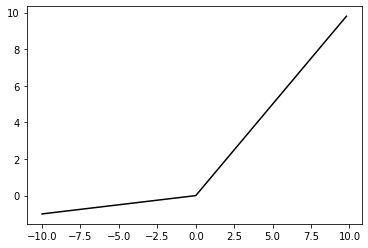
\includegraphics[width=0.6\textwidth]{leakyrelu}
  \caption{Gráfica de la función \textit{leaky ReLU} con $\alpha = 0,1$}
  \label{fig:leakyrelu}
\end{figure}


Otra generalización importante son las unidades maxout, que agrupa los elementos de $z$ en subconjuntos de $k$ elementos. Cada una de las unidades de una capa de este tipo devuelve el máximo de uno de estos subconjuntos. Así,

$$ g(\textbf{z})_i = \max_{j \in \mathbb{G}(i)} z_j$$

donde $\mathbb{G}(i) = \{(i-1)k +1,...,ik\}$ es el conjunto de índices para el subconjunto $i$-ésimo. Una capa de estas unidades puede aprender una función convexa lineal a trozos de hasta $k$ trozos. Podemos considerar que más que la relación entre las unidades, estas capas aprenden la función de activación misma. Con un $k$ suficientemente grande, estas unidades pueden aprende a aproximar cualquier función convexa con precisión arbitraria~\cite{goodfellow2016}.

\subsubsection{Unidades con activación sigmoidal}

Otras dos unidades comunes utilizan funciones sigmoidales, la función logística

$$g(\textbf{z})_i = \sigma(z_i) = \frac{1}{1+e^{-z_i}}$$

\begin{figure}[htpb]
  \centering
  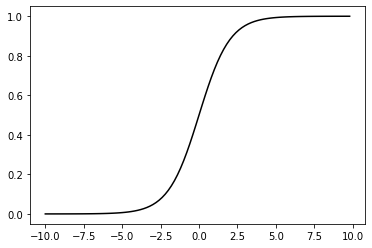
\includegraphics[width=0.6\textwidth]{logistica}
  \caption{Gráfica de la función logística}
  \label{fig:logistica}
\end{figure}

y la función tangente hiperbólica

$$g(\textbf{z})_i = \tanh(z_i) = \frac{e^{z_i} - e^{-z_i}}{e^{z_i}+e^{-z_i}}.$$

\begin{figure}[htpb]
  \centering
  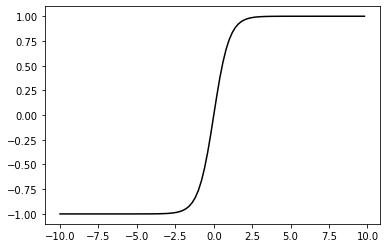
\includegraphics[width=0.6\textwidth]{tanh}
  \caption{Gráfica de la función tangente hiperbólica}
  \label{fig:tanh}
\end{figure}

Estas dos funciones están muy relacionadas, ya que $\tanh (z) = 2 \sigma (2z) - 1$. Las funciones sigmoidales se saturan en gran parte de su dominio, lo que puede dificultar el aprendizaje. Es por ello que su uso ha disminuido desde la introducción de las \textit{ReLU}.

\subsection{Propagación hacia adelante}

Una vez configurada la red, esta recibe una entrada que se propaga a través de cada una de las capas, que le aplican las transformaciones correspondientes hasta la salida. Este proceso se llama propagación hacia adelante, y se describe en el algoritmo \ref{feedforward-propagation}.


\begin{algorithm}
\label{feedforward-propagation}
 \caption{Propagación hacia adelante en una red neuronal profunda con función de activación $g$ para una entrada \textbf{x}.}
     \SetAlgoLined
     \KwIn{$\ell$ profundidad de la red}
     \KwIn{$\textbf{W}_i$ matriz de pesos de la capa $i$-ésima, $i = 1,...,\ell$}
     \KwIn{$\textbf{b}_i$ vector de sesgos de la capa $i$-ésima, $i = 1,...,\ell$}
     \KwIn{$\textbf{x}$ entrada de la red}
     $\textbf{h}_0 \leftarrow \textbf{x}$\;
     \For{$i = 1,...,\ell$}{
      $\textbf{z}_i \leftarrow (\textbf{W}_{i})^T\textbf{x}_{i-1} + \textbf{b}_i$\;
      $\textbf{h}_i \leftarrow g_i(\textbf{z}_i)$\;
     }
     $\textbf{y} \leftarrow \textbf{h}_{\ell}$\;
\end{algorithm}


\section{Entrenamiento de redes neuronales prealimentadas}

\subsection{Optimización}\label{optimizacion}

Una vez conocida la función de coste $J(\theta)$ el siguiente paso es buscar unos parámetros $\theta$ que la minimicen. Para resolver este problema de optimización, al menos de forma aproximada, se aplica la técnica del descenso del gradiente. Este método fue inicialmente propuesto por Cauchy~\cite{cauchy1847methode} en 1847 y su convergencia fue estudiada por primera vez por Curry~\cite{curry1944method} en 1944.

\subsubsection{Descenso del gradiente}

Sea $f$ un campo escalar de $S \subset \mathbb{R}^n$ en $\mathbb{R}$, continuo en $S$ y derivable con derivada continua en el interior de $S$. La dirección en la que la función desciende más rápidamente vendrá dada por la del vector $$- \varepsilon \nabla f(x_1,...x_n) = \left( -\varepsilon \frac{\partial f}{\partial x_1}(x_1,...,x_n), ..., - \varepsilon \frac{\partial f}{\partial x_n}(x_1,...,x_n) \right),$$ donde $\varepsilon > 0$ es un factor de proporcionalidad al que suele llamarse tasa de aprendizaje. El método consiste en, desde un punto inicial $\textbf{x}_0$ e iterativamente, calcular el opuesto del gradiente y avanzar en esa dirección una distancia determinada por $\varepsilon$. Así, en la iteración $i$-ésima, $\textbf{x}^{(i)} = \textbf{x}^{(i-1)} - \varepsilon \nabla f(\textbf{x}^{(i-1)})$.  El algoritmo termina cuando el valor de $\nabla f(x_1,...,x_n)$ es cercano a cero, con una tolerancia dada.

La convergencia del proceso al mínimo está probada cuando el mínimo de la función sobre la que se aplica es único. Este no es el caso de las funciones a las que se aplica en el contexto del aprendizaje profundo. Las funciones de coste que se intentan optimizar pueden tener muchos mínimos locales o puntos de silla en los que el algoritmo puede terminar sin obtener una buena solución. Otro inconveniente importante es el coste computacional que supone la aplicación del algoritmo a muestras grandes de datos, como suele hacerse en el aprendizaje automático para obtener modelos suficientemente generales. Es por ello que en la práctica se utilizan versiones del procedimiento que responden a estas cuestiones.

\subsubsection{Descenso del gradiente estocástico (SGD)}

La aplicación del descenso del gradiente a un problema de aprendizaje automático se realiza calculando la media aritmética de los gradientes de la función de pérdida para cada uno de los datos del conjunto de entrenamiento. Esto implica evaluar la función de coste para cada ejemplo del conjunto de entrenamiento antes de actualizar el gradiente, lo que puede ser computacionalmente inasumible. Es por ello que en la actualidad la técnica más usada es una aproximación en la que se utiliza un solo ejemplo para cada actualización. Este es, en la actualidad, el algoritmo más utilizado. Se describe detalladamente en \ref{sgd}.

\begin{algorithm}
\label{sgd}
 \caption{Algoritmo de descenso del gradiente estocástico.}
     \SetAlgoLined
     \KwIn{$\theta$ vector inicial de parámetros}
     \KwIn{$\varepsilon$ tasa de aprendizaje}
     \KwIn{$\textbf{x}_1,...,\textbf{x}_n$ ejemplos de entrenamiento}
     \KwIn{$\textbf{y}_1,...,\textbf{y}_n$ objetivo de cada ejemplo}
     \While{no se alcanza un mínimo aproximado}{
      Mezclar aleatoriamente los ejemplos del conjunto de entrenamiento\;
      \For{$i = 1,...,n$}{
        $\theta \leftarrow \theta - \varepsilon \nabla L( f(\textbf{x}_i; \theta),\textbf{y}_i)$\;
      }
     }
\end{algorithm}

\subsubsection{Variantes de SGD}

Mediante la aplicación de SGD se mitiga el problema del coste computacional del descenso del gradiente, pero la posibilidad de terminar en un mínimo local no óptimo o en un punto de silla sigue existiendo. Además, la aproximación que realiza SGD del gradiente puede no ser suficientemente buena. Existen diferentes alternativas que afrontan estos problemas.

\begin{itemize}
\item Gradiente descendente estocástico con minilotes: para realizar una aproximación más fiel del gradiente de la función toma minilotes de elementos del conjunto de entrenamiento en lugar de un solo elemento. Se describe detalladamente en \ref{sgd-minilotes}.
\item Método del momento~\cite{sutskever2013training}: en cada paso se recuerda la anterior actualización y la siguiente se calcula como una combinación lineal entre esta y el gradiente. De esta manera la variación de la dirección de una iteración a otra disminuye, evitando el comportamiento de zigzagueo. Se describe detalladamente en \ref{momentum}.
\item AdaGrad~\cite{duchi2011adaptive}: se basa en adaptar la tasa de aprendizaje para cada parámetro de forma inversamente proporcional a la raíz cuadrada de la suma de los valores anteriores. Así se decrementa más rápidamente la tasa de aprendizaje para los parámetros con mayor derivada parcial y se progresa más rápidamente en las zonas de menor pendiente. Se describe detalladamente en \ref{adagrad}.
\item RMSProp~\cite{tieleman2012lecture}: similar a adagrad, modifica la tasa de aprendizaje para cada parámetro. En este caso se cambia la acumulación del gradiente por una media con pesos exponenciales para mejorar su comportamiento en funciones no convexas. Se describe detalladamente en \ref{rmsprop}.
\item Adam~\cite{kingma2014adam}: es otro algoritmo con tasa de aprendizaje adaptativa. Es una combinación entre RMSProp y método del momento, ya que añade un momento adaptativo. Se describe detalladamente en \ref{adam}.
\end{itemize}

\begin{algorithm}
\label{sgd-minilotes}
 \caption{Algoritmo de descenso del gradiente estocástico con minilotes.}
     \SetAlgoLined
     \KwIn{$\theta$ vector inicial de parámetros}
     \KwIn{$m$ tamaño de minilote}
     \KwIn{$\varepsilon$ tasa de aprendizaje}
     \KwIn{$\textbf{x}_1,...,\textbf{x}_n$ ejemplos de entrenamiento}
     \KwIn{$\textbf{y}_1,...,\textbf{y}_n$ objetivo de cada ejemplo}
     \While{no se alcanza un mínimo aproximado}{
      Seleccionar un minilote de $m$ ejemplos del conjunto de entrenamiento $\{\textbf{x}_1,...,\textbf{x}_m\}$ y sus correspondientes objetivos $\textbf{y}_i$\;
        $\theta \leftarrow \theta - \frac{\varepsilon}{m} \nabla \sum_i L( f(\textbf{x}_i; \theta),\textbf{y}_i)$\;

     }
\end{algorithm}

\begin{algorithm}
\label{momentum}
 \caption{SGD con método del momento.}
     \SetAlgoLined
     \KwIn{$\theta$ vector inicial de parámetros}
     \KwIn{$\varepsilon$ tasa de aprendizaje}
     \KwIn{$\alpha$ valor del momento}
     \KwIn{$v$ velocidad inicial}
     \KwIn{$\textbf{x}_1,...,\textbf{x}_n$ ejemplos de entrenamiento}
     \KwIn{$\textbf{y}_1,...,\textbf{y}_n$ objetivo de cada ejemplo}
     \While{no se alcanza un mínimo aproximado}{
     Seleccionar un minilote de $m$ ejemplos del conjunto de entrenamiento $\{\textbf{x}_1,...,\textbf{x}_m\}$ y sus correspondientes objetivos $\textbf{y}_i$\;
     $v \leftarrow \alpha v - \frac{\varepsilon}{m} \nabla \sum_i L( f(\textbf{x}_i; \theta),\textbf{y}_i)$\;
     $\theta \leftarrow \theta + v$\;

     }
\end{algorithm}

\begin{algorithm}
\label{adagrad}
 \caption{Adagrad. $\odot$ representa el producto componente a componente, $\sqrt{\cdot}$ la raíz cuadrada componente a componente y la división $\frac{\varepsilon}{\delta + \sqrt{r}}$ se realiza componente a componente.}
     \SetAlgoLined
     \KwIn{$\theta$ vector inicial de parámetros}
     \KwIn{$\delta$ constante pequeña, normalmente $10^{-6}$}
     \KwIn{$\varepsilon$ tasa de aprendizaje inicial}
     \KwIn{$\textbf{x}_1,...,\textbf{x}_n$ ejemplos de entrenamiento}
     \KwIn{$\textbf{y}_1,...,\textbf{y}_n$ objetivo de cada ejemplo}
     $r \leftarrow 0$\;
     \While{no se alcanza un mínimo aproximado}{
      Seleccionar un minilote de $m$ ejemplos del conjunto de entrenamiento $\{\textbf{x}_1,...,\textbf{x}_m\}$ y sus correspondientes objetivos $\textbf{y}_i$\;
        $g \leftarrow \frac{1}{m} \nabla \sum_i L( f(\textbf{x}_i; \theta),\textbf{y}_i)$\;
        $r \leftarrow r + g \odot g$\;
        $\theta \leftarrow \theta - \frac{\varepsilon}{\delta + \sqrt{r}} \odot g$\;
     }
\end{algorithm}

\begin{algorithm}
\label{rmsprop}
 \caption{RMSProp. $\odot$ representa el producto componente a componente, $\sqrt{\cdot}$ la raíz cuadrada componente a componente y la división $\frac{\varepsilon}{\delta + \sqrt{r}}$ se realiza componente a componente.}
     \SetAlgoLined
     \KwIn{$\theta$ vector inicial de parámetros}
     \KwIn{$\rho$ ratio de decaimiento}
     \KwIn{$\delta$ constante pequeña, normalmente $10^{-6}$}
     \KwIn{$\varepsilon$ tasa de aprendizaje inicial}
     \KwIn{$\textbf{x}_1,...,\textbf{x}_n$ ejemplos de entrenamiento}
     \KwIn{$\textbf{y}_1,...,\textbf{y}_n$ objetivo de cada ejemplo}
     $r \leftarrow 0$\;
     \While{no se alcanza un mínimo aproximado}{
      Seleccionar un minilote de $m$ ejemplos del conjunto de entrenamiento $\{\textbf{x}_1,...,\textbf{x}_m\}$ y sus correspondientes objetivos $\textbf{y}_i$\;
        $g \leftarrow \frac{1}{m} \nabla \sum_i L( f(\textbf{x}_i; \theta),\textbf{y}_i)$\;
        $r \leftarrow \rho r + (1 - \rho) g \odot g$\;
        $\theta \leftarrow \theta - \frac{\varepsilon}{\delta + \sqrt{r}} \odot g$\;
     }
\end{algorithm}

\begin{algorithm}
\label{adam}
 \caption{Adam. $\odot$ representa el producto componente a componente, $\sqrt{\cdot}$ la raíz cuadrada componente a componente y la división $\frac{\varepsilon}{\delta + \sqrt{r}}$ se realiza componente a componente.}
     \SetAlgoLined
     \KwIn{$\theta$ vector inicial de parámetros}
     \KwIn{$\rho_1, \rho_2 \in [0,1)$ ratios de decaimeiento exponencial, sugeridos por defecto $0,9$ y $0,99$}
     \KwIn{$\delta$ constante pequeña, normalmente $10^{-6}$}
     \KwIn{$\varepsilon$ tasa de aprendizaje inicial}
     \KwIn{$\textbf{x}_1,...,\textbf{x}_n$ ejemplos de entrenamiento}
     \KwIn{$\textbf{y}_1,...,\textbf{y}_n$ objetivo de cada ejemplo}
     $r \leftarrow 0$\;
     $s \leftarrow 0$\;
     $t \leftarrow 0$\;
     \While{no se alcanza un mínimo aproximado}{
      Seleccionar un minilote de $m$ ejemplos del conjunto de entrenamiento $\{\textbf{x}_1,...,\textbf{x}_m\}$ y sus correspondientes objetivos $\textbf{y}_i$\;
        $g \leftarrow \frac{1}{m} \nabla \sum_i L( f(\textbf{x}_i; \theta),\textbf{y}_i)$\;
        $t \leftarrow t+1$\;
        $r \leftarrow \rho_1 r + (1 - \rho_1) g$\;
        $r \leftarrow \rho_2 r + (1 - \rho_2) g \odot g$\;
        $\hat{s} \leftarrow \frac{s}{1 - \rho_1^t}$\;
        $\hat{r} \leftarrow \frac{s}{1 - \rho_2^t}$\;
        $\theta \leftarrow \theta - \frac{\hat{s}}{\sqrt{\hat{r}}+\delta} \odot g$\;
     }
\end{algorithm}

\subsection{Propagación hacia atrás}\label{back-propagation}

El cálculo del gradiente de la función de coste es básico para el entrenamiento de redes neuronales. Obtener su expresión analítica es sencillo, pero evaluar numéricamente esa expresión puede ser muy costoso computacionalmente. El algoritmo de propagación hacia atrás (\textit{back propagation}) permite realizar este cálculo de manera eficiente, utilizando la regla de la cadena para evitar repetir el cálculo de derivadas parciales que aparecen varias veces en el proceso.

Tras aplicar propagación hacia adelante se aplica el algoritmo descrito en \ref{backprop}, que obtiene los gradientes de la función de activación de cada capa, empezando por la capa de salida y yendo hacia atrás hasta la primera capa oculta. De estos gradientes, que pueden ser interpretados como la indicación de cómo la salida de cada capa debería cambiar para reducir el error, se puede obtener el gradiente respecto de los parámetros de cada capa. Obtenido el gradiente respecto de los pesos y los sesgos, puede utilizarse para aplicar alguno de los métodos de optimización basados en gradiente.

\begin{algorithm}
\label{backprop}
 \caption{Propagación hacia atrás con entrada $\textbf{x}$, salida $\textbf{y}$, objetivo $\textbf{y}^*$ y profundidad $\ell$. $L$ representa la función de coste sin regularización, y $J$ la función de coste completa. $\odot$ denota el producto componente a componente.}
     \SetAlgoLined
     $\textbf{d} \leftarrow \nabla_\textbf{y} J(\textbf{y},\textbf{y}^*;\theta) = \nabla_\textbf{y} L(\textbf{y},\textbf{y}^*)$\;
     \For{$k = \ell,...,1$}{
      $\textbf{d} \leftarrow \nabla_{\textbf{z}_k} J = \textbf{d} \odot g'(\textbf{z}_k)$\;
      $\nabla_{\textbf{b}_k} J = \textbf{d} + \lambda \nabla_{\textbf{b}_k} \Omega(\theta)$\;
      $\nabla_{\textbf{W}_k} J = \textbf{d}(h_{k-1})^T + \lambda \nabla_{\textbf{W}_k} \Omega(\theta)$\;
      $\textbf{d} \leftarrow \nabla_{h_{k-1}}J = (\textbf{W}_k)^T \textbf{d}$\;
     }

\end{algorithm}

\endinput
%------------------------------------------------------------------------------------
% FIN DEL CAPÍTULO.
%------------------------------------------------------------------------------------

% !TeX root = ../libro.tex
% !TeX encoding = utf8

\chapter{Tratamiento de secuencias}

Hasta ahora se han descrito redes neuronales que tratan los datos de manera aislada. Cada instancia es procesada independientemente y se asigna una salida solo en función de la entrada facilitada. No existe ningún tipo de realimentación en la red. Esta estructura es adecuada para, por ejemplo, problemas de clasificación en los cuales los datos son independientes entre sí y la clasificación de un ejemplo no debería afectar a la del resto. Sin embargo pueden plantearse muchos problemas de aprendizaje en los que no exista tal independencia. El contexto de un ejemplo puede ser relevante para su resolución.

Un caso de este tipo de problemas es el tratamiento de secuencias, conjuntos de datos ordenados en los cuales cada instancia tiene cierta relación con sus antecesores y predecesores. Algunos tipos de datos que podemos interpretar como secuencias son textos, vídeos, grabaciones de voz, cadenas de ADN o música. En las tareas que impliquen su manejo será relevante tener en cuenta la relación de cada elemento con los previos y posteriores. Algunos ejemplos de problemas en los que se usan son:

\begin{itemize}
  \item Generación de texto~\cite{lu2018neural}: consiste en producir texto en lenguaje natural. Puede aplicarse a multitud de fines, entre los que se incluyen completar textos automáticamente, generación de poemas o descripción textual de vídeo o imágenes.
  \item Traducción automática~\cite{singh2017machine}: conversión automática de un lenguaje natural a otro lenguaje natural diferente.
  \item Análisis de secuencias de ADN~\cite{liu2019detection}: dada una secuencia de ADN, detección de determinadas estructuras o modificaciones en el mismo.
  \item Reconocimiento de voz~\cite{graves2013speech}: transcripción del lenguaje hablado captado como audio a texto.
  \item Análisis de sentimientos~\cite{valdivia2017sentiment}: identificación y clasificación de opiniones expresadas en forma de texto para determinar si la actitud de su autor hacia un tema concreto es positiva, negativa o neutral.
  \item Generación de música: creación automática de música. Algunas de las aproximaciones existentes son completar una obra parcialmente compuesta con acompañamientos y contrapunto ~\cite{huang2017counterpoint} o generar música con un estilo determinado ~\cite{carr2018generating}.
\end{itemize}

Además de la dependencia entre elementos es también destacable que por su naturaleza secuencial, los datos con los que trabaja este tipo de problemas pueden ser más extensos de lo que sería práctico computar mediante una red prealimentada profunda. Además pueden tener extensiones diferentes, lo que también resulta problemático. Es por ello que su tratamiento mediante las técnicas vistas hasta ahora resulta muy difícil y se hace necesaria la utilización de modelos especializados.

La principal idea a la hora de enfrentar tareas de esta índole es añadir retroalimentación a la red. De esta manera puede conservarse información a través de las diferentes resoluciones de ejemplos. Cuando se incluye esta característica estamos ante modelos llamados redes neuronales recurrentes (RNN), \textit{recurrent neural networks} en inglés. En este capítulo se repasan las arquitecturas más importantes de este tipo y cómo se afronta el problema de la dependencia entre instancias y la conservación de información entre las sucesivas resoluciones.

\section{Redes neuronales recurrentes}

En este apartado consideramos una secuencia como un conjunto finito de ejemplos $\{\textbf{x}^{(1)},\textbf{x}^{(2)},...,\textbf{x}^{(T)}\}$. Diremos que la secuencia tiene longitud $T$. La idea de introducir retroalimentación en la red es equivalente a introducir un nuevo parámetro a la función que representa la red, al cual llamaremos estado o estado oculto. En cada posición o instante $t$ el estado $\textbf{h}^{(t)}$ dependerá del estado anterior $\textbf{h}^{(t-1)}$ y de la entrada actual $\textbf{x}^{(t)}$. De igual manera, la salida del instante $t$, $\textbf{y}^{(t)}$ ya no solo dependerá de la entrada $\textbf{x}^{(t)}$ y los parámetros $\theta$, sino también del estado anterior $\textbf{h}^{(t-1)}$.

\begin{figure}[htpb]
  \centering
  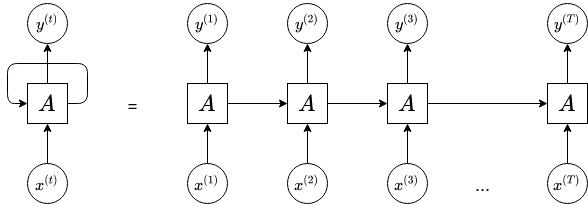
\includegraphics[width=1\textwidth]{recurrent}
  \caption{Desenrollado de una red neuronal recurrente}
  \label{fig:recurrent}
\end{figure}

Para realizar la propagación hacia adelante en una red recurrente como la de la figura (insertar cita a figura anterior) basta con aplicar las siguientes ecuaciones en cada paso $t$, desde $t=1$ hasta $t=T$:
$$\textbf{h}^{(t)} = g_1(\textbf{b} + \textbf{W}\textbf{h}^{(t-1)} + \textbf{U}\textbf{x}^{(t)}), $$
$$\textbf{y}^{(t)} = g_2(\textbf{c} + \textbf{V}\textbf{h}^{(t)}) $$

donde los parámetros son los vectores de de sesgos $\textbf{b}$ y $\textbf{c}$ junto con las matrices de pesos $\textbf{U}$, $\textbf{V}$ y $\textbf{W}$, que conectan la entrada con el estado oculto, el estado oculto con la salida y el estado oculto actual con el siguiente, respectivamente. Las funciones $g_1$ y $g_2$ son funciones de activación que pueden ser diferentes, siendo la primera normalmente una función ReLU o tangente hiperbólica y encargada de generar el siguiente estado y la segunda la encargada de la salida de la red, lo cuál condicionará su forma. Es importante tener en cuenta que todas estas componentes son compartidas por todos los pasos. Por ello esta estructura es equivalente a introducir retroalimentación en la red. Se puede añadir también un estado oculto inicial $\textbf{h}^{(0)}$, cuyo valor será nulo si no tenemos información previa.

La función coste total para una secuencia se calcula como la suma de los costes para cada uno de sus pasos. Calcular el gradiente de esta con respecto de cada parámetro es una operación computacionalmente costosa, ya que implica realizar una propagación hacia adelante de izquierda a derecha del modelo a través de cada uno de los pasos y después una propagación hacia atrás en sentido contrario a través de todo el grafo. El tiempo de ejecución es $O(T)$ y no puede ser reducido mediante paralelización ya que los grafos con los que trabajamos son secuenciales por definición. Los estados calculados en la propagación hacia adelante deben ser almacenados hasta su utilización en la propagación hacia atrás, por lo que el coste de memoria también es $O(T)$. Las redes recurrentes son por tanto muy útiles en muchos casos, pero también muy costosas de entrenar.

\subsection{Arquitecturas más comunes}

Hasta ahora se ha supuesto que la entrada y la salida tienen la misma longitud, pero no tiene por qué ser así. De hecho, uno de los problemas que solucionaba el uso de redes neuronales recursivas era la desigualdad en dichas longitudes. Veamos las diferentes situaciones que pueden darse en este sentido y los modelos resultantes.

\begin{itemize}
\item Arquitectura \textit{one-to-one}: las redes tradicionales son un caso particular de las redes recurrentes en el que tanto la entrada como la salida tienen una longitud $T_x = T_y = 1$.
\item Arquitectura \textit{one-to-many}: en este caso la longitud de la entrada es uno, $T_x = 1$, pero la de la salida es mayor que uno, $T_y > 1$. En este caso, para $t \in \{2,...,T\}$ se añade como entrada la salida del instante anterior, $\textbf{y}^{(t-1)}$. Esta arquitectura suele aplicarse en generación de texto o música.
\item Arquitectura \textit{many-to-one}: al contrario que en el caso anterior, ahora $T_x > 1$ y $T_y = 1$. Con estas condiciones solo el último instante de la red tendrá salida, mientras que el resto solo leerán la secuencia de entrada y generan los respectivos estados ocultos. Es útil, por ejemplo, para clasificar o etiquetar secuencias. Una aplicación es el ya visto análisis de sentimientos.
\item Arquitectura \textit{many-to-many}, igual longitud: en este caso la secuencia de entrada y de salida tienen la misma longitud. Es la representada al principio del apartado. Se utiliza en casos en los que la secuencia de entrada y de salida están directamente relacionadas, como por ejemplo para el reconocimiento de entidades en un texto.
\item Arquitectura codificador-decodificador: se trata de otra variante de la arquitectura \textit{many-to-many}, pero en este caso $T_x \neq T_y$. Podemos verla como la unión de dos estructuras. La primera, el codificador, lee la secuencia de entrada sin producir salida una salida y genera los estados ocultos correspondientes. La segunda, el decodificador, produce las salidas sin una entrada, solo a través de los estados ocultos. Tiene múltiples utilidades como la traducción automática o el reconocimiento de voz.

\end{itemize}

\begin{figure}[htpb]
  \centering
  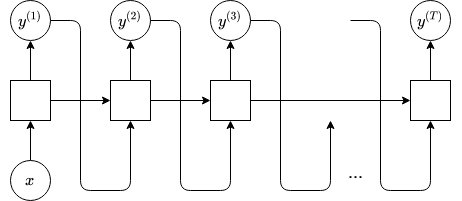
\includegraphics[width=0.8\textwidth]{onetomany}
  \caption{Red recurrente con arquitectura \textit{one-to-many}}
  \label{fig:onetomany}
\end{figure}

\begin{figure}[htpb]
\centering
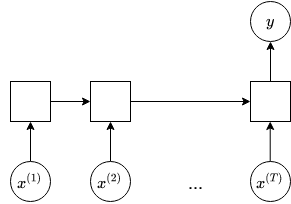
\includegraphics[width=0.6\textwidth]{manytoone}
\caption{Red recurrente con arquitectura \textit{many-to-one}}
\label{fig:manytoone}
\end{figure}

\begin{figure}[htpb]
  \centering
  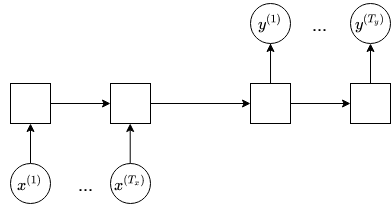
\includegraphics[width=0.75\textwidth]{encoderdecoder}
  \caption{Red recurrente con arquitectura codificador-decodificador}
  \label{fig:encoderdecoder}
\end{figure}


\subsection{Redes recurrentes bidireccionales}\label{rnn-bidirec}

Las redes recursivas mencionadas hasta el momento, en el instante $t$, solo capturan información de las entradas pasadas y presentes, $\textbf{x}^{(1)},...,\textbf{x}^{(t-1)},\textbf{x}^{(t)}$. En muchas aplicaciones, sin embargo, la salida deseada no depende solo de las posiciones previas en la secuencia, sino de la secuencia de entrada completa. Podemos encontrar un ejemplo de esto en el reconocimiento de voz. La correcta interpretación de un fonema puede depender de los siguientes, o incluso de las siguientes palabras. Si hay varias interpretaciones de una palabra, ambas acústicamente plausibles, puede ser necesario recurrir a la información que se tiene del futuro y del pasado para elegir la más correcta. Las redes neuronales recurrentes bidireccionales (RNNs bidireccionales) se crearon para afrontar este tipo de problemas.

Las redes recurrentes bidireccionales combinan dos redes recurrentes, una que avanza hacia adelante en el tiempo, desde el principio hasta al final de la secuencia de entrada, y otra que se mueve en dirección contraria, desde el final de la secuencia de entrada hasta su principio. La salida de cada instante dependerá de los estados ocultos de ambas subredes. De esta manera las unidades de salida producen una representación que depende del pasado y del futuro, y que es más sensible a entradas cercanas en el tiempo.

\begin{figure}[htpb]
  \centering
  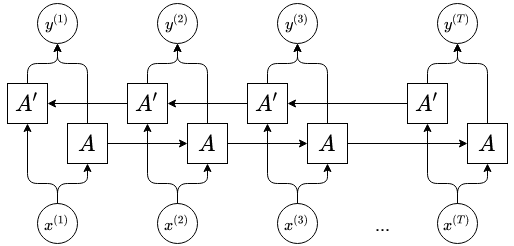
\includegraphics[width=1\textwidth]{bidirectional}
  \caption{Red recurrente bidireccional}
  \label{fig:bidirectional}
\end{figure}

\subsection{Redes recurrentes profundas}\label{rnn-deep}

Podemos clasificar las operaciones que realizan la mayoría de redes neuronales profundas en tres categorías de parámetros y sus transformaciones asociadas:

\begin{enumerate}
\item desde la entrada hasta el estado oculto,
\item desde el estado oculto previo hasta el siguiente estado oculto y
\item desde el estado oculto a la salida.
\end{enumerate}

Hasta ahora cada uno de estos bloques ha estado asociado a una única matriz de pesos, es decir, realiza una transformación que puede ser representada por una única capa de una red prealimentada profunda. La evidencia experimental (\cite{graves2013speech}, \cite{pascanu2013construct}) sugiere que puede ser beneficioso introducir una mayor profundidad en cada una de las categorías. Si se piensa en la capacidad de representación, aumentar la profundidad resulta beneficioso. Sin embargo puede ser contraproducente para el aprendizaje, ya que hace la optimización más difícil.

La profundidad de una red recurrente puede aumentarse añadiendo capas ocultas, que pueden introducirse como capas ocultas recurrentes o como capas previas o posteriores a la capa o capas recurrentes. La estructura de una red recurrente profunda queda reflejada en la \autoref{fig:deeprecurrent}.

\begin{figure}[htpb]
  \centering
  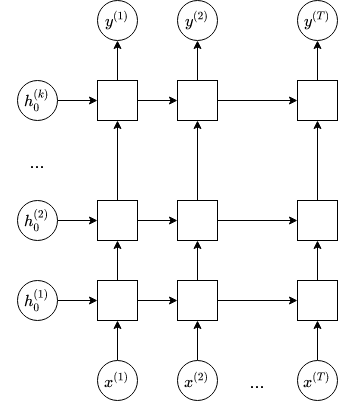
\includegraphics[width=0.6\textwidth]{deeprecurrent}
  \caption{Red recurrente profunda}
  \label{fig:deeprecurrent}
\end{figure}

\section{Dependencia a largo plazo}

Para muchas de las aplicaciones que hemos visto hasta ahora de las redes neuronales recurrentes es importante que el modelo conserve cierta información a través del tiempo hasta instantes lejanos. Cuando los grafos de los modelos usados se vuelven muy profundos, y especialmente en el caso de las redes recurrentes en las que la profundidad consiste en la aplicación múltiples veces de la misma operación, surgen problemas en el aprendizaje. En esta sección se describe el motivo de estos problemas y algunas propuestas para su afrontamiento.

\subsection{Problemas del gradiente en redes recurrentes}

El problema clave en el aprendizaje de dependencias a largo plazo es que el gradiente, propagado a través de gran cantidad de etapas, tiende a desvanecerse hacia valores casi nulos en la mayoría de los casos o, más raramente pero siendo más dañino para la optimización, a explotar hacia valores muy grandes. Estos son los conocidos como \textit{vanishing gradient problem} y \textit{exploding gradient problem}.

Las redes recurrentes se basan en la composición de la misma función, una vez cada paso. La composición sucesiva de funciones no lineales puede resultar en un comportamiento extremadamente no lineal, con una gran mayoría de valores con derivada casi nula, algunos valores con derivadas muy grandes y gran cantidad de alteraciones entre crecimiento y decrecimiento.

En particular, la composición empleada por las redes recurrentes neuronales es parecida a la multiplicación de matrices. Podemos tomar un ejemplo simplificado con $$\textbf{h}^{(t)} = \textbf{W}^T\textbf{h}^{(t-1)},$$ una red recurrente muy simple con función de activación lineal y sin entrada. En este caso, la aplicación del paso $t$-ésimo consiste en multiplicar la matriz de pesos \textbf{W} traspuesta con el estado anterior. Por lo tanto llegar al estado $t$-ésimo es, simplemente, aplicar esta operación $t$ veces sobre el estado inicial, $$\textbf{h}^{(t)} = \left( \textbf{W}^t \right)^T \textbf{h}^{(0)}.$$ Suponiendo $\textbf{W}$ diagonalizable, con $$ \textbf{W} = \textbf{Q}\textbf{A}\textbf{Q}^T, $$ con $\textbf{Q}$ ortogonal, podemos expresar $$\textbf{h}^{(t)} = \textbf{Q}^T\textbf{A}^t\textbf{Q}\textbf{h}^{(0)}. $$

Los valores propios están elevados a $t$, lo que produce que aquellos con valor propio menor que $1$ tenderán a desvanecerse hacia 0 y los que tengan valor propio mayor que $1$ a explotar con valores muy grandes. Por tanto, cualquier componente de $\textbf{h}^{(0)}$ que no esté alineada con valores propios grandes será descartada.

A continuación se exponen algunas alternativas a las redes recurrentes cuyo objetivo es evitar problemas con el gradiente y memorizar así dependencias a largo plazo.

\subsection{Redes recurrentes con puertas}

Los modelos que han demostrado ser más efectivos en aplicaciones prácticas para el uso de secuencia son las redes neuronales recursivas con puertas (\textit{gated RNNs}). Estos se basan en la idea de crear caminos a lo largo del tiempo cuyo gradiente no se desvanezca ni explote. A través de estos las redes recursivas con puertas podrán acumular información. Cuándo la información se almacena y se descarta será también aprendido por la red. Existen dos alternativas principales, modelos con memoria larga a corto plazo (\textit{long-short term memory, LSTM}), y las redes basadas en unidades recurrentes con puertas (\textit{gated recurrent unit, GRU}).

\subsubsection{LSTM}\label{lstm}

Las unidades de las redes neuronales simples son sustituidas por estructuras más complejas, a las que se llama bloques LSTM. Así, una red con LSTM tiene la misma forma de cadena de una RNN, pero utilizando estas nuevas estructuras cuyo comportamiento está dirigido a conservar información en el largo plazo~\cite{hochreiter1997long}.

\begin{figure}[htpb]
  \centering
  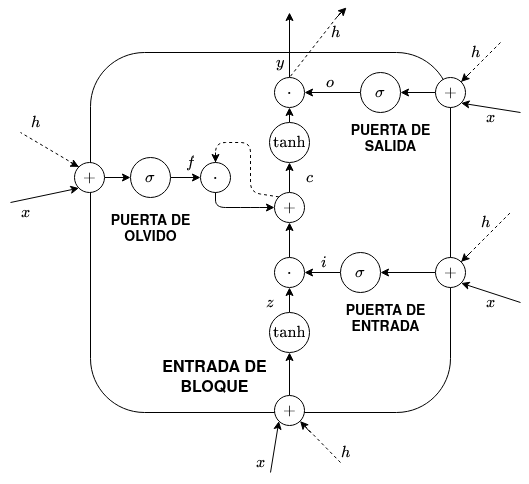
\includegraphics[width=1\textwidth]{LSTM}
  \caption{Bloque LSTM. Las líneas discontinuas representan conexiones con retardo en el tiempo}
  \label{fig:LSTM}
\end{figure}

La estructura de una célula es la representada en la gráfica \autoref{fig:LSTM}. La adición clave es una celda de memoria en cada bloque, $\textbf{c}^{(t)}$. La información que se se almacena desde la entrada y el estado oculto en la celda y que se entrae de la misma hacia la salida viene filtrada por diferentes puertas, unidades con su correspondiente función de activación.

El primer paso es decidir qué información se elimina de la celda. Esta decisión se realiza mediante la puerta de olvido, que contiene una unidad sigmoidal cuyas entradas son el estado oculto anterior $ \textbf{h}^{(t-1)}$ y la entrada del bloque $\textbf{x}^{(t)}$. Su salida $\textbf{f}^{(t)}$, entre $0$ y $1$, señala con qué intensidad se mantiene la información de la celda.

El siguiente paso es decidir qué nueva información se almacena en la celda. Se realiza en dos etapas. En la primera una unidad sigmoidal llamada puerta de entrada decide qué valores se actualizarán. Después una unidad $\tanh$ crea un vector con los nuevos datos candidatos $\textbf{z}^{(t)}$, que serán sumados a la celda. Por último se combinan estos dos pasos, multiplicando coordenada a coordenada, para definir finalmente la actualización de la celda.

A continuación se actualiza el estado anterior de la celda. Basta multiplicar coordenada a coordenada el estado anterior por el vector obtenido en la puerta de olvido y sumarle el vector obtenido en la puerta de entrada.

Por último se procesa la salida, que será una versión filtrada de la celda de memoria utilizando la entrada y el estado oculto anterior. El estado oculto y la entrada son transformadas por una unidad sigmoidal. El estado actual de la célula pasa por una unidad de $\tanh$ y se multiplica componente a componente su salida con la de la puerta de salida.

Podemos resumir el modelo en las siguientes ecuaciones, donde $\odot$ representa el producto componente a componente~\cite{greff2016lstm}:

\begin{itemize}
\item Entrada de bloque: $\textbf{z}^{(t)} = \tanh(\textbf{W}_z \textbf{x}^{(t)} +  \textbf{R}_z \textbf{h}^{(t-1)}  + \textbf{b}_z)$
\item Puerta de entrada: $\textbf{i}^{(t)} = \sigma(\textbf{W}_i\textbf{x}^{(t)} + \textbf{R}_i \textbf{h}^{(t-1)} + \textbf{b}_i)$
\item Puerta de olvido: $\textbf{f}^{(t)} = \sigma(\textbf{W}_f \textbf{x}^{(t)} + \textbf{R}_f\textbf{h}^{(t-1)} + \textbf{b}_f)$
\item Celda: $\textbf{c}^{(t)} = \textbf{z}^{(t)}\odot \textbf{i}^{(t)} + \textbf{c}^{(t-1)} \odot \textbf{f}^{(t)}$
\item Puerta de salida: $\textbf{o}^{(t)} = \sigma(\textbf{W}_o \textbf{x}^{(t)} + \textbf{R}_o \textbf{h}^{(t-1)} + \textbf{b}_o)$
\item Salida de bloque: $\textbf{h}^{(t)} = \tanh (\textbf{c}^t) \odot \textbf{o}^{(t)}$
\end{itemize}

donde $\textbf{W}_z$, $\textbf{W}_i$, $\textbf{W}_f$, $\textbf{W}_o$ son las matrices de pesos para la entrada en cada una de las unidades, $\textbf{R}_z$, $\textbf{R}_i$, $\textbf{R}_f$, $\textbf{R}_o$ las matrices de pesos para los estados ocultos previos y $\textbf{b}_z$, $\textbf{b}_i$, $\textbf{b}_f$, $\textbf{b}_o$ los respectivos vectores de sesgos.

Sobre el bloque LSTM visto hasta ahora pueden introducirse varias modificaciones. La más popular es la que introduce conexiones de mirilla (\textit{peephole connections})~\cite{gers2000recurrent}, mediante las cuales se conecta el estado de la celda de memoria con cada una de las unidades de las puertas. Estas conexiones pueden añadirse a todas las puertas o solo a algunas.

\begin{figure}[htpb]
  \centering
  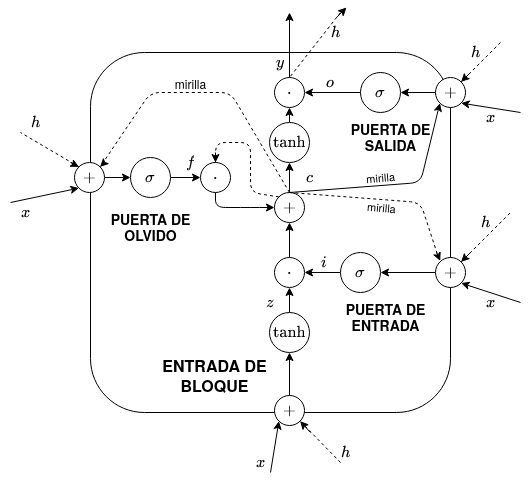
\includegraphics[width=1\textwidth]{LSTM-peephole}
  \caption{Bloque LSTM con conexiones de mirilla. Las líneas discontinuas representan conexiones con retardo en el tiempo}
  \label{fig:LSTM-peephole}
\end{figure}

\subsubsection{GRU}

Una variación que surge de la simplificación de las celdas LSTM vistas anteriormente son las unidades recurrentes con puertas (\textit{gated  recurrent unit}, GRU)~\cite{cho2014learning}. La principal diferencia es que combina la puerta de entrada y la puerta de olvido en una sola unidad, la puerta de actualización (\textit{update gate}). Tampoco diferencia entre estado oculto y celda de memoria, por lo que no es necesario el uso de una puerta de salida. A continuación se describe su funcionamiento detalladamente.

\begin{figure}[htpb]
  \centering
  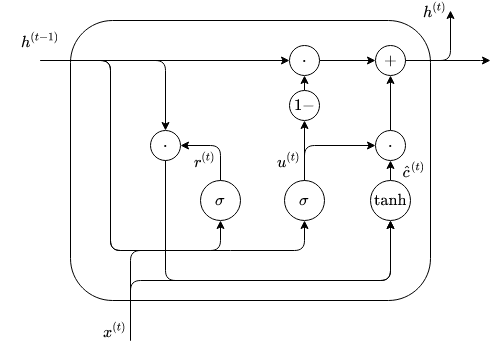
\includegraphics[width=0.9\textwidth]{gru}
  \caption{Bloque GRU}
  \label{fig:gru}
\end{figure}


Primeramente el estado previo anterior $\textbf{h}^{(t-1)}$ y la entrada actual $\textbf{x}^{(t)}$ son filtrados a través de la puerta de relevancia, que normalmente es una unidad sigmoidal. Su salida $\textbf{r}^{(t)}$ indica cómo de relevante es el estado oculto previo.

A continuación se calcula el valor $\textbf{u}^{(t)}$ de la puerta de actualización mediante otra unidad sigmoidal. El valor $1 - \textbf{u}^{(t)}$ sustituye al que en LSTM correspondería a la salida de la puerta de olvido.

Los datos candidatos se calculan, por tanto, aplicando una unidad $\tanh$ a la multiplicación componente a componente de la salida de la puerta de relevancia, $\textbf{r}^{(t)}$, y la entrada actual, $\textbf{x}^{(t)}$. La actualización del estado oculto se realiza entonces sumando la multiplicación componente a componente de los datos candidatos por la salida de la puerta de actualización con el producto componente a componente de $1 - \textbf{u}^{(t)}$ con el valor oculto anterior.

Podemos resumir el modelo en las siguientes ecuaciones, donde $\odot$ representa el producto componente a componente:

\begin{itemize}
\item Puerta de relevancia: $ \textbf{r}^{(t)} = \sigma(\textbf{W}_r\textbf{x}^{(t)} + \textbf{R}_r \textbf{h}^{(t-1)} + \textbf{b}_r)$
\item Puerta de actualización: $ \textbf{u}^{(t)} = \sigma(\textbf{W}_u\textbf{x}^{(t)} + \textbf{R}_u \textbf{h}^{(t-1)} + \textbf{b}_u)$
\item Candidato a estado oculto: $\hat{\textbf{c}}^{(t)} = \tanh(\textbf{W}_c\textbf{x}^{(t)} + \textbf{R}_c( \textbf{r}^{(t)} \odot \textbf{h}^{(t-1)}) + \textbf{b}_c)$
\item Salida: $\textbf{h}^{(t)} = (1- \textbf{u}^{(t)}) \odot \textbf{h}^{(t-1)} + \textbf{z}^{(t)} \odot \hat{\textbf{c}}^{(t)}$
\end{itemize}

donde $\textbf{W}_r$, $\textbf{W}_u$, $\textbf{W}_c$ son las matrices de pesos para la entrada en cada una de las unidades, $\textbf{R}_r$, $\textbf{R}_u$, $\textbf{R}_c,$ las matrices de pesos para los estados ocultos previos y $\textbf{b}_r$, $\textbf{b}_u$, $\textbf{b}_c$ los respectivos vectores de sesgos.


\endinput
%------------------------------------------------------------------------------------
% FIN DEL CAPÍTULO.
%------------------------------------------------------------------------------------

% !TeX root = ../libro.tex
% !TeX encoding = utf8

\chapter{Aprendizaje de características}

La efectividad de los métodos de aprendizaje automático depende en gran medida de la representación de los datos utilizada. La obtención de una buena representación es crucial en el proceso de aprendizaje. Dicha tarea es una de las que más tiempo consumen en cualquier proyecto de esta área~\cite{domingos2012few}. El desarrollo de técnicas que permitan la obtención de buenas representaciones automáticamente se ha convertido en un importante campo dentro del aprendizaje automático. A este conjunto de técnicas se le denomina aprendizaje de características o de representación.~\cite{bengio2013representation}.

Obtener representaciones mejores para la aplicación de técnicas de aprendizaje no es el único motivo para la aplicación del aprendizaje de características. En muchas aplicaciones la obtención de características es la meta en sí. Algunos ejemplos de esto son la representación de documentos en códigos binarios compactos que faciliten su búsqueda~\cite{salakhutdinov2009semantic}, compresión de imágenes minimizando la pérdida de información~\cite{theis2017lossy}, la transformación del dominio de un problema a otro diferente~\cite{deng2013sparse} o la generación de imágenes restauradas a partir de versiones distorsionadas~\cite{xie2012image}.

En el caso de este trabajo se aplica esta idea a la manipulación y generación de melodías musicales. Estas son datos de naturaleza compleja, difíciles de manejar de forma rápida y efectiva, y más aún con la inmediatez que requiere una interpretación en directo. Utilizaremos melodías monofónicas de dos compases de 4/4, es decir, como máximo una nota suena a la vez y hay cuatro pulsos por compás. Supongamos además, con afán de simplificación, que la máxima subdivisión posible para dichas melodías es la semicorchea (un cuarto de pulso) e ignoremos el tempo al que se interpreta la secuencia y el volumen. Si suponemos que las notas diferentes posibles son las 88 que tienen los pianos actuales y que en cada pulso podemos tocar una de las 88 teclas, levantar la tecla que se venía tocando o realizar un silencio, esto nos deja 90 posibles acciones para cada semicorchea. Necesitaríamos entonces 7 bits por semicorchea para su cifrado, y tenemos 32 semicorcheas por melodía. Explorar todas las posibilidades bit a bit es una tarea intratable y la mayoría de melodías obtenidas serían incoherentes ~\cite{roberts2018learning}.

El objetivo será por tanto obtener una representación de estas melodías fácil de manipular por parte del artista, que permita un acercamiento diferente a la composición y la interpretación. Para ello será clave la extracción de representaciones de baja dimensionalidad.

\section{Selección de características}
El precedente para la extracción de características se encuentra en la selección de características para problemas de aprendizaje automático. En los últimos años del número de características utilizadas ha crecido desde las pocas decenas hasta las miles o decenas de miles~\cite{guyon2003introduction}. Con este crecimiento surge también la necesidad de seleccionar aquellas características más útiles para la tarea que se pretende afrontar.

La selección de características consiste en seleccionar un subconjunto de entre las características disponibles para mejorar la tarea de aprendizaje. Existen muchos beneficios potenciales que pueden derivarse de esta acción: facilitar la visualización y entendimiento de los datos, disminución de los recursos computacionales necesarios, tanto en espacio de memoria para almacenaje de datos como en tiempo de cómputo en el entrenamiento y predicción, o evitar la maldición de la dimensionalidad (\textit{the curse of dimensionality}) que obstaculiza o imposibilita el aprendizaje cuando se cuenta con pocos ejemplos y un número de características elevado~\cite{beyer1999nearest}.

Un primer acercamiento a la selección de características consiste en la jerarquización de variables utilizando alguna métrica del valor de cada variable para el aprendizaje y descartando las menos útiles. Es una técnica ampliamente usada por su simplicidad, escalabilidad y buen desempeño empírico, pero presenta un problema importante. La mayoría de las veces la utilidad de una variable no puede juzgarse individualmente, y la inclusión de variables que resultan redundantes por sí solas pueden producir una mejora significativa de los resultados por su relación con otras.

Como respuesta a este hecho surgen métodos que no tratan de seleccionar características individualmente, sino conjuntos de características. De entre estos podemos distinguir tres categorías:

\begin{itemize}

  \item Métodos de filtro: seleccionan el subconjunto de características como paso de preprocesamiento de datos, independientemente del predictor elegido.
  \item Métodos de envoltura: utilizan el desempeño de un algoritmo de aprendizaje automático para medir la utilidad del subconjunto seleccionado. Su alto coste computacional implica que una búsqueda exhaustiva sea imposible en la práctica, por lo que la estrategia de búsqueda utilizado es clave en este tipo de métodos.
  \item Métodos integrados: realizan la selección de características durante el aprendizaje y son específicos del algoritmo de aprendizaje usado.

\end{itemize}

\section{Extracción de características}

Frente a la selección de entre las características ya existentes aparece una perspectiva diferente: la creación de nuevas representaciones a partir de la existente, no solo mediante la selección sino mediante la generación de nuevas características a través de transformaciones de las iniciales. Surge no solo con la intención de generar representaciones más eficientes para el aprendizaje, sino también más comprensibles y fáciles de manejar.

Puede pasar que todas las características de los datos sean relevantes, y aún así la dimensionalidad de los mismos sea todavía demasiado elevada. Descubrir las dependencias entre las características puede permitir reducir dicha dimensionalidad. Cuando dos características están altamente correladas, conocer información sobre una implica conocer información sobre la otra. En lugar de eliminar arbitrariamente una de estas características, una manera de reducir la dimensionalidad es obtener una  representación a partir de una transformación de dichas características. Esta perspectiva viene motivada por el hecho de que las dependencias entre variables pueden ser muy complejas, y eliminar una de ellas puede resultar en perder parte de la información que ambas comunican~\cite{lee2007nonlinear}.

El nuevo conjunto de características por lo general debe tener un número menor de variables pero debe preservar la información del conjunto inicial. Se buscan por tanto transformaciones de las variables con unas propiedades tales que se asegure que la transformación no altera la información que contenían las variables iniciales, solo su representación.

Estas transformaciones pueden intentar cumplir dos objetivos diferentes. El primero, y más simple, es detectar y eliminar dependencias. Para ello la transformación debe reducir el número de variables. El segundo, y más complejo, es recuperar las variables latentes, esto es, aquellas que son el origen de las observadas, pero que no pueden medirse directamente.

La construcción de una representación nueva podría considerarse una tarea muy específica del dominio de la información que se trata, y puede ser la manera de introducir conocimiento específico sobre dicho dominio. Sin embargo, se han desarrollado gran cantidad de técnicas genéricas para la construcción de nuevas representaciones.
En esta sección se repasan algunas de ellas. Se explicarán algunas de las técnicas tradicionales para después hacer especial hincapié en aquellas para las que se aplica aprendizaje profundo.

\subsection{Técnicas tradicionales de extracción de características}

Podemos separar las técnicas entre aquellas que realizan transformaciones lineales de los datos de entrada y las que realizan transformaciones no lineales. De entre las técnicas lineales la más extendida es el análisis de componentes principales.

% Mencionar: (Lineales: PCA, LDA. No lineales: Isomap, LLE)

El análisis de componentes principales (\textit{principal component analysis}, PCA) se base en la asunción de que las $D$ variables observadas, expresadas en el vector aleatorio $\textbf{Y} = (Y_1,...,Y_D)^T$ son el resultado de una transformación lineal $\textbf{W}$ de variables $P$ latentes desconocidas, $\textbf{X} = (X_1,...,X_M)^T$: $$\textbf{Y} = \textbf{W}\textbf{X}.$$ Se asume también que todas las variables latentes tienen una distribución normal, y que la transformación $\textbf{W}$ es un cambio de ejes, es decir, que sus columnas son ortogonales entre sí y tienen norma unitaria. En definitiva, $\textbf{W} \in \mathcal{M}_{D \times P}$, con $\textbf{W}^T\textbf{W} = \textbf{I}_P$. Por último, pero menos restrictivo, PCA asume que las variables observadas ${y}$ y las variables latentes $\textbf{x}$ están centradas, es decir, $E[\textbf{X}] = 0_D$ y $E[\textbf{Y}] = 0_P$.

A partir de estas condiciones se pretende obtener la dimensión $P$ y la transformación $\textbf{W}$ a partir de un conjunto de $N$ observaciones del vector aleatorio $\textbf{Y}$, que pueden expresarse como una matriz $$Y = [\textbf{Y}^{(1)},...,\textbf{Y}^{(N)}].$$

Si asumimos que las variables de $\textbf{X}$ son incorreladas, es decir, que la matriz de covarianzas $Cov(\textbf{X}) = E[\textbf{X}\textbf{X}^T]$ es diagonal. Tras la transformación por $\textbf{W}$ las variables de $\textbf{y}$ sí estarán correladas, y su matriz de covarianzas no será diagonal. El objetivo de PCA es obtener las $P$ variables incorreladas de $\textbf{X}$ a través de las de $\textbf{Y}$. Podemos expresar la matriz de covarianzas de $\textbf{Y}$ como $$Cov(\textbf{Y}) = E[\textbf{Y}\textbf{Y}^T] = E[\textbf{W}\textbf{X}\textbf{X}^T\textbf{W}^T] = \textbf{W}E[\textbf{X}\textbf{X}^T]\textbf{W}^T = \textbf{W}Cov(\textbf{X})\textbf{W}^T.$$ Como $\textbf{W}^T\textbf{W} = \textbf{I}$, multiplicando a la izquierda por $\textbf{W}^T$ y a la derecha por $\textbf{W}$ obtenemos $$Cov(\textbf{X}) = \textbf{W}^TCov(\textbf{Y})\textbf{W}. $$ Podemos entonces factorizar la matriz Cov(\textbf{Y}), que por ser simétrica es diagonalizable, como $$ Cov(\textbf{Y}) = \textbf{V}\textbf{A}\textbf{V}^T,$$ donde \textbf{V} es una matriz de vectores propios normalizados $\textbf{v}_d$ y $\textbf{A}$ es una matriz diagonal con los valores propios asociados $\lambda_d$, en orden descendiente. Como la matriz de covarianzas es simétrica y semidefinida positiva los vectores propios son ortogonales y los valores propios son reales no negativos. Sustituyendo en la expresión de $Cov(\textbf{X})$ obtenemos $$Cov(\textbf{X}) = \textbf{W}^T\textbf{V}\textbf{A}\textbf{V}^T\textbf{W},$$ donde, en el caso ideal en el que todas las hipótesis son respetadas y las observaciones no tienen ruido, solo los primeros $P$ valores propios en $\textbf{A}$ son positivos, siendo el resto nulos. Tomamos entonces los vectores propios asociados a estos $P$ valores, $$\textbf{W} = \textbf{V}\textbf{I}_{D \times P},$$ obteniendo así $$Cov(\textbf{X}) = \textbf{I}_{P \times D}\textbf{A}\textbf{I}_{D \times P}.$$ Esto significa que los valores propios en $\textbf{A}$ se corresponden con las varianzas de las variables latentes.

En la práctica los datos observados serán ruidosos y por tanto todos los valores propios de $Cov(\textbf{Y})$ serán mayores que cero, por lo que la elección de las $P$ columnas en $\textbf{V}$ es más complicada. Si las variables latentes tienen varianzas mayores que el ruido, basta tomar los vectores correspondientes a los mayores valores propios.

Desde un punto de vista geométrico, las columnas de $\textbf{V}$ indican las direcciones en $\mathbb{R}^D$ sobre las que se extiende el subespacio de las variables latentes. Si llamamos a estas columnas componentes, la elección de las columnas asociadas a las mayores varianzas es la elección de las componentes principales.

En una situación real la covarianza de $\textbf{Y}$ no es conocida, pero puede ser aproximada mediante la covarianza de la muestra: $$Cov(Y) = \frac{1}{N}YY^T.$$

Otra técnica lineal muy extendida es el análisis discriminante lineal. En este caso se trata de un método supervisado para datos clasificados. Genera una representación de los datos con una dimensión menor que respeta la estructura de clases y maximiza la separación entre las mismas. Es habitual aplicarla tras PCA~\cite{ye2005two}.

En cuanto a las técnicas que utilizan transformaciones no lineales, el escalamiento multidimensional (\textit{multidimensional scaling}, MDS) es una técnica que además sirve como base para otros algoritmos. Consiste en encontrar nuevas coordenadas en un espacio de menor dimensión manteniendo las distancias relativas entre los datos de manera lo más fiel posible. Isomap se basa en MDS, extendiéndolo para encontrar coordenadas que describan los verdaderos grados de libertad de los datos mientras que se preservan las distancias entre puntos. Por último la máquina de Boltzmann restringida (\textit{restricted boltzmann machine}, RMB) es un modelo que cuenta con una capa oculta y una visible. Están definidas por una distribución de probabilidad conjunta determinada por una función de energía. Son una alternativa para la inicialización de \textit{autoencoder} por capas, que veremos a continuación.

\subsection{Autoencoder}

Los \textit{autoencoder} (AE) son redes neuronales con una estructura simétrica, entrenados para reconstruir la entrada en la salida. La capa central representa la codificación de los datos de entrada. Por tanto, en este caso el interés no se encuentra en la salida de la red sino en la codificación obtenida mediante la misma. El objetivo del \textit{autoencoder} es obtener una representación de los datos de entrada con determinadas características, que estarán determinadas por la arquitectura de la red. Podemos por tanto considerar la estructura básica reflejada en \autoref{fig:basic-ae}: la entrada $\textbf{x}$ que se aplica en la codificación $\textbf{h}$ mediante el codificador (\textit{encoder}), representado por $f$, y la reconstrucción $\textbf{r}$, obtenida a partir de $\textbf{y}$ mediante el decodificador (\textit{decoder}), representado por $g$~\cite{goodfellow2016}.

\begin{figure}[htpb]
  \centering
  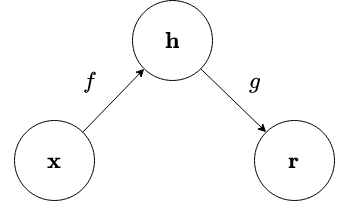
\includegraphics[width=0.6\textwidth]{basic-ae}
  \caption{Estructura básica de un \textit{autoencoder}}
  \label{fig:basic-ae}
\end{figure}

El \textit{autoencoder} más básico es una red prealimentada profunda con esta estructura. Puesto que se copia la entrada $\textbf{x}$ en la salida $\textbf{r}$, ambas tendrán la misma dimensión. La codificación $\textbf{y}$ es variable, y puede tener una dimensión menor o mayor en función de las propiedades deseadas en la representación de los datos de entrada. Tanto el codificador como el decodificador pueden tener tantas capas como sean necesarias, normalmente dispuestas de manera simétrica. Un ejemplo de red prealimentada profunda de esta forma puede observarse en la \autoref{fig:autoencoder}.

\begin{figure}[htpb]
  \centering
  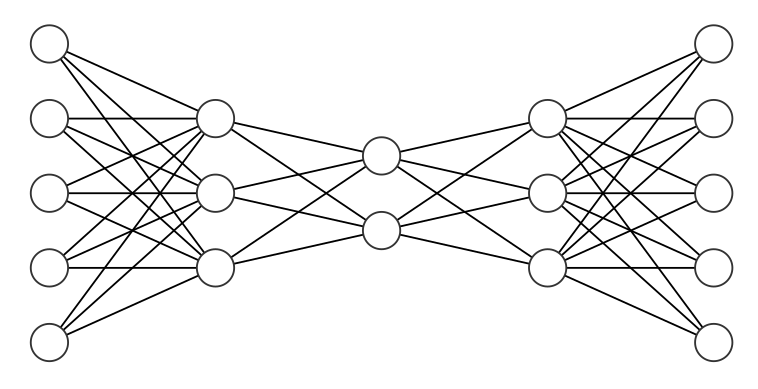
\includegraphics[width=0.8\textwidth]{autoencoder}
  \caption{Estructura de un \textit{autoencoder} como red prealimentada profunda}
  \label{fig:autoencoder}
\end{figure}

\subsubsection{Arquitecturas}

Los diferentes tipos de \textit{autoencoders} pueden ser clasificados según múltiples criterios. En este apartado se repasan las diferentes estructuras que puede tomar la red. Todas ellas son simétricas, con el codificador y el decodificador teniendo el mismo número de capas y de unidades en cada capa, en orden inverso. Puede considerarse que el codificador empieza en la entrada y tiene su salida en la codificación, que es la entrada del decodificador. La salida de este es la reconstrucción. Por tanto ambas estructuras comparten la capa de codificación. En función de las dimensiones de esta capa podemos considerar dos tipos de red:

\begin{itemize}
\item Incompleto (\textit{undercomplete}): la capa de codificación tiene dimensión menor que la de la entrada (y por tanto también que la salida). El menor número de unidades supone una restricción en la red, por lo que durante el entrenamiento el \textit{autoencoder} aprenderá una representación más compacta de la entrada. Cuando se tiene esta estructura la capa de codificación suele llamarse cuello de botella.
\item Sobrecompleto (\textit{overcomplete}): la capa de codificación tiene una dimensión igual o mayor a la de la entrada. Puede permitir que el \textit{autoencoder} aprenda la función identidad para copiar la entrada en la salida, por lo que suelen aplicarse otras restricciones. Mediante estas puede obtenerse también una representación compacta de los datos.
\end{itemize}

Además del número de unidades por capa, también pueden clasificarse los \textit{autoencoders} según la cantidad de capas que tienen. Así, podemos distinguir dos cateogrías:

\begin{itemize}
\item Superficial (\textit{shallow}): cuenta solamente con las capas de entrada, codificación y salida. Es la estructura más simple posible, pues tiene una única capa oculta, la capa de codificación.
\item Profundo (\textit{deep}): tiene más de una capa oculta. Puede ser entrenado capa a capa como si se tratara de varios \textit{autoencoders} superficiales superpuestos o como una única red profunda, como se explica en la \autoref{entrenamiento-ae}.
\end{itemize}

\begin{figure}
    \centering
    \begin{minipage}{0.45\textwidth}
        \centering
        
\includegraphics[width=1.1\textwidth]{undercomplete-shallow}
        \caption{\textit{Autoencoder} incompleto superficial}
    \end{minipage}\hfill
    \begin{minipage}{0.45\textwidth}
        \centering
        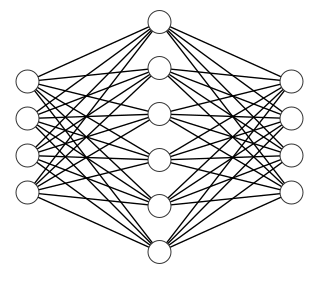
\includegraphics[width=1.1\textwidth]{overcomplete-shallow}
        \caption{\textit{Autoencoder} sobrecompleto superficial}
    \end{minipage}
\end{figure}

\begin{figure}
    \centering
    \begin{minipage}{0.45\textwidth}
        \centering
        
\includegraphics[width=1.2\textwidth]{undercomplete-deep}
        \caption{\textit{Autoencoder} incompleto profundo}
    \end{minipage}\hfill
    \begin{minipage}{0.45\textwidth}
        \centering
        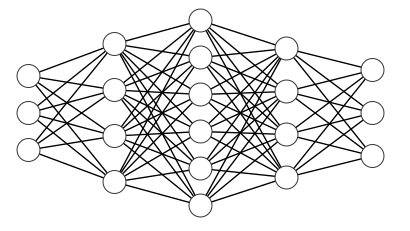
\includegraphics[width=1.2\textwidth]{overcomplete-deep}
        \caption{\textit{Autoencoder} sobrecompleto profundo}
    \end{minipage}
\end{figure}

\subsubsection{Funciones de activación más comunes}

Las unidades de activación generalmente utilizadas en los \textit{autoencoder} son las ya vistas en \autoref{unidades-ocultas}. Cuando se utilizan unidades de activación lineal con una sola capa oculta de $k$ unidades y se minimiza el error cuadrático medio, el modelo es equivalente a obtener las $k$ componentes principales mediante PCA.

Las unidades ReLU, muy utilizadas en muchos modelos de aprendizaje profundo, pueden resultar menos útiles para los \textit{autoencoder}. Puesto que su salida es nula para todos los valores negativos dificultan el proceso de reconstruir la entrada en la salida. Existe una alternativa reciente, las unidades lineales exponenciales escaladas (\textit{Scaled Exponential Linear Units}, SELU)~\cite{klambauer2017self}, cuya función de activación es

$$g(\textbf{z})_i = \lambda \left\{ \begin{array}{lcc}
             \alpha (e^x - 1) &   si  & x \leq 0
             \\ x &  si & x > 0
             \end{array}
   \right.,$$
con $\lambda > 1$.

\begin{figure}[htpb]
  \centering
  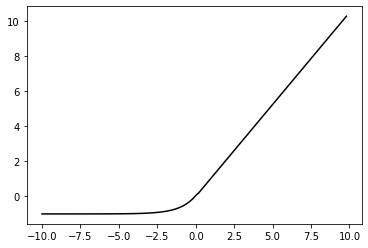
\includegraphics[width=0.6\textwidth]{selu}
  \caption{Gráfica de la función de activación de una SELU}
  \label{fig:selu}
\end{figure}

Es por esto que, en general, las funciones de activación más usadas son las sigmoides, tanto la función logística como la tangente hiperbólica.

\subsubsection{Función de coste}

La función de coste $J(W,b;S)$ del \textit{autoencoder} se calcula como la suma de las funciones de coste para cada elemento del conjunto de entrenamiento $L: \mathbb{R}^d \times \mathbb{R}^d \rightarrow \mathbb{R}$. Así, $$J(W,b;S) = \sum_{x \in S}L(x,(g \circ f)(x)),$$ donde $S$ es el conjunto de entrenamiento y $f$ y $g$ las funciones del codificador y decodificador respectivamente, determinadas por los pesos $W$ y los sesgos $b$. El objetivo será por tanto aprender $W$ y $b$ para minimizar $J$. La función $L$ suele tomarse como la log-verosimilitud negativa del ejemplo $x$ dada la salida $(g \circ f)(x)$.

\subsubsection{Entrenamiento}\label{entrenamiento-ae}

Para la optimización de \textit{autoencoders} pueden aplicarse los algoritmos vistos en la \autoref{optimizacion} basados en el descenso del gradiente como el descenso del gradiente estocástico y variantes como AdaGrad, RMSProp y Adam. Para el cálculo del gradiente se usa el algoritmo de propagación hacia atrás, también visto en la \autoref{back-propagation}.

Al igual que en los modelos de aprendizaje profundo del anterior capítulo, puede añadirse un término de regularización en la función de coste para evitar sobreajuste. Este término puede introducirse de distintas maneras, pero en general depende de los pesos para reducir su tamaño.

Conforme aumenta la profundidad de los \textit{autoencoders} el proceso de entrenamiento depende cada vez más de la inicialización de los pesos, ya que su número aumenta. Esta inicialización puede realizarse superponiendo sucesivos \textit{autoencoders} superficiales y entrenándolos capa a capa. Así, se comienza entrenando la primera capa oculta como si se tratara de un único \textit{autoencoder} superficial. La segunda capa se entrena de igual manera, tomando la salida de la primera capa como entrada, y así hasta haber completado todas las capas hasta llegar a la de codificación. Con esto se consigue una inicialización de los pesos para todas las capas del codificador. Las capas del decodificador se inicializan con la trasposición de los pesos de su capa simétrica. Finalmente puede realizarse un entrenamiento normal.

\subsection{Autoencoder variacional}

Los modelos descritos hasta el momento tienen su principal utilidad en generar representaciones más compactas de los datos de entrada. En contraposición, el \textit{autoencoder} variacional (\textit{variational autoencoder}, VAE) es un modelo generativo (\cite{kingma2013auto}, \cite{rezende2014stochastic}). Los modelos generativos aprenden una distribución de probabilidad de la que generar nuevos datos diferentes a los observados. Los \textit{autoencoder} son capaces de reconstruir datos codificados, pero no tienen por qué generar ejemplos válidos a partir de codificaciones arbitrarias. Los \textit{autoencoder} variacionales aprenden un modelo mediante el que pueden generarse nuevas instancias.

Consideremos el conjunto de datos $\textbf{X}$ = $\{\textbf{x}^{(i)}\}^N_{i=1}$ consistente en $N$ muestras de una variable aleatoria $X$. Asumimos que los datos son generados por un proceso aleatorio que implica una variable aleatoria no observada $Z$. El proceso consiste de dos pasos: primero un valor $\textbf{z}^{(i)}$ se genera de la distribución a priori $p_{\boldsymbol{\theta}^*}(\textbf{z})$, y después el valor $\textbf{x}^{(i)}$ se genera de una distribución condicional $p_{\boldsymbol{\theta}^*}(\textbf{x}|\textbf{z})$. Asumimos que la distribución a priori $p_{\boldsymbol{\theta}^*}(\textbf{z})$ y la distribución condicionada $p_{\boldsymbol{\theta}^*}(\textbf{x}|\textbf{z})$ vienen de familias paramétricas $p_{\boldsymbol{\theta}}(\textbf{z})$ y $p_{\boldsymbol{\boldsymbol{\theta}}}(\textbf{x}|\textbf{z})$. En concreto, en el caso del \textit{autoencoder} variacional, asumimos que la distribución a priori es una distribución normal multivariante de la forma $p_{\boldsymbol{\theta}}(\textbf{z}) = \mathcal{N}(\textbf{z};\mathbf{0},\textbf{I})$ y la distribución $p_{\boldsymbol{\theta}}(\textbf{x}|\textbf{z})$ una distribución normal multivariante, que actuará como decodificador.

Tanto el codificador como el decodificador toman la forma de redes neuronales que modelan distribuciones multivariantes normales con covarianza diagonal. En el caso del decodificador $$\log p(\textbf{x}|\textbf{z}) = \log \mathcal{N}(\textbf{x}; \boldsymbol{\mu},\boldsymbol{\sigma}^2\textbf{I}),$$ con $$\mu = \textbf{W}_2\textbf{h} + \textbf{b}_2,$$ $$\log \boldsymbol{\sigma}^2 = \textbf{W}_3\textbf{h} + \textbf{b}_3,$$ $$\textbf{h} = tanh(\textbf{W}_1\textbf{z} + \textbf{b}_1).$$ Así, $\{\textbf{W}_1, \textbf{W}_2, \textbf{W}_3, \textbf{b}_1, \textbf{b}_2, \textbf{b}_3\}$ son los pesos y sesgos de la red.

Utilizando este modelo hay que resolver dos problemas:

\begin{itemize}
\item Aproximar los parámetros $\boldsymbol{\theta}$ que rigen la distribución. Pueden ser de interés por sí mismos, para analizar un proceso natural, pero también permiten imitar la variable aleatoria oculta para generar nuevos datos parecidos a los reales.
\item Aproximar la distribución a posteriori de la variable latente $\textbf{z}$ dado el valor de $\textbf{x}$ y elegidos unos parámetros $\boldsymbol{\theta}$, $p_{\boldsymbol{\theta}}(\textbf{x}|\textbf{z})$. Con ello obtenemos la codificación de los datos en las variables latentes.
\end{itemize}

El principal inconveniente es que, a la hora de calcular la distribución a posteriori que usar en el codificador mediante la regla de Bayes $$ p_{\boldsymbol{\theta}}(\textbf{z}|\textbf{x}) = \frac{p_{\boldsymbol{\theta}}(\textbf{x}|\textbf{z})p_{\boldsymbol{\theta}}(\textbf{z})}{p_{\boldsymbol{\theta}}(\textbf{x})}$$ el cálculo de la integral de la distribución marginal $p_{\boldsymbol{\theta}}(\textbf{x}) = \int p_{\boldsymbol{\theta}}(\textbf{x},\textbf{z})d\textbf{z} = \int p_{\boldsymbol{\theta}}(\textbf{z})p_{\boldsymbol{\theta}}(\textbf{x}|\textbf{z})d\textbf{z}$ es intratable~\cite{kingma2019introduction}.

Para solucionarlo se introduce el modelo de reconocimiento $q_{\boldsymbol{\phi}}(\textbf{z}|\textbf{x})$, una aproximación de la verdadera distribución a posteriori $p_{\boldsymbol{\theta}}(\textbf{z}|\textbf{x})$. En este caso tomamos $$\log q_{\boldsymbol{\phi}}(\textbf{z}|\textbf{x}^{(i)}) = \log \mathcal{N}(\textbf{z};\boldsymbol{\mu}^{(i)},\boldsymbol{\sigma}^{2(i)}\textbf{I}),$$ donde la media y la desviación típica, $\boldsymbol{\mu}^{(i)}$ y $\boldsymbol{\sigma}^{(i)}$ son las salidas de la red neuronal del codificador.

\begin{figure}[htpb]
  \centering
  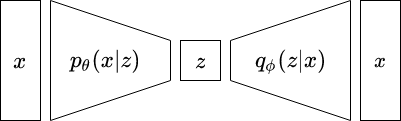
\includegraphics[width=0.6\textwidth]{vae}
  \caption{Estructura de un \textit{autoencoder} variacional}
  \label{fig:vae}
\end{figure}

\subsubsection{Función de coste}

Optimizando la función de coste se quiere conseguir que la aproximación $q_{\boldsymbol{\phi}}(\textbf{z}|\textbf{x})$ sea lo más cercana posible a la verdadera distribución a posteriori $p_{\boldsymbol{\theta}}(\textbf{z}|\textbf{x})$. Para ello debe introducirse una medida de la similitud entre dos funciones de distribución, la divergencia de Kullback-Leibler~\cite{kullback1997information}.

\begin{definicion}Dadas dos distribuciones de probabilidad P y Q sobre el mismo espacio de probabilidad, se define la \textit{divergencia de Kullback-Leibler} como $$D_{KL}(Q \parallel P) = E_Q \left[ \log \frac{Q(x)}{P(x)} \right].$$
\end{definicion}

\begin{proposicion}Dadas dos distribuciones de probabilidad P y Q sobre el mismo espacio de probabilidad, se cumple que $$D_{KL}(Q \parallel P) \geq 0.$$
\end{proposicion}\label{DKL-norm}

Realizamos también el cálculo de la divergencia entre dos distribuciones normales, que será útil para calcular la expresión concreta de la función de coste.

\begin{proposicion} Dadas las distribuciones de probabilidad  $p(\textbf{x}) = N(\textbf{x};\boldsymbol{\mu}_1, \boldsymbol{\Sigma}_1) $ y $q(\textbf{x}) = N(\textbf{x};\boldsymbol{\mu}_2, \boldsymbol{\Sigma}_2)$, ambas de dimensión $k$,
se cumple que $D_{KL}(p(\textbf{x}) \parallel q(\textbf{x})) = \frac{1}{2} \left( \log \frac{|\boldsymbol{\Sigma}_1|}{|\boldsymbol{\Sigma}_2|} - k + tr(\boldsymbol{\Sigma}_2^{-1}\boldsymbol{\Sigma}_1) + (\boldsymbol{\mu}_2 - \boldsymbol{\mu}_1)^T \boldsymbol{\Sigma}_2^{-1} (\boldsymbol{\mu}_2 - \boldsymbol{\mu}_1) \right).$\end{proposicion}

\begin{proof}
Comenzamos tomando el logaritmo de las funciones de densidad: $$ \log p(\textbf{x}) = -\frac{k}{2}\log(2 \pi) - \frac{1}{2} \vert \boldsymbol{\Sigma}_1\vert - \frac{1}{2}(\textbf{x} - \boldsymbol{\mu}_1)^T\boldsymbol{\Sigma}_1^{-1}(\textbf{x} - \boldsymbol{\mu}_1),$$ $$ \log p(\textbf{x}) = -\frac{k}{2}\log(2 \pi) - \frac{1}{2} \vert \boldsymbol{\Sigma}_2\vert - \frac{1}{2}(\textbf{x} - \boldsymbol{\mu}_2)^T\boldsymbol{\Sigma}_2^{-1}(\textbf{x} - \boldsymbol{\mu}_2).$$

Podemos entonces sustituir en la expresión de la divergencia de Kullback-Leibler:

$$D_{KL}(Q \parallel P) = E_p \left[ \log \frac{p(x)}{q(x)} \right] = E_p \left[ \log p(x) - \log q(x) \right] =$$

$$ E_p \left[- \frac{1}{2} \log \frac{\vert \boldsymbol{\Sigma}_2\vert}{\vert \boldsymbol{\Sigma}_1\vert} - \frac{1}{2}(\textbf{x} - \boldsymbol{\mu}_1)^T\boldsymbol{\Sigma}_1^{-1}(\textbf{x} - \boldsymbol{\mu}_1) + \frac{1}{2}(\textbf{x} + \boldsymbol{\mu}_2)^T\boldsymbol{\Sigma}_2^{-1}(\textbf{x} - \boldsymbol{\mu}_2) \right] = $$ $$E_p \left[- \frac{1}{2} \log \frac{\vert \boldsymbol{\Sigma}_2\vert}{\vert \boldsymbol{\Sigma}_1\vert}\right] - E_p\left[ \frac{1}{2}(\textbf{x} - \boldsymbol{\mu}_1)^T\boldsymbol{\Sigma}_1^{-1}(\textbf{x} - \boldsymbol{\mu}_1)\right]  + E_p\left[\frac{1}{2}(\textbf{x} + \boldsymbol{\mu}_2)^T\boldsymbol{\Sigma}_2^{-1}(\textbf{x} - \boldsymbol{\mu}_2) \right] .$$

Calculando por separado los sumandos, en el primero podemos quitar la esperanza de la expresión puesto que se trata de una constante. En el segundo

$$ E_p\left[ \frac{1}{2}(\textbf{x} - \boldsymbol{\mu}_1)^T\boldsymbol{\Sigma}_1^{-1}(\textbf{x} - \boldsymbol{\mu}_1)\right] = E_p\left[ tr \left( \frac{1}{2}(\textbf{x} - \boldsymbol{\mu}_1)^T\boldsymbol{\Sigma}_1^{-1}(\textbf{x} - \boldsymbol{\mu}_1) \right) \right] = $$
$$ E_p\left[ tr \left( \frac{1}{2}(\textbf{x} - \boldsymbol{\mu}_1)^T(\textbf{x} - \boldsymbol{\mu}_1)\boldsymbol{\Sigma}_1^{-1} \right) \right] = tr \left( E_p\left[  \frac{1}{2}(\textbf{x} - \boldsymbol{\mu}_1)^T(\textbf{x} - \boldsymbol{\mu}_1)\boldsymbol{\Sigma}_1^{-1} \right] \right) =$$
$$ tr \left( E_p\left[ (\textbf{x} - \boldsymbol{\mu}_1)^T(\textbf{x} - \boldsymbol{\mu}_1) \right]\frac{1}{2} \boldsymbol{\Sigma}_1^{-1} \right) = tr \left( \boldsymbol{\Sigma}_1 \frac{1}{2} \boldsymbol{\Sigma}_1^{-1} \right) = tr\left(\frac{1}{2} I_k \right) = \frac{k}{2}.$$

En el tercer sumando

$$E_p\left[\frac{1}{2}(\textbf{x} + \boldsymbol{\mu}_2)^T\boldsymbol{\Sigma}_2^{-1}(\textbf{x} - \boldsymbol{\mu}_2) \right] =$$ $$E_p\left[\frac{1}{2}((\textbf{x} - \boldsymbol{\mu}_1) + (\boldsymbol{\mu}_1 - \boldsymbol{\mu}_2))^T\boldsymbol{\Sigma}_2^{-1}((\textbf{x} - \boldsymbol{\mu}_1) + (\boldsymbol{\mu}_1 - \boldsymbol{\mu}_2)) \right] = $$ $$ E_p \left[\frac{1}{2} (\textbf{x} - \boldsymbol{\mu}_1)^T\boldsymbol{\Sigma}_2^{-1}(\textbf{x} - \boldsymbol{\mu}_1) + (\textbf{x} - \boldsymbol{\mu}_1)^T\boldsymbol{\Sigma}_2^{-1}(\boldsymbol{\mu}_1 - \boldsymbol{\mu}_2) + \frac{1}{2} (\boldsymbol{\mu}_1 - \boldsymbol{\mu}_2)^T\boldsymbol{\Sigma}_2^{-1}(\boldsymbol{\mu}_1 - \boldsymbol{\mu}_2) \right] = $$ $$ \frac{1}{2} tr(\boldsymbol{\Sigma}_2^{-1}{\boldsymbol{\Sigma}_1}) + \frac{1}{2}(\boldsymbol{\mu}_1 - \boldsymbol{\mu}_2)^T\boldsymbol{\Sigma}_2^{-1}(\boldsymbol{\mu}_1 - \boldsymbol{\mu}_2) + 0. $$

Sustituyendo cada uno de los sumandos se obtiene el resultado buscado.

\end{proof}

Por lo tanto queremos minimizar la expresión $$D_{KL}(q_{\boldsymbol{\phi}}(\textbf{z}|\textbf{x}) \parallel p_{\boldsymbol{\theta}}(\textbf{z}|\textbf{x})) = E_{z \sim q_{\boldsymbol{\phi}} (\textbf{z}|\textbf{x})} \left[ \log \frac{q_{\boldsymbol{\phi}}(\textbf{z}|\textbf{x})}{p_{\boldsymbol{\theta}}(\textbf{z}|\textbf{x})} \right]=$$ $$ E_{z \sim q_{\boldsymbol{\phi}} (\textbf{z}|\textbf{x})} \left[ \log q_{\boldsymbol{\phi}}(\textbf{z}|\textbf{x}) - \log p_{\boldsymbol{\theta}}(\textbf{z}|\textbf{x}) \right].$$

Sustituyendo $p_{\boldsymbol{\theta}}(\textbf{z}|\textbf{x})$ según la regla de Bayes obtenemos $$ D_{KL}(q_{\boldsymbol{\phi}}(\textbf{z}|\textbf{x}) \parallel p_{\boldsymbol{\theta}}(\textbf{z}|\textbf{x})) = E_{z \sim q_{\boldsymbol{\phi}} (\textbf{z}|\textbf{x})} \left[ \log q_{\boldsymbol{\phi}}(\textbf{z}|\textbf{x}) - \log  \frac{p_{\boldsymbol{\theta}}(\textbf{x}|\textbf{z})p_{\boldsymbol{\theta}}(\textbf{z})}{p_{\boldsymbol{\theta}}(\textbf{x})}\right]=$$ $$ E_{z \sim q_{\boldsymbol{\phi}} (\textbf{z}|\textbf{x})} \left[ \log q_{\boldsymbol{\phi}}(\textbf{z}|\textbf{x}) - \log  p_{\boldsymbol{\theta}}(\textbf{x}|\textbf{z}) - \log p_{\boldsymbol{\theta}}(\textbf{z}) + \log p_{\boldsymbol{\theta}}(\textbf{x})\right].$$

Como $\log p_{\boldsymbol{\theta}}(\textbf{x})$ no depende de $\textbf{z}$ puede extraerse de la esperanza: $$ D_{KL}(q_{\boldsymbol{\phi}}(\textbf{z}|\textbf{x}) \parallel p_{\boldsymbol{\theta}}(\textbf{z}|\textbf{x})) - \log p_{\boldsymbol{\theta}}(\textbf{x}) =$$ $$ E_{z \sim q_{\boldsymbol{\phi}} (\textbf{z}|\textbf{x})} \left[ \log q_{\boldsymbol{\phi}}(\textbf{z}|\textbf{x}) - \log  p_{\boldsymbol{\theta}}(\textbf{x}|\textbf{z}) - \log p_{\boldsymbol{\theta}}(\textbf{z})\right].$$

Utilizando la linealidad de la esperanza:

$$ \log p_{\boldsymbol{\theta}}(\textbf{x}) - D_{KL}(q_{\boldsymbol{\phi}}(\textbf{z}|\textbf{x}) \parallel p_{\boldsymbol{\theta}}(\textbf{z}|\textbf{x})) =$$ $$ E_{z \sim q_{\boldsymbol{\phi}} (\textbf{z}|\textbf{x})} \left[ \log p_{\boldsymbol{\theta}}(\textbf{x}|\textbf{z}) \right] - E_{z \sim q_{\boldsymbol{\phi}} (\textbf{z}|\textbf{x})} \left[ \log  q_{\boldsymbol{\phi}}(\textbf{z}|\textbf{x}) - \log p_{\boldsymbol{\theta}}(\textbf{z})\right]=$$ $$ E_{z \sim q_{\boldsymbol{\phi}} (\textbf{z}|\textbf{x})} \left[ \log p_{\boldsymbol{\theta}}(\textbf{x}|\textbf{z}) \right] - D_{KL}(q_{\boldsymbol{\phi}}(\textbf{z}|\textbf{x}) \parallel p_{\boldsymbol{\theta}}(\textbf{z})).$$

La expresión anterior recibe el nombre de cota inferior de la evidencia (\textit{evidence lower bound}, ELBO), ya que a $\log p_{\boldsymbol{\theta}}(\textbf{x})$ se le llama evidencia y la divergencia de Kullback-Leibler siempre positiva. Por lo tanto la ELBO es siempre una cota inferior de la evidencia. Maximizando la expresión conseguimos, por un lado, maximizar $p_{\boldsymbol{\theta}}(\textbf{x})$, lo que se traduce en una mejor generación de ejemplos, y por otro minimizar la divergencia entre la aproximación $q_{\boldsymbol{\phi}}(\textbf{z}|\textbf{x})$ y la verdadera distribución a priori $p_{\boldsymbol{\theta}}(\textbf{z}|\textbf{x}))$~\cite{kingma2019introduction}.  Así, la función de coste a minimizar es $$L(\boldsymbol{\theta}, \boldsymbol{\phi}; \textbf{x}) = - E_{z \sim q_{\boldsymbol{\phi}} (\textbf{z}|\textbf{x})} \left[ \log p_{\boldsymbol{\theta}}(\textbf{x}|\textbf{z}) \right] + D_{KL}(q_{\boldsymbol{\phi}}(\textbf{z}|\textbf{x}) \parallel p_{\boldsymbol{\theta}}(\textbf{z})). $$

Podemos obtener la expresión concreta de la función de coste sustituyendo los valores de las distribuciones conocidas en la divergencia de Kullback-Leibler. Previamente se fijó que $p_{\boldsymbol{\theta}}(\textbf{z}) = \mathcal{N}(\textbf{z};\mathbf{0},\textbf{I})$ y $ q_{\boldsymbol{\phi}}(\textbf{z}|\textbf{x}) = \mathcal{N}(\textbf{z};\boldsymbol{\mu},\boldsymbol{\sigma}^{2}\textbf{I})$. Aplicando la \autoref{DKL-norm} $$ D_{KL}(q_{\boldsymbol{\phi}}(\textbf{z}|\textbf{x}) \parallel p_{\boldsymbol{\theta}}(\textbf{x})) = D_{KL}( \mathcal{N}(\boldsymbol{\mu},\boldsymbol{\sigma}^{2}\textbf{I}) \parallel \mathcal{N}(\mathbf{0},\textbf{I})) =$$ $$\frac{1}{2} \left( -\log|\boldsymbol{\sigma}^{2}\textbf{I}| -k + tr(\boldsymbol{\sigma}^{2}\textbf{I}) + \boldsymbol{\mu}^T\boldsymbol{\mu} \right)$$

donde $k$ es la dimensión de las distribuciones. Podemos simplificar esta expresión como $$D_{KL}(q_{\boldsymbol{\phi}}(\textbf{z}|\textbf{x}) \parallel p_{\boldsymbol{\theta}}(\textbf{x})) =  \frac{1}{2} \left( -\log|\boldsymbol{\sigma}^{2}\textbf{I}| -k + tr(\boldsymbol{\sigma}^{2}\textbf{I}) + \boldsymbol{\mu}^T\boldsymbol{\mu} \right) = $$

$$\frac{1}{2} \left( -\log (\prod_{j=1}^{k}\sigma_j^{2}) -\sum_{j=1}^k 1 + \sum_{j=1}^k \sigma_j^2 + \sum_{j=1}^k \mu_j^2 \right) =$$ $$\frac{1}{2} \left( -\sum_{j=1}^k\log (\sigma_j^{2}) -\sum_{j=1}^k 1 + \sum_{j=1}^k \sigma_j^2 + \sum_{j=1}^k \mu_j^2 \right) = $$ $$ \frac{1}{2}\sum_{j=1}^k \left( -log(\sigma_j^2) -1 + \sigma_j^2 + \mu_j^2 \right).$$ Sustituyendo en la expresión original, la función de coste definitiva es

$$L(\boldsymbol{\theta}, \boldsymbol{\phi}; \textbf{x}) = - E_{z \sim q_{\boldsymbol{\phi}} (\textbf{z}|\textbf{x})} \left[ \log p_{\boldsymbol{\theta}}(\textbf{x}|\textbf{z}) \right] +  \frac{1}{2}\sum_{j=1}^k \left( -log(\sigma_j^2) -1 + \sigma_j^2 + \mu_j^2 \right). $$

\subsubsection{Optimización}

Existe un problema para aplicar los algoritmos de optimización vistos en la \autoref{optimizacion}. La función de coste incluye un proceso de muestreo de la distribución $q_{\boldsymbol{\phi}} (\textbf{z}|\textbf{x})$, por lo que no puede calcularse su gradiente. Para poder calcularlo se utiliza, en lugar de $E_{z \sim q_{\boldsymbol{\phi}} (\textbf{z}|\textbf{x})} \left[ \log p_{\boldsymbol{\theta}}(\textbf{x}|\textbf{z}) \right]$, un estimador mediante el truco de reparametrización~\cite{kingma2013auto}.

Este consiste en expresar $\textbf{z}^{(l)} \sim q_{\boldsymbol{\phi}} (\textbf{z}|\textbf{x})$ mediante una transformación diferenciable de una variable aleatoria $\epsilon \sim \mathcal{N}(\boldsymbol{0}, \textbf{I})$ que actúa como ruido, $$ \textbf{z}^{(l)} = g_{\boldsymbol{\phi}}(\textbf{x}, \boldsymbol{\epsilon}^{(l)}) = \boldsymbol{\mu} + \boldsymbol{\sigma} \odot \boldsymbol{\epsilon}^{(l)},$$ donde $\boldsymbol{\mu}$ y $\boldsymbol{\sigma}$ son tales que $q_{\boldsymbol{\phi}}(\textbf{z}|\textbf{x}) = \mathcal{N}(\textbf{z};\boldsymbol{\mu},\boldsymbol{\sigma}^{2}\textbf{I})$. Así, el estimador de la función de coste para el punto $\textbf{x}^{(i)}$ será $$\tilde{L}(\boldsymbol{\theta}, \boldsymbol{\phi}; \textbf{x}) = -\frac{1}{\mathcal{L}}\sum_{l=1}^{\mathcal{L}}\log p_{\boldsymbol{\theta}}(\textbf{x}^{(i)}|\textbf{z}^{(i,l)}) +  \frac{1}{2}\sum_{j=1}^k \left( -log(\sigma_j^2) -1 + \sigma_j^2 + \mu_j^2 \right).$$

Dado un conjunto $\textbf{X}$ con $N$ datos, puede construirise un estimador del conjunto entero, basado en minilotes: $$ \tilde{L}(\boldsymbol{\theta}, \boldsymbol{\phi}; \textbf{X}) = \tilde{L}^M(\boldsymbol{\theta}, \boldsymbol{\phi}; \textbf{X}^M) = \frac{N}{M} \sum_{i=1}^{M} \tilde{L}^M(\boldsymbol{\theta}, \boldsymbol{\phi}; \textbf{x}^{(i)})$$ donde el minilote $\textbf{X}^M = \{\textbf{x}^{(i)}\}^M_{i=1}$ es un subconjunto de M elementos de \textbf{X} elegidos aleatoriamente. La aplicación en el entrenamiento se detalla en el algoritmo \autoref{minibatch-AEVB}.

\begin{algorithm}
\label{minibatch-AEVB}
 \caption{Versión con minilotes del algoritmo .}
     \SetAlgoLined
     $\boldsymbol{\theta}$, $\boldsymbol{\phi}$ $\leftarrow$ Inicializa parámetros\;
     \While{los parámetros $\boldsymbol{\theta}$, $\boldsymbol{\phi}$ no convergen}{
     $\textbf{X}^M$ $\leftarrow$ Minilote aleatorio de M datos\;
     $\boldsymbol{\epsilon}$ $\leftarrow$ Muestras aleatorias de la distribución de ruido\;
     $\boldsymbol{g}$ $\leftarrow$ $\nabla_{\boldsymbol{\theta}, \boldsymbol{\phi}} \tilde{L}^M(\boldsymbol{\theta}, \boldsymbol{\phi}; \textbf{x}^{(i)})$\;
     $\boldsymbol{\theta}$, $\boldsymbol{\phi}$ $\leftarrow$ Actualiza los parámetros mediante un algoritmo basado en gradiente
     }
     $\textbf{y} \leftarrow \textbf{h}_{\ell}$\;
\end{algorithm}



\endinput
%------------------------------------------------------------------------------------
% FIN DEL CAPÍTULO.
%------------------------------------------------------------------------------------

% !TeX root = ../libro.tex
% !TeX encoding = utf8

\chapter{MusicVAE}

Magenta es un proyecto de código abierto cuyo objetivo es el desarrollo de herramientas de \textit{machine learning} para la creación artística, especialmente la creación musical. Estas herramientas se construyen sobre la biblioteca TensorFlow. También han publicado numerosos conjuntos de datos utilizados en el entrenamiento de estas herramientas.

MusicVAE~\cite{roberts2018hierarchical} es un modelo desarrollado por Magenta y cuyo objetivo es la codificación y generación de melodías musicales. Se basa en un \textit{autoencoder} variacional cuyo codificador y decodificador toman la forma de redes recurrentes para el tratamiento de secuencias.

\section{Modelo}\label{modelo}

Una gran variedad de estructuras de redes neuronales han sido utilizadas como codificador y decodificador de un \textit{autoencoder} variacional. En este caso se han elegido redes recurrentes para desempeñar dicho cometido. El codificador, $q_{\lambda}(\textbf{z}\vert \textbf{x})$ es una red neuronal recurrente que procesa una secuencia de entrada $x = \{\textbf{x}^{(1)},\textbf{x}^{(2)},...,\textbf{x}^{(T)}\}$ y produce una secuencia de estados ocultos $\textbf{h}_1,...,\textbf{h}_T$. Los parámetros de la distribución sobre las variables latentes $\textbf{z}$ son una función de $h_T$. El decodificador $q_{\theta}(\textbf{x}\vert \textbf{z})$ utiliza el vector latente $\textbf{z}$ para generar la configuración inicial de la red recurrente, que produce la secuencia de salida $y = \{\textbf{y}^{(1)},\textbf{y}^{(2)},...,\textbf{y}^{(T)}\}$.

Existen dos principales inconvenientes en esta estructura. El primero es que las redes neuronales recurrentes son por sí mismas un modelo capaz de reconstruir secuencias. En consecuencia el decodificador puede resultar suficiente para producir un modelo efectivo de los datos y podría ignorar las variables latentes para ello. Esto puede implicar que el término de la convergencia de Kullback-Leibler en el ELBO se establezca trivialmente en cero, con lo que el modelo no estaría actuando como un decodificador. El segundo inconveniente es que el modelo debe comprimir una secuencia completa en un único vector latente, lo cuál puede resultar problemático conforme aumenta el tamaño de la secuencia~\cite{bahdanau2014neural}. El modelo tiene en cuenta estas dos limitaciones e incluye modificaciones en su estructura para evitarlas.

\subsection{Codificador bidireccional}

En el codificador $q_{\lambda}(\textbf{z}\vert \textbf{x})$ se utiliza una red LSTM (\autoref{lstm}) bidireccional (\autoref{rnn-bidirec}) de dos capas (\autoref{rnn-deep}). Se procesa la secuencia para obtener dos vectores de estado oculto finales de la segunda capa, $\overrightarrow{\textbf{h}_T}$ y $\overleftarrow{\textbf{h}_T}$. Estos dos vectores son concatenados en un único vector $\textbf{h}_T$ y sirven de entrada para una capa que produce los parámetros de la distribución como

$$\mu = \textbf{W}_{h\mu}\textbf{h}_T + \textbf{b}_\mu$$
$$\sigma = \log (\exp (\textbf{W}_{h \sigma}\textbf{h}_T + \textbf{b}_{\sigma})+1)$$

donde $\textbf{W}_{h\mu}$, $\textbf{W}_{h\sigma}$ son las matrices de pesos y $\textbf{b}_{h\mu}$, $\textbf{b}_{h\sigma}$ los vectores de sesgos de la capa. El tamaño del vector de estado oculto de LSTM es de $2048$ para cada capa y se tienen $512$ dimensiones latentes.

\subsection{Decodificador jerárquico}

En el decodificador se establece una modificación en la estructura canónica de una red recurrente para obtener mejores resultados en el muestreo y reconstrucción de secuencias largas, mitigando los problemas vistos en la \autoref{modelo}.

La estructura propuesta es la de un decodificador recurrente jerárquico. Asumiendo que la secuencia de entrada $x$ (y también la secuencia objetivo de salida) puede segmentarse en $U$ subsecuencias no superpuestas $y_u$ con final en el punto $i_u$, tales que $$y_u = \{ x_{i_u}, x_{i_u + 1}, x_{i_u + 2},....,x_{i_{u + 1}-1}\},$$ $$x = \{y_1, y_2, ..., y_U \} $$ donde se define el caso especial $i_{U+1} = T$. El vector latente $\textbf{z}$ pasa a través de una capa con función de activación $tanh$ para obtener el estado inicial de una red recurrente "directora". La red directora produce $U$ vectores $c = \{ \textbf{c}_1,...,\textbf{c}_U\}$, uno por cada subsecuencia. Para la red directora se utiliza una red recurrente LSTM de dos capas unidireccional con tamaño de estado oculto de $1024$ y dimensión de salida de $512$.

Una vez que la capa directora produce la secuencia de vectores $c$, cada uno es tratado individualmente por una capa compartida con función de activación $tanh$ que produce los estados iniciales para una última capa recurrente de decodificación. Esta capa produce una secuencia de distribuciones sobre cada unidad de información (\textit{token}) de la salida, en este caso sobre cada corchea para cada subsecuencia $y_u$ mediante una capa de salida softmax. En cada paso de esta última capa de decodificación el vector $\textbf{c}_u$ de la capa directora correspondiente se concatena con el $\textit{token}$ anterior para ser utilizados como entrada. Para este proceso se usan dos capas de LSTM con 1024 unidades por capa.

Al limitar la capacidad del decodificador de transmitir información se le fuerza a que utilice la información de los vectores latentes. En este caso la única manera que tiene el decodificador de obtener información a largo plazo es mediante los vectores obtenidos de la capa directora, que depende directamente de los vectores latentes.

\subsection{Modelo para múltiples secuencias}

A diferencia de otras fuentes de datos secuenciales, como textos, en los que solo existe una secuencia simultánea, en la música normalmente se combinan múltiples secuencias (como múltiples intérpretes tocando diferentes partes o instrumentos de una canción a la vez). Es por ello que MusicVAE incluye también un modelo como el descrito, pero que produce tres secuencias simultáneas: percusión, bajo y melodía. Para ello en la salida se producen tres distribuciones separadas para cada uno de los instrumentos. Cada una de estas distribuciones se produce mediante un decodificador diferente.

\begin{figure}[htpb]
  \centering
  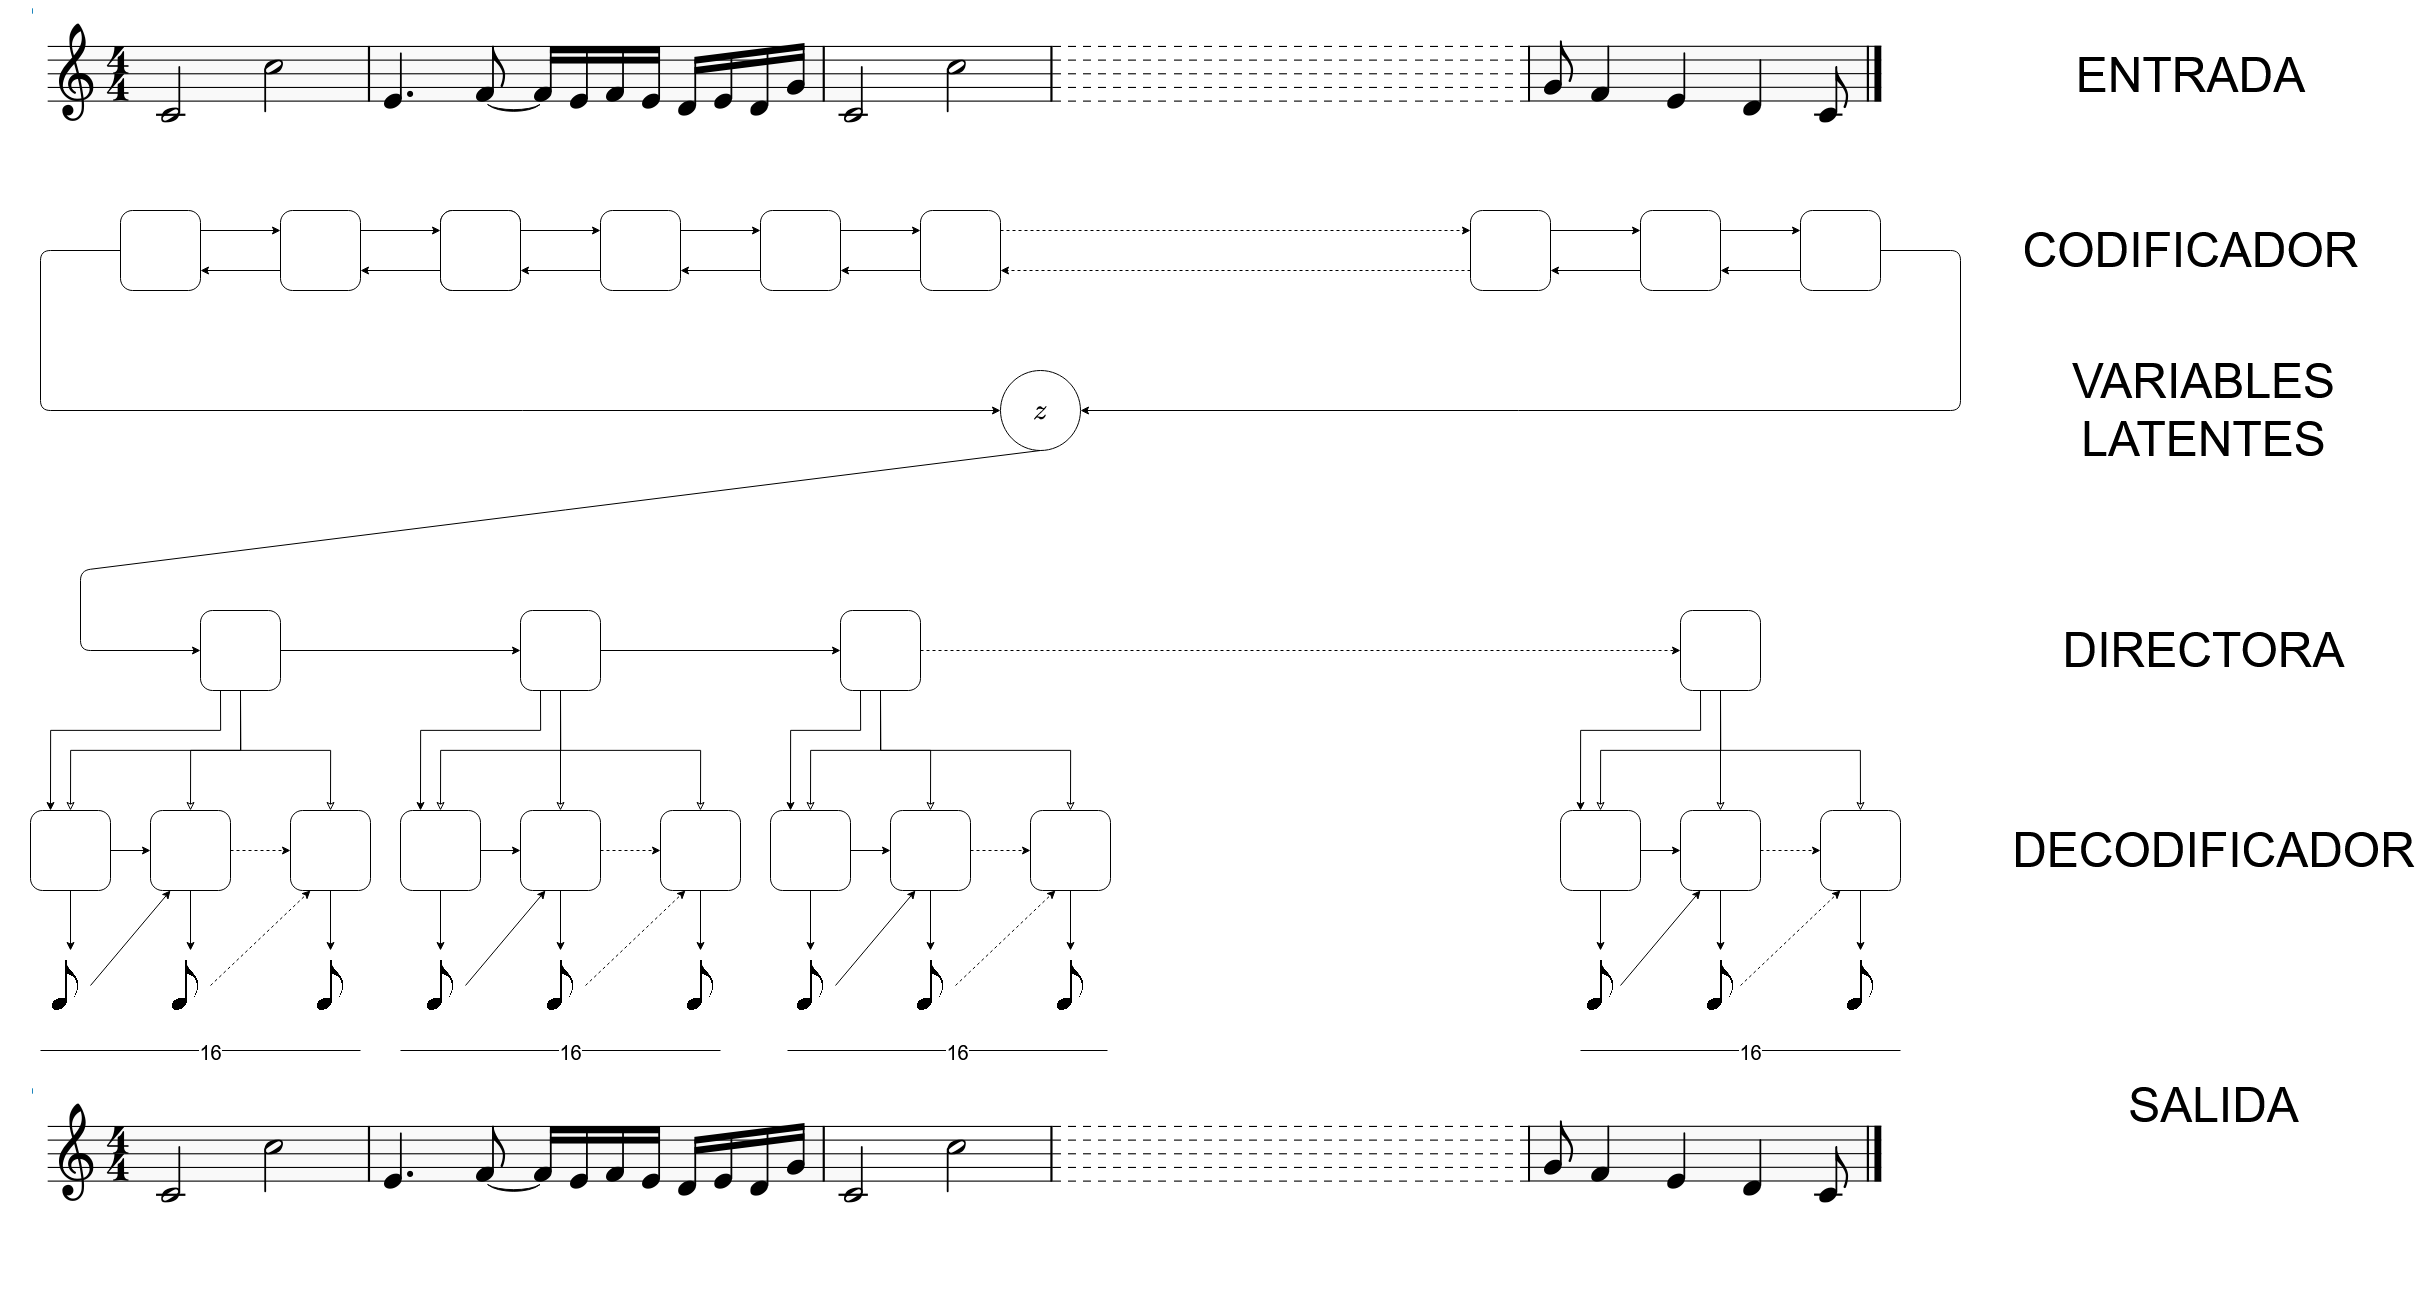
\includegraphics[width=1.1\textwidth]{musicvae}
  \caption{Estructura del modelo MusicVAE}
  \label{fig:musicvae}
\end{figure}


\section{Entrenamiento}

Para el entrenamiento se utilizaron archivos MIDI, que contienen instrucciones para que pueda ser reproducida cada nota de cada instrumento de una canción, así como información de medida (del tiempo). Fueron usados alrededor de 1,5 millones de estos archivos, de los cuales fueron extraídas melodías de 2 compases, melodías de 16 compases, percusiones de 2 y 16 compases y tríos (melodía, percusión y bajo) de 16 compases. Todos los archivos utilizados se encuentran en el compás de 4/4 y la unidad mínima de información considerada es la corchea (un dieciseisavo de compás). En total se obtuvieron $28$ millones de ejemplos diferentes para melodías de dos compases, $19,5$ millones para melodías de dieciséis compases, $3,8$ millones para percusiones de dos compases, $11,4$ millones para percusiones de dieciséis compases y $9,4$ millones para tríos.

Las melodías monofónicas se modelaron con un espacio de salida de dimensión $130$, con $128$ dimensiones representando el evento de ``pulsar una nota'' para cada uno de los $128$ tonos contemplados, un evento de ``dejar de tocar una nota'' y un evento de ``silencio''. Para la percusión se agruparon las sesenta y una clases de percusión del standard MIDI en 9 clases y se representaron todas las posibles combinaciones de golpes con 512 elementos categóricos. En ambos casos se consideran dieciséis eventos por compás, por lo que para los datos de dos compases se tiene $T = 32$ y para los de dieciséis compases se tiene $T = 256$. En todos los casos se utiliza $U = 16$, por lo que cada subsecuencia representa un compás completo. Todos los modelos se entrenan mediante el algoritmo Adam (\ref{adam}) con una tasa de aprendizaje entre $10^{-3}$ y $10^{-5}$, con ratio de decaimiento exponencial de $0,9999$ y tamaño de lotes de $512$. Los modelos de dos compases se entrenaron con $50000$ actualizaciones del gradiente y los de dieciséis compases con $100000$.

\section{Propiedades}

De la utilización del espacio latente para la representación de melodías se derivan ciertas propiedades que pueden ser explotadas en la utilización creativa de la herramienta que supone el modelo para la generación de música.

\subsection{Interpolación}\label{interpolate}

Dado un punto del espacio latente que se identifica con un dato real, los puntos cercanos en el espacio latente deberían corresponderse con datos reales parecidos. Esto implica que todos los puntos a través de una curva continua que conecta dos puntos en el espacio latente deberían ser identificables a una serie de ejemplos reales que produzcan una interpolación suave entre los ejemplos de los extremos. Para ello se requiere que el espacio latente no tenga regiones que no se identifiquen con ejemplos realistas. Estos requerimientos deberían cumplirse si ambos términos del ELBO son suficientemente bajos.

Una comprobación práctica de esta propiedad es realizar una interpolación entre puntos del espacio latente y comprobar si el resultado con sus correspondientes datos reales es adecuado. Dados $\textbf{z}_1$ y $\textbf{z}_2$ vectores latentes correspondientes a los datos $\textbf{x}_1$ y $\textbf{x}_2$, se puede realizar la interpolación lineal $$\textbf{c}_{\alpha} = \alpha \textbf{z}_1 + (1 - \alpha)\textbf{z}_2$$ para $\alpha \in [0,1]$. Se realizará la interpolación satisfactoriamente si para todo $\alpha$ el punto $p_\theta(\textbf{x} \vert \textbf{c}_\alpha)$ es un punto realista y la transición entre $p_\theta(\textbf{x} \vert \textbf{c}_0)$ y $p_\theta(\textbf{x} \vert \textbf{c}_1)$ se realiza de manera suave conforme se varía $\alpha$.

\subsection{Aritmética de vectores de atributos}

Otra propiedad deseada es la obtención de vectores de atributos, que son calculados como la media de los vectores latentes con una determinada característica. Si el modelo es capaz de generar dichos vectores, entonces podría cargarse un ejemplo con determinada característica y, sustrayendo el atributo correspondiente a dicha característica, eliminarla del dato real. Este mismo proceso debe poder realizarse para añadir una característica, sumando el vector de atributo.

Durante los experimentos realizados con el modelo se tomaron cinco características que pueden ser medidas en las melodías: pertenencia a las escala de Do diatónica, densidad de notas, intervalo medio y presencia de síncopas en la subdivisión de corcheas y semicorcheas. Las características fueron medidos en conjuntos de 370000 ejemplos y para cada una el conjunto fue ordenado en función de la cantidad de presencia del atributo. Se dividió entonces el conjunto en cuartiles y se calculó el vector del atributo restando a la media del vector lantente cuartil superior la media del vector latente del cuartil inferior. Después de generaron $256$ muestras aleatorias y se comprobó que sumar el vector obtenido producía un aumento en la característica correspondiente para la melodía. De igual manera la sustracción del vector producía una reducción en la medida de dicha característica.

\endinput
%------------------------------------------------------------------------------------
% FIN DEL CAPÍTULO.
%------------------------------------------------------------------------------------

% !TeX root = ../libro.tex
% !TeX encoding = utf8

\chapter{AutoLoops}

Como ejemplo de aplicación del contenido teórico del trabajo se ha desarrollado la herramienta AutoLoops, basada en el modelo MusicVAE de Magenta. Permite la manipulación sencilla del espacio latente de melodías de dos compases, permitiendo la codificación de una melodía ya existente y la exploración del espacio cercano para la generación de nuevos ejemplos relacionados.

La herramienta se inspira en las múltiples demostraciones ya  disponibles en la web que implementan los modelos desarrollados por Magenta, pero con pretensión de aplicación al proceso real de composición musical. Desde su concepción inicial se establece no solo como un ejemplo de las capacidades del modelo, sino también como una herramienta que pueda ser utilizada directamente por artistas en el contexto real de la composición y producción musical.

En cuanto a su utilización, la herramienta se basa en el método de trabajo que muchas veces se utiliza para el diseño sonoro en los sintetizadores. Estos permiten la generación y modificación de ondas sonoras para la creación de timbres. Muchas veces es difícil entender la repercusión exacta que tendrá en el sonido producido la modificación de alguna de estas características, o la interacción entre varias de estas modificaciones. Es por ello que muchas veces la construcción de un sonido se realiza explorando el espacio que las características ofrecen mediante el método de prueba y error.

Se trata por tanto de traducir este método al trabajo con melodías. Mediante el modelo MusicVAE (\autoref{modelo}) se obtienen las características de una melodía, aunque su significado es oculto. El artista puede cargar su propia melodía y generar nuevas a partir de la misma modificando las características que se le proporcionan. Podrá generar una secuencia de melodías de dos compases o una sola melodía que podrá exportar como archivo MIDI, que puede usarse en la producción de una canción.

\begin{figure}[htpb]
  \centering
  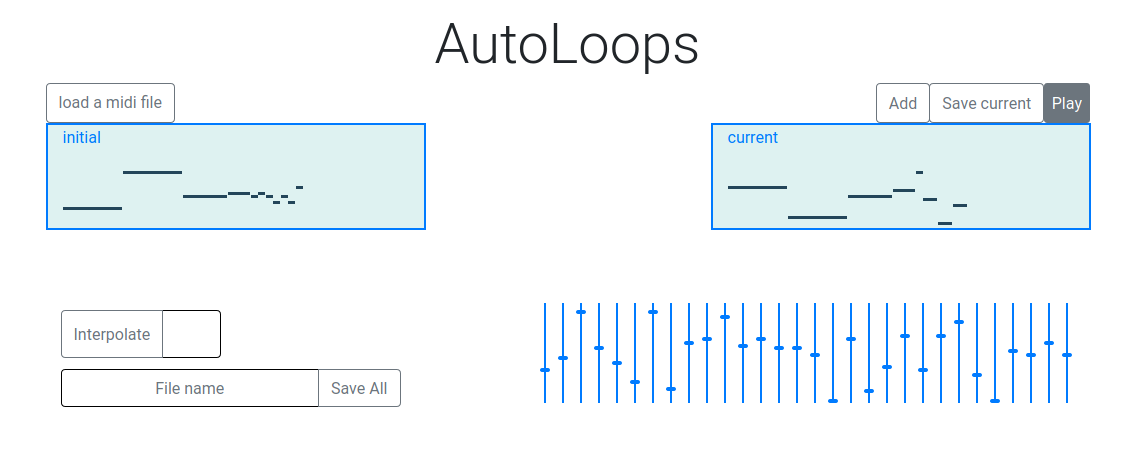
\includegraphics[width=1.1\textwidth]{autoloops}
  \caption{Interfaz de AutoLoops}
  \label{fig:autoloops}
\end{figure}

\section{Marco de trabajo}

La herramienta se ha desarollado en forma de aplicación web para la que se ha utilizado HTML y CSS para el diseño de la interfaz y JavaScript para el funcionamiento interno.

\subsection{HTML}

Para la maquetación de la interfaz se ha utilizado HTML, lenguaje de marcado estándar a cargo del \textit{World Wide Web Consortium} (W3C). Sobre este se ha utilizado la biblioteca Bootstrap para el diseño con sistema de rejilla. Puede incluirse dicha biblioteca mediante la siguiente línea en la cabecera.

\begin{lstlisting}
<link rel="stylesheet" href="https://stackpath.bootstrapcdn.com/bootstrap/4.5.2/css/bootstrap.min.css">
\end{lstlisting}

Además también se ha utilizado una hoja de estilos CSS.

\subsection{CSS}

Mientras que HTML tiene el contenido de la interfaz, la hoja CSS contiene el diseño de los elementos de la misma. Para su inclusión se debe añadir la siguiente línea en la cabecera.

\begin{lstlisting}
<link rel="stylesheet" href="assets/css/index.css">
\end{lstlisting}

\subsection{JavaScript}

Para la programación del funcionamiento de la aplicación se utiliza JavaScript, un lenguaje de programación interpretado utilizado principalmente en páginas web y aplicaciones de servidor. Para exportar los archivos MIDI necesarios se ha utilizado la biblioteca FileSaver, que se incluye mediante la siguiente línea en la cabecera del archivo HTML.

\begin{lstlisting}
<script src="https://cdnjs.cloudflare.com/ajax/libs/FileSaver.js/1.3.8/FileSaver.min.js" defer></script>
\end{lstlisting}

Para la visualización de datos se utiliza la biblioteca D3, que se incluye mediante la siguiente línea en la cabecera del archivo HTML.

\begin{lstlisting}
<script src="https://cdnjs.cloudflare.com/ajax/libs/d3/5.15.0/d3.js"></script>
\end{lstlisting}

Por último, y aquella con uso más extensivo por ser la que aporta el núcleo de la funcionalidad del programa, se ha utilizado la biblioteca Magenta.js.

\subsection{Biblioteca Magenta.js}

La biblioteca Magenta.js provee al desarrollador de una API de alto nivel para la aplicación de modelos de aprendizaje automático, especialmente aprendizaje profundo, para el modelado y manipulación de datos relacionados con el arte como imágenes y música. Está desarrollada sobre TensorFlow, una biblioteca para la creación de modelos de aprendizaje automático~\cite{magentajs}.

El paquete \textit{magenta/music} contiene una API para JavaScript para la interacción con modelos para la generación de música. Puede incluirse añadiendo la siguiente línea en la cabecera del archivo HTML.

\begin{lstlisting}
<script src="https://cdn.jsdelivr.net/npm/@magenta/music@1.12.1/dist/magentamusic.min.js"></script>
\end{lstlisting}

El paquete contiene dos funcionalidades principales: procesamiento de datos y API para modelos, incluídos modelos pre-entrenados.

\subsubsection{Procesamiento de datos}

Se establece la clase $\textit{NoteSequence}$ como representación de partituras musicales. Esta representación almacena aspectos fundamentales de una secuencia de notas como son tiempos, tonos e instrumentos, pero también metadatos como etiquetas de secciones o información sobre acordes. El paquete también contiene una re-implementación de la librería $\textit{NoteSequence}$ de Magenta Python, que incluye funcionalidades para convertir MIDI en $\textit{NoteSequence}$ y viceversa, así como para la síntesis y reproducción de sonido. También existe la posibilidad de convertir las $\textit{NoteSequence}$ en tensores de la biblioteca TensorFlow, que son utilizados como entrada y salida de los modelos.

\subsubsection{Interfaces de modelos}

La biblioteca también incluye interfaces para los múltiples modelos de Magenta. Entre los modelos dedicados a la música se encuentran interfaces para MusicRNN~\cite{performance-rnn-2017}, MidiMe~\cite{midime}, Piano Genie~\cite{pianogenie}, GANSynth~\cite{engel2019gansynth}, y el modelo que se utiliza en este proyecto, MusicVAE.

Con respecto a este último modelo se implementan métodos que incluyen \textit{encode} y \textit{decode} para codificar \textit{NoteSequence} en vectores latentes y al revés. Además se añaden los métodos \textit{interpolate} para facilitar la operación de interpolación entre melodías (\autoref{interpolate}) y \textit{sample} para generar muestras de melodías.

Para evitar que el desarrollador tenga que llevar a cabo la costosa operación del entrenamiento del modelo se facilitan también archivos con los pesos del modelo. Estos se facilitan en forma de archivos de configuración JSON. En este caso utilizamos el modelo de MusicVAE para melodías de dos compases, por lo que cargamos el modelo mediante

\begin{lstlisting}
const model = new mm.MusicVAE('https://storage.googleapis.com/magentadata/js/checkpoints/music_vae/mel_2bar_small');
\end{lstlisting}

\section{Uso de la aplicación}

Para abrir la aplicación el usuario solo debe descargar los archivos y abrir $\textit{index.html}$ con un navegador. Hecho esto se visualizará la interfaz de la  \autoref{fig:autoloops}.

Para comenzar a utilizar la herramienta el usuario deberá cargar una melodía en formato MIDI monofónica de dos compases. Esta acción puede llevarse a cabo mediante el botón \textit{load a midi file}, que permitirá elegir el archivo sobre el que se quiere trabajar. Una vez la melodía ha sido introducida se mostrará en los cuadros \textit{initial} y \textit{current}.

\begin{figure}[htpb]
  \centering
  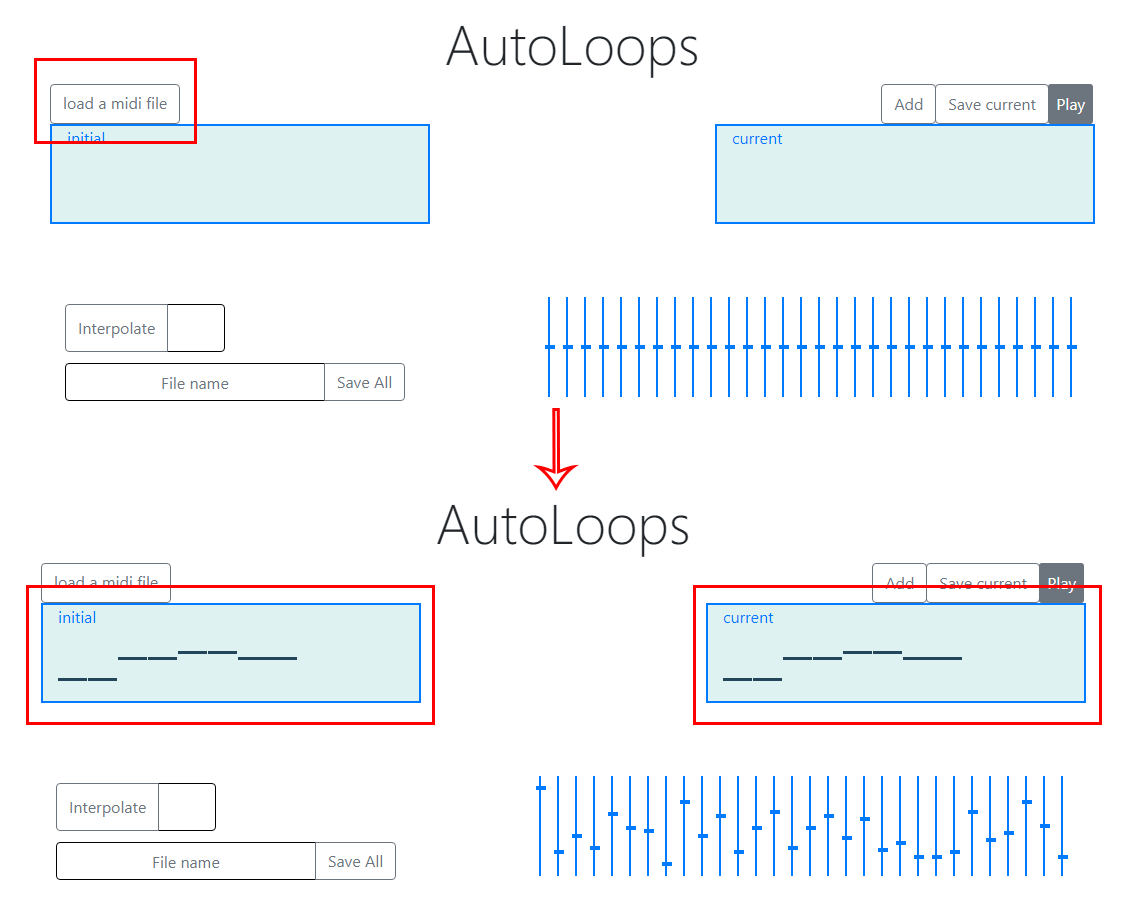
\includegraphics[width=1.1\textwidth]{loadmelody}
  \caption{Cargar una melodía a AutoLooops}
  \label{fig:loadmelody}
\end{figure}


Una vez la melodía está cargada puede comenzarse a generar nuevas melodías a partir de la misma. Los controles deslizantes reflejarán las características en el espacio latente de la melodía que se ha cargado. El usuario puede modificarlas y con ello se generarán nuevas melodías. El cambio podrá apreciarse visualmente en el cuadro \textit{current}, que mostrará la melodía correspondiente a la codificación actual marcada por los controles deslizantes. La melodía actual podrá también escucharse mediante el botón \textit{play}.

\begin{figure}[htpb]
  \centering
  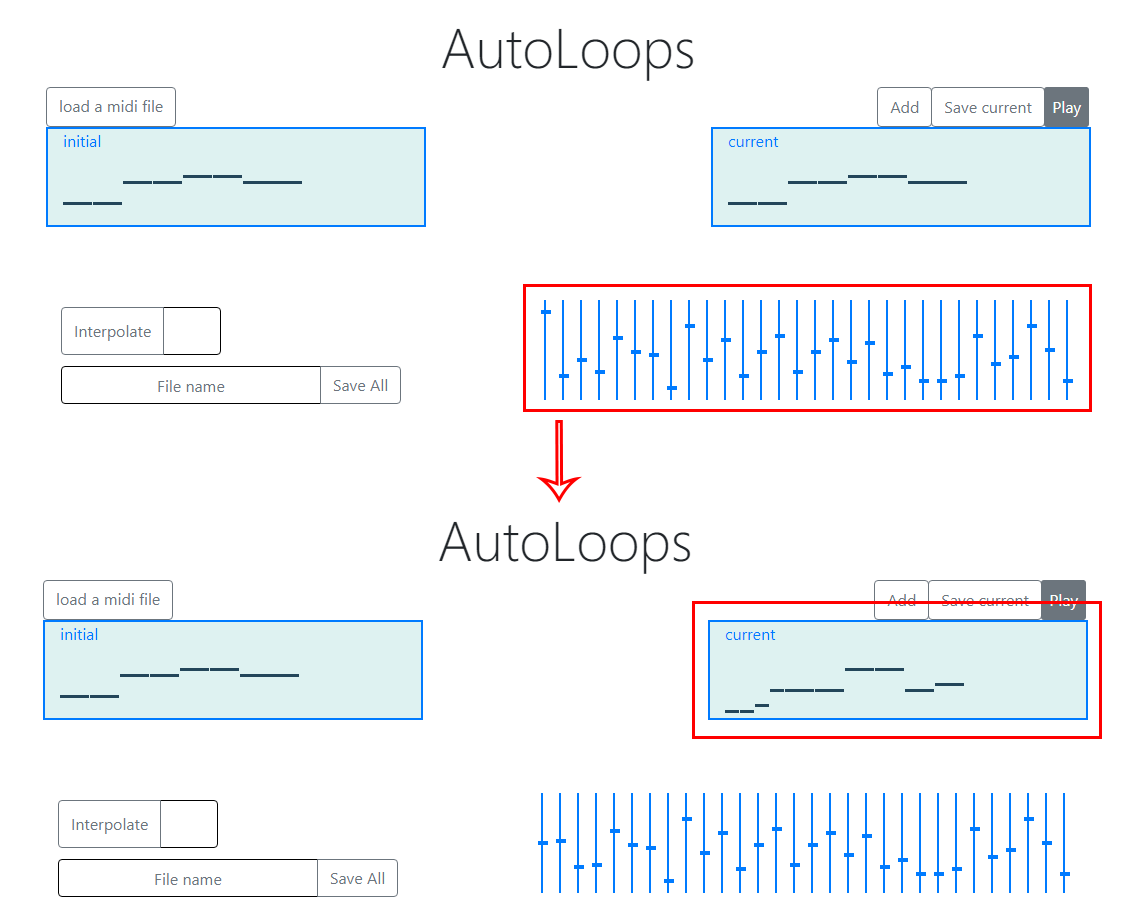
\includegraphics[width=1.1\textwidth]{changemelody}
  \caption{Crear una nueva melodía a AutoLooops}
  \label{fig:changemelody}
\end{figure}

Cada vez que el usuario lo considere oportuno puede utilizar el botón \textit{add} para guardar la melodía actual. Estas melodías guardadas podrán ser después exportadas como una secuencia completa mediante el botón \textit{save all}, que también cuenta con un campo para recoger el nombre para el archivo MIDI en el que se exportarán las melodías.

\begin{figure}[htpb]
  \centering
  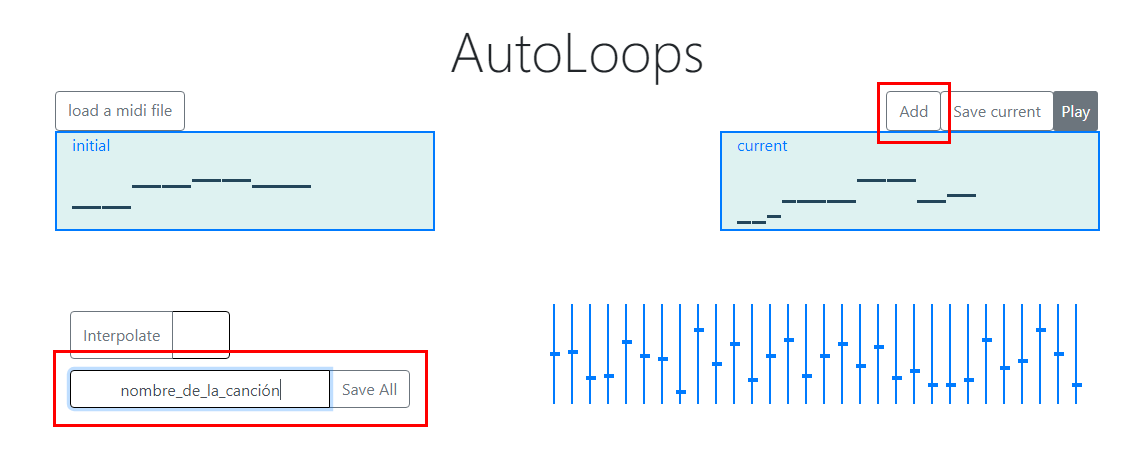
\includegraphics[width=1.1\textwidth]{savemelody}
  \caption{Guardar y exportar una secuencia de melodías en AutoLoops}
  \label{fig:savemelody}
\end{figure}

También puede exportarse únicamente la melodía actual mediante el botón \textit{save current}.

\begin{figure}[htpb]
  \centering
  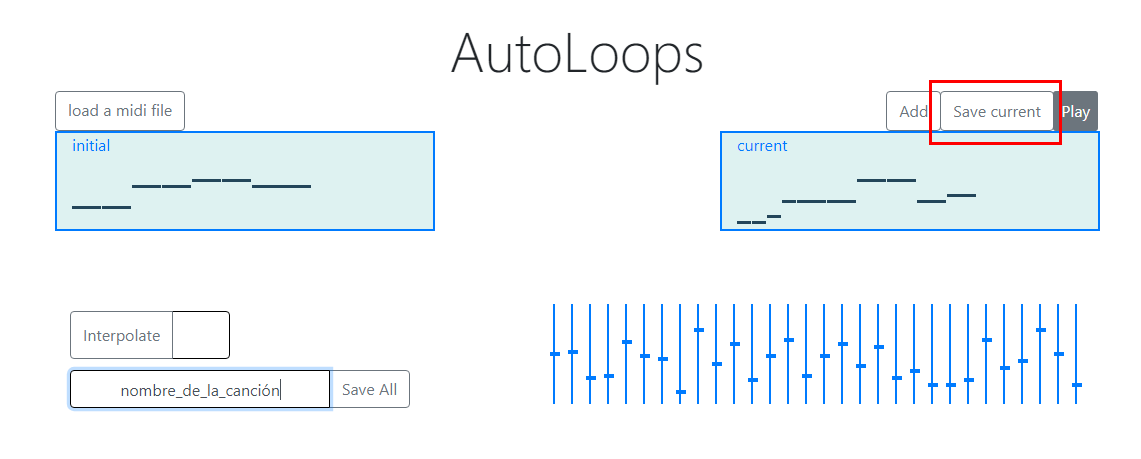
\includegraphics[width=1.1\textwidth]{savecurrentmelody}
  \caption{Exportar la melodía actual en AutoLoops}
  \label{fig:savecurrentmelody}
\end{figure}

Por último se ofrece también la posibilidad de interpolar entre la melodía actual y la melodía inicial. Para ello se hará uso del botón \textit{interpolate}, junto al que se incluye un campo para recoger el número de pasos que se quieren realizar. El usuario puede introducir un número y se guardará una interpolación entre la melodía de \textit{current} y la de \textit{initial} con ese número de melodías, siendo la primera de la secuencia la melodía actual y la última la melodía inicial. Hecho esto la melodía inicial pasará a ser la actual y puede proseguirse con la utilización del programa.

\begin{figure}[htpb]
  \centering
  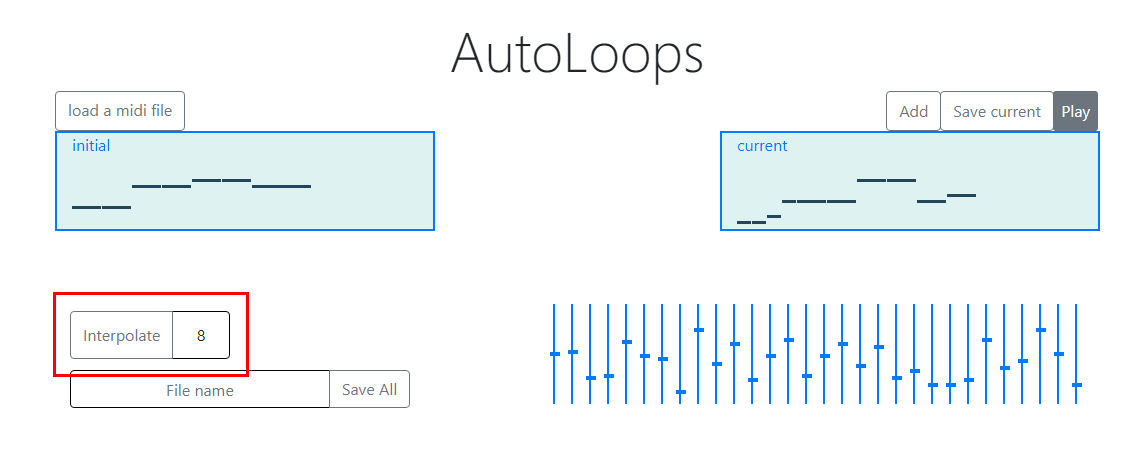
\includegraphics[width=1.1\textwidth]{interpolatemelody}
  \caption{Intepolación entre la melodía actual y la inicial en 8 pasos}
  \label{fig:savemelody}
\end{figure}

\section{Funcionamiento interno}

Comprendida la estructura general del programa puede detallarse su funcionamiento. Cuando el usuario carga una melodía MIDI se utiliza el método \textit{blobToNoteSequence} facilitado por la biblioteca \textit{magenta music} para convertir la secuencia cargada en un objeto del tipo \textit{NoteSequence}, que es la representación de melodías con las que se trata. Se utiliza entonces el modelo de MusicVAE para obtener la codificación de la melodía mediante el método \textit{encode}. Con la codificación obtenida se actualizan los controles deslizantes, haciendo que su posición corresponda al valor de la variable latente correspondiente. Hecho esto se decodifica la melodía mediante el método \textit{decode} y se toma dicha decodificación como melodía inicial y melodía actual. Por último se visualizan las melodías mediante el método \textit{PianoRollSVGVisualizer}, también de la biblioteca \textit{magenta music}.

Una vez establecidas las melodías inicial y actuales pueden moverse los controles deslizantes. Cualquier movimiento se captura y se maneja, creando un tensor con los valores modificados y decodificando dicho tensor para obtener la melodía actual.

Cada vez que se pulsa \textit{add} la melodía actual es añadida a las melodías ya guardadas. Se cuenta con una instancia de \textit{NoteSequence} para almacenar estas melodías. Cada vez que se concatena la que contiene las guardadas con la actual. Esta acción se realiza mediante el método \textit{concatenate} de \textit{magenta music}.

Cuando el usuario pulsa el botón \textit{save all} las melodías guardadas son exportadas a un archivo MIDI del nombre que el usuario elija. Para ello primero se transforma la melodía de \textit{NoteSequence} a MIDI mediante el método \textit{sequenceProtoToMidi} de \textit{magenta music}. Hecho esto el archivo se guarda mediante la función \textit{saveAs} de la biblioteca \textit{FileSaver}. De la misma manera cuando se pulsa \textit{save current} se transforma solo la melodía actual y se exporta.

Para realizar la interpolación se utiliza el método \textit{interpolate} correspondiente al modelo MusicVAE. Se toma como primera melodía de la interpolación la melodía actual y como última la melodía inicial, y se generan una secuencia de tantos pasos como los indicados por el usuario. Hecho esto cada elemento de la secuencia se añade a las secuencias guardadas.

\endinput
%------------------------------------------------------------------------------------
% FIN DEL CAPÍTULO.
%------------------------------------------------------------------------------------

% !TeX root = ../libro.tex
% !TeX encoding = utf8

\chapter{Conclusiones y trabajo futuro}

En este trabajo se ha estudiado la aplicación de las técnicas de aprendizaje profundo a la generación de música, desde los fundamentos teóricos hasta la aplicación práctica mediante un programa para su uso en el proceso de composición real.

Como punto de partida se ha estudiado el teorema de aproximación universal, que establece el poder de representación que tienen las redes neuronales. Se han repasado los resultados previos necesarios para su demostración y realizado la misma, para terminar con otros resultados que generalizan o complementan este.

A continuación se han tratado cuestiones básicas sobre aprendizaje profundo, incluyendo su contextualización dentro del aprendizaje automático, la definición del modelo más simple, la red profunda prealimentada, y los algoritmos necesarios para la optimización de los mismos.

Más adelante se han tratado las técnicas que ofrece el aprendizaje profundo para el tratamiento de secuencias, esencial para el trabajo con música por la naturaleza secuencial de la misma. Se ha introducido el modelo básico para este fin, la red neuronal recurrente, y los modelos más actuales en este ámbito.

Tras esto se han repasado técnicas para el aprendizaje de características, que permiten el tratamiento simplificado de datos de naturaleza compleja como lo son aquellos derivados de la música. Se ha hecho especial hincapié en los modelos de aprendizaje automático y de entre ellos en el \textit{autoencoder} variacional, que cumple también la función de modelo generativo. El estudio de este modelo se ha realizado desde la perspectiva teórica de la inferencia estadística, habiéndose completado con la obtención de la expresión explícita de su ELBO.

Estudiados los fundamentos teóricos se ha introducido un modelo dirigido a la generación de música, el MusicVAE. Se han discutido su estructura y características básicas, así como el proceso de entrenamiento y las funcionalidades que ofrece.

Por último se ha desarrollado una implementación práctica del modelo en una herramienta llamada AutoLoops. La herramienta, basada en la biblioteca de Magenta que funciona como API para el modelo, se ha planteado como una herramienta para la exploración del espacio latente cuyo objetivo es la generación de melodías. Esta herramienta tiene pretensión de ser utilizada en el contexto real de la composición musical, y de hecho ya está siendo aplicada en la creación de obras musicales. Algunas de estas obras pueden encontrarse en \href{https://soundcloud.com/user-860813847/sets/autoloops}{este enlace}.

Con esto se considera que los objetivos iniciales marcados para el trabajo han sido cumplidos. Sin embargo, la realización del mismo deja abiertas varias vías de trabajo futuras:

\begin{itemize}
\item Inclusión en la herramienta AutoLoops de capacidad para ver y manipular las melodías guardadas.
\item Mejora del reproductor de sonido de la herramienta, permitiendo cambiar el tempo de reproducción de las melodías y el timbre con el que se reproducen.
\item Adaptación de la herramienta para su utilización en interpretaciones musicales en directo, permitiendo fijar un tempo y reproducir en bucle la melodía actual a ese tempo, pudiendo además modificarla a la vez.
\item Adaptación de la herramienta para que pueda ser utilizada como controlador MIDI, para poder así manejar dispositivos  externos directamente desde la herramienta.
\item Implementación en la herramienta del resto de variantes del modelo MusicVAE, permitiendo así la generación de secuencias de percusión, tríos y melodías de 12 compases.
\item Implementación de herramientas similares a AutoLoops basadas en otros modelos actuales para facilitar el acceso de artistas a modelos de aprendizaje profundo que permiten nuevas formas de generar y manipular música.
\end{itemize}

\endinput
%------------------------------------------------------------------------------------
% FIN DEL CAPÍTULO.
%------------------------------------------------------------------------------------


% --------------------------------------------------------------------
% APPENDIX: Opcional
% --------------------------------------------------------------------

\appendix % Reinicia la numeración de los capítulos y usa letras para numerarlos
\pdfbookmark[-1]{Apéndices}{appendix} % Alternativamente podemos agrupar los apéndices con un nuevo \part{Apéndices}

%% !TeX root = ../libro.tex
% !TeX encoding = utf8

\chapter{Primer apéndice}\label{ap:apendice1}

Los apéndices son opcionales.

Archivo: \texttt{apendices/apendice01.tex}

\endinput
%------------------------------------------------------------------------------------
% FIN DEL APÉNDICE. 
%------------------------------------------------------------------------------------

% Añadir tantos apéndices como sea necesario

% --------------------------------------------------------------------
% GLOSARIO: Opcional
% --------------------------------------------------------------------

%% !TeX root = ../libro.tex
% !TeX encoding = utf8

\chapter*{Glosario}
\addcontentsline{toc}{chapter}{Glosario} % Añade el glosario a la tabla de contenidos

La inclusión de un glosario es opcional.

Archivo: \texttt{glosario.tex}

\begin{description} 
  \item[$\mathbb{R}$] Conjunto de números reales.

  \item[$\mathbb{C}$] Conjunto de números complejos.

  \item[$\mathbb{Z}$] Conjunto de números enteros.
\end{description}
\endinput


% -------------------------------------------------------------------
% BACKMATTER
% -------------------------------------------------------------------

\backmatter % Desactiva la numeración de los capítulos
\pdfbookmark[-1]{Referencias e Índices}{BM-Referencias}

% BIBLIOGRAFÍA
%-------------------------------------------------------------------

\setbibpreamble{Las referencias se listan por orden alfabético. Aquellas referencias con más de un autor están ordenadas de acuerdo con el primer autor.\par\bigskip}
\bibliographystyle{alpha}
\begin{small} % Normalmente la bibliografía se imprime en un tamaño de letra más pequeño.
\bibliography{library.bib}
\end{small}


% ÍNDICE TERMINOLÓGICO  (Opcional)
%-------------------------------------------------------------------

\cleardoublepage
\setindexpreamble{Todos los números impresos en \textbf{negrita} hacen referencia a la página donde se encuentra la definición del término. Los números de página impresos normalmente hacen referencia a las páginas donde dicho término es usado.\par\bigskip}
\begin{footnotesize} % Normalmente el índice se imprime en un tamaño de letra más pequeño.
\printindex
\end{footnotesize}

\end{document}
